\documentclass[twoside]{book}

% Packages required by doxygen
\usepackage{fixltx2e}
\usepackage{calc}
\usepackage{doxygen}
\usepackage[export]{adjustbox} % also loads graphicx
\usepackage{graphicx}
\usepackage[utf8]{inputenc}
\usepackage{makeidx}
\usepackage{multicol}
\usepackage{multirow}
\PassOptionsToPackage{warn}{textcomp}
\usepackage{textcomp}
\usepackage[nointegrals]{wasysym}
\usepackage[table]{xcolor}

% NLS support packages
\usepackage{hfont}

% Font selection
\usepackage[T1]{fontenc}
\usepackage[scaled=.90]{helvet}
\usepackage{courier}
\usepackage{amssymb}
\usepackage{sectsty}
\renewcommand{\familydefault}{\sfdefault}
\allsectionsfont{%
  \fontseries{bc}\selectfont%
  \color{darkgray}%
}
\renewcommand{\DoxyLabelFont}{%
  \fontseries{bc}\selectfont%
  \color{darkgray}%
}
\newcommand{\+}{\discretionary{\mbox{\scriptsize$\hookleftarrow$}}{}{}}

% Page & text layout
\usepackage{geometry}
\geometry{%
  a4paper,%
  top=2.5cm,%
  bottom=2.5cm,%
  left=2.5cm,%
  right=2.5cm%
}
\tolerance=750
\hfuzz=15pt
\hbadness=750
\setlength{\emergencystretch}{15pt}
\setlength{\parindent}{0cm}
\setlength{\parskip}{3ex plus 2ex minus 2ex}
\makeatletter
\renewcommand{\paragraph}{%
  \@startsection{paragraph}{4}{0ex}{-1.0ex}{1.0ex}{%
    \normalfont\normalsize\bfseries\SS@parafont%
  }%
}
\renewcommand{\subparagraph}{%
  \@startsection{subparagraph}{5}{0ex}{-1.0ex}{1.0ex}{%
    \normalfont\normalsize\bfseries\SS@subparafont%
  }%
}
\makeatother

% Headers & footers
\usepackage{fancyhdr}
\pagestyle{fancyplain}
\fancyhead[LE]{\fancyplain{}{\bfseries\thepage}}
\fancyhead[CE]{\fancyplain{}{}}
\fancyhead[RE]{\fancyplain{}{\bfseries\leftmark}}
\fancyhead[LO]{\fancyplain{}{\bfseries\rightmark}}
\fancyhead[CO]{\fancyplain{}{}}
\fancyhead[RO]{\fancyplain{}{\bfseries\thepage}}
\fancyfoot[LE]{\fancyplain{}{}}
\fancyfoot[CE]{\fancyplain{}{}}
\fancyfoot[RE]{\fancyplain{}{\bfseries\scriptsize 다음에 의해 생성됨 \+:  Doxygen }}
\fancyfoot[LO]{\fancyplain{}{\bfseries\scriptsize 다음에 의해 생성됨 \+:  Doxygen }}
\fancyfoot[CO]{\fancyplain{}{}}
\fancyfoot[RO]{\fancyplain{}{}}
\renewcommand{\footrulewidth}{0.4pt}
\renewcommand{\chaptermark}[1]{%
  \markboth{#1}{}%
}
\renewcommand{\sectionmark}[1]{%
  \markright{\thesection\ #1}%
}

% Indices & bibliography
\usepackage{natbib}
\usepackage[titles]{tocloft}
\setcounter{tocdepth}{3}
\setcounter{secnumdepth}{5}
\makeindex

% Hyperlinks (required, but should be loaded last)
\usepackage{ifpdf}
\ifpdf
  \usepackage[pdftex,pagebackref=true]{hyperref}
\else
  \usepackage[ps2pdf,pagebackref=true]{hyperref}
\fi
\hypersetup{%
  colorlinks=true,%
  linkcolor=blue,%
  citecolor=blue,%
  unicode%
}

% Custom commands
\newcommand{\clearemptydoublepage}{%
  \newpage{\pagestyle{empty}\cleardoublepage}%
}

\usepackage{caption}
\captionsetup{labelsep=space,justification=centering,font={bf},singlelinecheck=off,skip=4pt,position=top}

%===== C O N T E N T S =====

\begin{document}

% Titlepage & ToC
\hypersetup{pageanchor=false,
             bookmarksnumbered=true,
             pdfencoding=unicode
            }
\pagenumbering{alph}
\begin{titlepage}
\vspace*{7cm}
\begin{center}%
{\Large Comet\+Engine \\[1ex]\large 0.\+0.\+1 }\\
\vspace*{1cm}
{\large 다음에 의해 생성됨 \+:  Doxygen 1.8.13}\\
\end{center}
\end{titlepage}
\clearemptydoublepage
\pagenumbering{roman}
\tableofcontents
\clearemptydoublepage
\pagenumbering{arabic}
\hypersetup{pageanchor=true}

%--- Begin generated contents ---
\chapter{Comet\+Engine}
\label{md__r_e_a_d_m_e}
\Hypertarget{md__r_e_a_d_m_e}
\subsection*{Introduction}

\+\_\+( 영알못이라 밑에 영어로 대충 써놓은건 아무말 대잔치. 젠장. )\+\_\+

\paragraph*{현제 개발 초기 (기획)단계입니다.}

\paragraph*{아직은 보여드릴게 많지 않지만 꾸준히 방문해 주시면 감사하겠습니다. ( \+\_\+ \+\_\+ )}

{\bfseries Comet Engine} 은 윈도우 게임 개발자들을 위해 개발되고 있는 오픈소스 게임엔진입니다.

Win32와 U\+W\+P를 같은 코드로 동작 하게끔 개발 할 예정입니다.

Comet\+Engine은 Client -\/ Server간의 개발을 쉽게끔 할 수 있도록 도와줄 것 입니다.

\subsection*{Documentation.}

\href{https://devsdk.github.io/CometEngine/html/index.html}{\tt Link }

\subsection*{Engine Architecture}

U\+W\+P와 Win32를 동시에 지원.

\hyperlink{namespace_comet_engine}{Comet\+Engine} Builder를 개발해 U\+WP, Win32로 빌드 할 수 있게끔 개발할 예정 -\/$>$ 연구가 필요.

Comet\+Engine의 모듈들\+: \begin{DoxyVerb}CometEngineCommon
    CometEngine.dll
    CometEngineCollision.dll
    CometEngineFiles.dll
    CometEngineGeometry.dll
    CometEngineNetwork.dll
    CometEngineLibs.dll
CometEngineClient
    CometEngineDXRenderer.dll
    CometEngineWin32.dll
CometEngineServer
    CometEngineDB.dll
\end{DoxyVerb}


※\+\_\+\+\_\+\+Comet\+Engine Editor\+\_\+\+\_\+ 는 추후에 추가 될 예정입니다.

{\bfseries Common} 은 클라이언트와 서버 사이에 공통된 라이브러리, 도구, 엔진등등을 포함하고 있는 모듈 집합입니다.

{\bfseries Client} 는 Windows 클라이언트를 위한 도구들을 포함하고 있는 모듈입니다. \mbox{[}Win32 Desk\+Top\mbox{]}

{\bfseries Server} Multi-\/\+Core Processing, G\+P\+G\+P\+U를 활용해 효율적으로 서버를 처리하고, 데이터베이스관련 도구를 제공

게임 개발자가 사용할 스크립트 언어는 C\+::입니다.

게임엔진 내부는 C++로 구성되어 있고, D\+L\+L로 제공됩니다.

\subsection*{Design of Librarys}

난수를 생성 라이브러리를 자체 제공한다. ex) 메르센 트위스터

파일을 zip형태로 압축하거나, 리소스를 직접 컴파일함\mbox{[}암호화 지원\mbox{]}

• 잘 알려진 파일 형식 ex) P\+NG, J\+P\+EG, B\+MP 등등은 에디터에 불러와 파싱

• 자체적인 에니메이션 메커니즘이 필요 (리깅, 스켈레톤 등) \begin{DoxyVerb}-만약 필요할경우, Blender 같은 Util에서 만드는 데이터를 파싱할 필요 있음.
\end{DoxyVerb}


• 네트워크의 경우 Serializer를 제공, Bit 단위 전송을 최대한 지원. \begin{DoxyVerb} -C# 자체 통신은 사용하지 않고 C++ WinSock을 사용할 것, 다만 Wrapping에 주의
\end{DoxyVerb}


• 게임게발자가 로우레벨 시스템을 고려하지 않도록 설계하면서도 언제든지 로우레벨에 접근이 가능하도록 설계

• In-\/\+Game Profiler을 개발해 C\+PU,G\+PU, Memeory, Allocation등등을 수집 및 출력

• 필요할 경우 구조를 State Machine + Pipe Line로 모듈을 구성 \begin{DoxyVerb}    - ex) Animation Pipeline, Resource Processing PipeLine, etc..
\end{DoxyVerb}


\subsection*{Optimazation\+:}

S\+SE 명령어 사용 ( 다중 명령어 병렬처리 기법 ) -\/ 하드웨어 가속 가능 \begin{DoxyVerb}• __m128
• 전용 레지스터 ( 16바이트 범위 보장 )
• __declspec(align(16)) type []
• MSDN 찾아볼것
\end{DoxyVerb}


메모리 Allocator구현 및 제공 \begin{DoxyVerb}• 게임엔진 내에서 사용할 자료구조에 적용하면 효율적일 것으로 예상됨. ex) 렌더링 커멘드
\end{DoxyVerb}


파티클 시스템을 연구할 필요가 있음. Particle의 경우 자체를 State Machine으로 만들어 G\+PU 에서 처리하는 쪽으로 구상중

가능하다면 Collision Detection을 G\+P\+G\+P\+U로 구성

Open\+MP 적극 활용 ( Loop 루틴, 산술연산 등)

\subsection*{License\+:}

B\+SD License.

~\newline
 ~\newline
 



\section*{Comet Engine}

\subsection*{Introduction}

{\bfseries \hyperlink{namespace_comet_engine}{Comet\+Engine}} is Open Source Game Engine for Windows Game Developers

Support Build Win32 and U\+WP using same code.

This project is in the early stages of development.

So, I can\textquotesingle{}t show Engine Document not yet

\subsection*{Engine Architecture}

Support Build Win32 and U\+WP at the same code\+:

Probably Develop \textquotesingle{}\hyperlink{namespace_comet_engine}{Comet\+Engine} Builder\textquotesingle{} that module can U\+WP Win32 Build support

The Comet Engine Modules\+: \begin{DoxyVerb}CometEngineCommon
  CometEngine.dll
  CometEngineCollision.dll
  CometEngineFiles.dll
  CometEngineGeometry.dll
  CometEngineNetwork.dll
  CometEngineLibs.dll
CometEngineClient
  CometEngineDXRenderer.dll
  CometEngineWin32.dll
CometEngineServer
  CometEngineDB.dll
\end{DoxyVerb}


※\+\_\+\+\_\+\+Comet\+Engine Editor\+\_\+\+\_\+ will add later.

The {\bfseries Common} is Common Modules Server and Client side

The {\bfseries Client} is Client Modules for Windows Client \mbox{[} Win32 Desk\+Top, U\+WP\mbox{]}

The {\bfseries Server} is Server Modules for Server side. That can support G\+P\+G\+UP, DB, Multi-\/\+Core

The Script Language is C\# for Game Developer.

Game Engine Layer implement C++ Language and Provide D\+LL

\subsection*{Design Of Librarys}

•\+Provide Random Number Library. ex) Mersenne Twister, or external library

•\+Compress Resources like zip file or Compile Resource. \mbox{[}Support Encryption\mbox{]}

• Load to Editor and parsing data Well-\/\+Known File Format ex) P\+NG, J\+P\+EG, B\+MP and E\+TC

• Probably Need Own Animation Method ( Rigging, Skeleton ) \begin{DoxyVerb}- Probably Need Parsing Data from well-known utils ex) Blender.
\end{DoxyVerb}


• Network Module support Serializer, and make sure send a bit data. \begin{DoxyVerb} - Do Not Use ".Net"and "C# Socket." Using C++ WinSock. and make sure Wrapping.
\end{DoxyVerb}
 • Make sure the Game Developer focus on High-\/\+Level. But The \hyperlink{namespace_comet_engine}{Comet\+Engine} provide Low-\/\+Level System

• Develop In-\/\+Game Profiler. For C\+PU,G\+PU, Memeory and Allocation Information Collect and Visualize

• If I Need, module strcuture change to State Machine + Pipe Line \begin{DoxyVerb}- ex) Animation Pipeline, Resource Processing PipeLine, etc..
\end{DoxyVerb}


\subsection*{Optimazation}

Using S\+SE Operation and Hard-\/ware Acceleration \begin{DoxyVerb}• __m128

• Own Register

• __declspec(align(16)) type []

•  Read More MSDN 
\end{DoxyVerb}


Memory Allocator Implementation and provide \begin{DoxyVerb}• Using Engine Core Data-Structure ex) Render Command
\end{DoxyVerb}


I Need More Research The Particle System. My Opinion is Particle make to State Machine and processing G\+PU Level.

If I can, G\+P\+G\+PU Collision Detection

Using Open\+MP

\subsection*{License\+:}

B\+SD License.

~\newline
 ~\newline
 
\chapter{네임스페이스 색인}
\section{네임스페이스 목록}
다음은 모든 네임스페이스에 대한 목록입니다. (간략한 설명만을 보여줍니다) \+:\begin{DoxyCompactList}
\item\contentsline{section}{\hyperlink{namespace_comet_engine}{Comet\+Engine} }{\pageref{namespace_comet_engine}}{}
\item\contentsline{section}{\hyperlink{namespace_comet_engine_1_1_client}{Comet\+Engine.\+Client} }{\pageref{namespace_comet_engine_1_1_client}}{}
\item\contentsline{section}{\hyperlink{namespace_comet_engine_1_1_core}{Comet\+Engine\+::\+Core} }{\pageref{namespace_comet_engine_1_1_core}}{}
\item\contentsline{section}{\hyperlink{namespace_comet_engine_1_1_core_1_1_memory}{Comet\+Engine\+::\+Core\+::\+Memory} }{\pageref{namespace_comet_engine_1_1_core_1_1_memory}}{}
\item\contentsline{section}{\hyperlink{namespace_comet_engine_1_1_core_1_1_memory_1_1_utils}{Comet\+Engine\+::\+Core\+::\+Memory\+::\+Utils} }{\pageref{namespace_comet_engine_1_1_core_1_1_memory_1_1_utils}}{}
\item\contentsline{section}{\hyperlink{namespace_comet_engine_1_1_renderer}{Comet\+Engine\+::\+Renderer} }{\pageref{namespace_comet_engine_1_1_renderer}}{}
\item\contentsline{section}{\hyperlink{namespace_comet_engine_1_1_type}{Comet\+Engine\+::\+Type} }{\pageref{namespace_comet_engine_1_1_type}}{}
\item\contentsline{section}{\hyperlink{namespace_comet_engine_tester}{Comet\+Engine\+Tester} }{\pageref{namespace_comet_engine_tester}}{}
\end{DoxyCompactList}

\chapter{계통도 색인}
\section{클래스 계통도}
이 상속 목록은 완전하진 않지만 알파벳순으로 대략적으로 정렬되어있습니다.\+:\begin{DoxyCompactList}
\item \contentsline{section}{Base\+Allocator}{\pageref{class_comet_engine_1_1_core_1_1_memory_1_1_base_allocator}}{}
\begin{DoxyCompactList}
\item \contentsline{section}{Free\+List\+Allocator}{\pageref{class_comet_engine_1_1_core_1_1_memory_1_1_free_list_allocator}}{}
\end{DoxyCompactList}
\item \contentsline{section}{Comet\+Engine\+Client}{\pageref{class_comet_engine_1_1_client_1_1_comet_engine_client}}{}
\item \contentsline{section}{Comet\+Engine\+Client\+Win32}{\pageref{class_comet_engine_1_1_client_1_1_comet_engine_client_win32}}{}
\item \contentsline{section}{Comet\+Engine\+D\+X\+Renderer}{\pageref{class_comet_engine_1_1_client_1_1_comet_engine_d_x_renderer}}{}
\item \contentsline{section}{Comet\+Engine\+D\+X\+Renderer}{\pageref{class_comet_engine_1_1_renderer_1_1_comet_engine_d_x_renderer}}{}
\item \contentsline{section}{Comet\+Engine\+Win32}{\pageref{class_comet_engine_1_1_comet_engine_win32}}{}
\item \contentsline{section}{Free\+List\+Allocator\+:\+:Free\+Block\+Type}{\pageref{struct_comet_engine_1_1_core_1_1_memory_1_1_free_list_allocator_1_1_free_block_type}}{}
\item \contentsline{section}{Free\+List\+Allocator\+:\+:Memory\+Header}{\pageref{struct_comet_engine_1_1_core_1_1_memory_1_1_free_list_allocator_1_1_memory_header}}{}
\item \contentsline{section}{Program}{\pageref{class_comet_engine_tester_1_1_program}}{}
\end{DoxyCompactList}

\chapter{클래스 색인}
\section{클래스 목록}
다음은 클래스, 구조체, 공용체 그리고 인터페이스들입니다. (간략한 설명만을 보여줍니다) \+:\begin{DoxyCompactList}
\item\contentsline{section}{\hyperlink{class_comet_engine_1_1_core_1_1_memory_1_1_base_allocator}{Base\+Allocator} }{\pageref{class_comet_engine_1_1_core_1_1_memory_1_1_base_allocator}}{}
\item\contentsline{section}{\hyperlink{class_comet_engine_1_1_client_1_1_comet_engine_client}{Comet\+Engine\+Client} }{\pageref{class_comet_engine_1_1_client_1_1_comet_engine_client}}{}
\item\contentsline{section}{\hyperlink{class_comet_engine_1_1_client_1_1_comet_engine_client_win32}{Comet\+Engine\+Client\+Win32} }{\pageref{class_comet_engine_1_1_client_1_1_comet_engine_client_win32}}{}
\item\contentsline{section}{\hyperlink{class_comet_engine_1_1_client_1_1_comet_engine_d_x_renderer}{Comet\+Engine\+D\+X\+Renderer} }{\pageref{class_comet_engine_1_1_client_1_1_comet_engine_d_x_renderer}}{}
\item\contentsline{section}{\hyperlink{class_comet_engine_1_1_renderer_1_1_comet_engine_d_x_renderer}{Comet\+Engine\+D\+X\+Renderer} }{\pageref{class_comet_engine_1_1_renderer_1_1_comet_engine_d_x_renderer}}{}
\item\contentsline{section}{\hyperlink{class_comet_engine_1_1_comet_engine_win32}{Comet\+Engine\+Win32} }{\pageref{class_comet_engine_1_1_comet_engine_win32}}{}
\item\contentsline{section}{\hyperlink{struct_comet_engine_1_1_core_1_1_memory_1_1_free_list_allocator_1_1_free_block_type}{Free\+List\+Allocator\+::\+Free\+Block\+Type} }{\pageref{struct_comet_engine_1_1_core_1_1_memory_1_1_free_list_allocator_1_1_free_block_type}}{}
\item\contentsline{section}{\hyperlink{class_comet_engine_1_1_core_1_1_memory_1_1_free_list_allocator}{Free\+List\+Allocator} \\*Free-\/\+List를 기반으로 하는 커스텀 메모리 할당자이다 }{\pageref{class_comet_engine_1_1_core_1_1_memory_1_1_free_list_allocator}}{}
\item\contentsline{section}{\hyperlink{struct_comet_engine_1_1_core_1_1_memory_1_1_free_list_allocator_1_1_memory_header}{Free\+List\+Allocator\+::\+Memory\+Header} }{\pageref{struct_comet_engine_1_1_core_1_1_memory_1_1_free_list_allocator_1_1_memory_header}}{}
\item\contentsline{section}{\hyperlink{class_comet_engine_tester_1_1_program}{Program} }{\pageref{class_comet_engine_tester_1_1_program}}{}
\end{DoxyCompactList}

\chapter{파일 색인}
\section{파일 목록}
다음은 모든 파일에 대한 목록입니다. (간략한 설명만을 보여줍니다) \+:\begin{DoxyCompactList}
\item\contentsline{section}{Comet\+Engine\+Client/\+Comet\+Engine\+Renderer/\+D\+L\+L\+Export/\hyperlink{_d_l_l_comet_engine_renderer_8cpp}{D\+L\+L\+Comet\+Engine\+Renderer.\+cpp} }{\pageref{_d_l_l_comet_engine_renderer_8cpp}}{}
\item\contentsline{section}{Comet\+Engine\+Client/\+Comet\+Engine\+Renderer/\+Renderer/\hyperlink{_comet_engine_d_x_renderer_8cpp}{Comet\+Engine\+D\+X\+Renderer.\+cpp} }{\pageref{_comet_engine_d_x_renderer_8cpp}}{}
\item\contentsline{section}{Comet\+Engine\+Client/\+Comet\+Engine\+Renderer/\+Renderer/\hyperlink{_comet_engine_d_x_renderer_8h}{Comet\+Engine\+D\+X\+Renderer.\+h} }{\pageref{_comet_engine_d_x_renderer_8h}}{}
\item\contentsline{section}{Comet\+Engine\+Client/\+Comet\+Engine\+Win32/\+D\+L\+L\+Export/\hyperlink{_d_l_l_comet_engine_win32_8cpp}{D\+L\+L\+Comet\+Engine\+Win32.\+cpp} }{\pageref{_d_l_l_comet_engine_win32_8cpp}}{}
\item\contentsline{section}{Comet\+Engine\+Client/\+Comet\+Engine\+Win32/\+Win32/\hyperlink{_comet_engine_win32_8cpp}{Comet\+Engine\+Win32.\+cpp} }{\pageref{_comet_engine_win32_8cpp}}{}
\item\contentsline{section}{Comet\+Engine\+Client/\+Comet\+Engine\+Win32/\+Win32/\hyperlink{_comet_engine_win32_8h}{Comet\+Engine\+Win32.\+h} }{\pageref{_comet_engine_win32_8h}}{}
\item\contentsline{section}{Comet\+Engine\+Client/\+I\+Comet\+Engine\+Client/\hyperlink{_comet_engine_client_8cs}{Comet\+Engine\+Client.\+cs} }{\pageref{_comet_engine_client_8cs}}{}
\item\contentsline{section}{Comet\+Engine\+Client/\+I\+Comet\+Engine\+Client/\hyperlink{_comet_engine_client_win32_8cs}{Comet\+Engine\+Client\+Win32.\+cs} }{\pageref{_comet_engine_client_win32_8cs}}{}
\item\contentsline{section}{Comet\+Engine\+Client/\+I\+Comet\+Engine\+Client/\hyperlink{_comet_engine_d_x_renderer_8cs}{Comet\+Engine\+D\+X\+Renderer.\+cs} }{\pageref{_comet_engine_d_x_renderer_8cs}}{}
\item\contentsline{section}{Comet\+Engine\+Client/\+I\+Comet\+Engine\+Client/\hyperlink{_win32_enums_8cs}{Win32\+Enums.\+cs} }{\pageref{_win32_enums_8cs}}{}
\item\contentsline{section}{Comet\+Engine\+Client/\+I\+Comet\+Engine\+Client/obj/\+Debug/\hyperlink{_comet_engine_client_2_i_comet_engine_client_2obj_2_debug_2_temporary_generated_file__036_c0_b5_1b21b61018a2eb197fd6190a62437244}{Temporary\+Generated\+File\+\_\+036\+C0\+B5\+B-\/1481-\/4323-\/8\+D20-\/8\+F5\+A\+D\+C\+B23\+D92.\+cs} }{\pageref{_comet_engine_client_2_i_comet_engine_client_2obj_2_debug_2_temporary_generated_file__036_c0_b5_1b21b61018a2eb197fd6190a62437244}}{}
\item\contentsline{section}{Comet\+Engine\+Client/\+I\+Comet\+Engine\+Client/obj/\+Debug/\hyperlink{_comet_engine_client_2_i_comet_engine_client_2obj_2_debug_2_temporary_generated_file__5937a670-0e60-4077-877b-f7221da3dda1_8cs}{Temporary\+Generated\+File\+\_\+5937a670-\/0e60-\/4077-\/877b-\/f7221da3dda1.\+cs} }{\pageref{_comet_engine_client_2_i_comet_engine_client_2obj_2_debug_2_temporary_generated_file__5937a670-0e60-4077-877b-f7221da3dda1_8cs}}{}
\item\contentsline{section}{Comet\+Engine\+Client/\+I\+Comet\+Engine\+Client/obj/\+Debug/\hyperlink{_comet_engine_client_2_i_comet_engine_client_2obj_2_debug_2_temporary_generated_file___e7_a71_f7a5f7b3234ee6ee37d19221788c2793bc}{Temporary\+Generated\+File\+\_\+\+E7\+A71\+F73-\/0\+F8\+D-\/4\+B9\+B-\/\+B56\+E-\/8\+E70\+B10\+B\+C5\+D3.\+cs} }{\pageref{_comet_engine_client_2_i_comet_engine_client_2obj_2_debug_2_temporary_generated_file___e7_a71_f7a5f7b3234ee6ee37d19221788c2793bc}}{}
\item\contentsline{section}{Comet\+Engine\+Client/\+I\+Comet\+Engine\+Client/\+Properties/\hyperlink{_comet_engine_client_2_i_comet_engine_client_2_properties_2_assembly_info_8cs}{Assembly\+Info.\+cs} }{\pageref{_comet_engine_client_2_i_comet_engine_client_2_properties_2_assembly_info_8cs}}{}
\item\contentsline{section}{Comet\+Engine\+Common/\+Comet\+Engine/\+Comet\+Engine/\+Definition/\hyperlink{_comet_engine_types_8h}{Comet\+Engine\+Types.\+h} }{\pageref{_comet_engine_types_8h}}{}
\item\contentsline{section}{Comet\+Engine\+Common/\+Comet\+Engine/\+Comet\+Engine/\+Memory/\hyperlink{_comet_engine_memory_8cpp}{Comet\+Engine\+Memory.\+cpp} }{\pageref{_comet_engine_memory_8cpp}}{}
\item\contentsline{section}{Comet\+Engine\+Common/\+Comet\+Engine/\+Comet\+Engine/\+Memory/\hyperlink{_comet_engine_memory_8h}{Comet\+Engine\+Memory.\+h} }{\pageref{_comet_engine_memory_8h}}{}
\item\contentsline{section}{Comet\+Engine\+Common/\+Comet\+Engine/\+Memory\+Tester/\hyperlink{_main_8cpp}{Main.\+cpp} }{\pageref{_main_8cpp}}{}
\item\contentsline{section}{Comet\+Engine\+Tester/\hyperlink{_program_8cs}{Program.\+cs} }{\pageref{_program_8cs}}{}
\item\contentsline{section}{Comet\+Engine\+Tester/obj/\+Debug/\hyperlink{_comet_engine_tester_2obj_2_debug_2_temporary_generated_file__036_c0_b5_b-1481-4323-8_d20-8_f5_a_d_c_b23_d92_8cs}{Temporary\+Generated\+File\+\_\+036\+C0\+B5\+B-\/1481-\/4323-\/8\+D20-\/8\+F5\+A\+D\+C\+B23\+D92.\+cs} }{\pageref{_comet_engine_tester_2obj_2_debug_2_temporary_generated_file__036_c0_b5_b-1481-4323-8_d20-8_f5_a_d_c_b23_d92_8cs}}{}
\item\contentsline{section}{Comet\+Engine\+Tester/obj/\+Debug/\hyperlink{_comet_engine_tester_2obj_2_debug_2_temporary_generated_file__5937a670-0e60-4077-877b-f7221da3dda1_8cs}{Temporary\+Generated\+File\+\_\+5937a670-\/0e60-\/4077-\/877b-\/f7221da3dda1.\+cs} }{\pageref{_comet_engine_tester_2obj_2_debug_2_temporary_generated_file__5937a670-0e60-4077-877b-f7221da3dda1_8cs}}{}
\item\contentsline{section}{Comet\+Engine\+Tester/obj/\+Debug/\hyperlink{_comet_engine_tester_2obj_2_debug_2_temporary_generated_file___e7_a71_f73-0_f8_d-4_b9_b-_b56_e-8_e70_b10_b_c5_d3_8cs}{Temporary\+Generated\+File\+\_\+\+E7\+A71\+F73-\/0\+F8\+D-\/4\+B9\+B-\/\+B56\+E-\/8\+E70\+B10\+B\+C5\+D3.\+cs} }{\pageref{_comet_engine_tester_2obj_2_debug_2_temporary_generated_file___e7_a71_f73-0_f8_d-4_b9_b-_b56_e-8_e70_b10_b_c5_d3_8cs}}{}
\item\contentsline{section}{Comet\+Engine\+Tester/\+Properties/\hyperlink{_comet_engine_tester_2_properties_2_assembly_info_8cs}{Assembly\+Info.\+cs} }{\pageref{_comet_engine_tester_2_properties_2_assembly_info_8cs}}{}
\end{DoxyCompactList}

\chapter{네임스페이스 문서화}
\hypertarget{namespace_comet_engine}{}\section{Comet\+Engine 네임스페이스 참조}
\label{namespace_comet_engine}\index{Comet\+Engine@{Comet\+Engine}}
\subsection*{네임스페이스}
\begin{DoxyCompactItemize}
\item 
namespace \hyperlink{namespace_comet_engine_1_1_client}{Client}
\item 
 \hyperlink{namespace_comet_engine_1_1_core}{Core}
\item 
 \hyperlink{namespace_comet_engine_1_1_renderer}{Renderer}
\item 
 \hyperlink{namespace_comet_engine_1_1_type}{Type}
\end{DoxyCompactItemize}
\subsection*{클래스}
\begin{DoxyCompactItemize}
\item 
class \hyperlink{class_comet_engine_1_1_comet_engine_win32}{Comet\+Engine\+Win32}
\end{DoxyCompactItemize}
\subsection*{열거형 타입}
\begin{DoxyCompactItemize}
\item 
enum \hyperlink{namespace_comet_engine_abdc5ec13bf1dfb1d26eb0bcc9da0ddad}{W\+I\+N\+D\+O\+W\+\_\+\+M\+O\+DE} \{ \hyperlink{namespace_comet_engine_abdc5ec13bf1dfb1d26eb0bcc9da0ddada88ec7d5086d2469ba843c7fcceade8a6}{D\+E\+F\+A\+U\+LT} = 0, 
\hyperlink{namespace_comet_engine_abdc5ec13bf1dfb1d26eb0bcc9da0ddada2fcf3c9ce3f39ff118fc4e667c4e2cc6}{N\+O\+\_\+\+B\+O\+R\+D\+ER}, 
\hyperlink{namespace_comet_engine_abdc5ec13bf1dfb1d26eb0bcc9da0ddada5f039f23ee85ddea038ca1ab88ca6755}{F\+U\+L\+L\+S\+C\+R\+E\+EN}
 \}
\end{DoxyCompactItemize}


\subsection{열거형 타입 문서화}
\mbox{\Hypertarget{namespace_comet_engine_abdc5ec13bf1dfb1d26eb0bcc9da0ddad}\label{namespace_comet_engine_abdc5ec13bf1dfb1d26eb0bcc9da0ddad}} 
\index{Comet\+Engine@{Comet\+Engine}!W\+I\+N\+D\+O\+W\+\_\+\+M\+O\+DE@{W\+I\+N\+D\+O\+W\+\_\+\+M\+O\+DE}}
\index{W\+I\+N\+D\+O\+W\+\_\+\+M\+O\+DE@{W\+I\+N\+D\+O\+W\+\_\+\+M\+O\+DE}!Comet\+Engine@{Comet\+Engine}}
\subsubsection{\texorpdfstring{W\+I\+N\+D\+O\+W\+\_\+\+M\+O\+DE}{WINDOW\_MODE}}
{\footnotesize\ttfamily enum \hyperlink{namespace_comet_engine_abdc5ec13bf1dfb1d26eb0bcc9da0ddad}{W\+I\+N\+D\+O\+W\+\_\+\+M\+O\+DE}}

\begin{DoxyEnumFields}{열거형 멤버}
\raisebox{\heightof{T}}[0pt][0pt]{\index{D\+E\+F\+A\+U\+LT@{D\+E\+F\+A\+U\+LT}!Comet\+Engine@{Comet\+Engine}}\index{Comet\+Engine@{Comet\+Engine}!D\+E\+F\+A\+U\+LT@{D\+E\+F\+A\+U\+LT}}}\mbox{\Hypertarget{namespace_comet_engine_abdc5ec13bf1dfb1d26eb0bcc9da0ddada88ec7d5086d2469ba843c7fcceade8a6}\label{namespace_comet_engine_abdc5ec13bf1dfb1d26eb0bcc9da0ddada88ec7d5086d2469ba843c7fcceade8a6}} 
D\+E\+F\+A\+U\+LT&\\
\hline

\raisebox{\heightof{T}}[0pt][0pt]{\index{N\+O\+\_\+\+B\+O\+R\+D\+ER@{N\+O\+\_\+\+B\+O\+R\+D\+ER}!Comet\+Engine@{Comet\+Engine}}\index{Comet\+Engine@{Comet\+Engine}!N\+O\+\_\+\+B\+O\+R\+D\+ER@{N\+O\+\_\+\+B\+O\+R\+D\+ER}}}\mbox{\Hypertarget{namespace_comet_engine_abdc5ec13bf1dfb1d26eb0bcc9da0ddada2fcf3c9ce3f39ff118fc4e667c4e2cc6}\label{namespace_comet_engine_abdc5ec13bf1dfb1d26eb0bcc9da0ddada2fcf3c9ce3f39ff118fc4e667c4e2cc6}} 
N\+O\+\_\+\+B\+O\+R\+D\+ER&\\
\hline

\raisebox{\heightof{T}}[0pt][0pt]{\index{F\+U\+L\+L\+S\+C\+R\+E\+EN@{F\+U\+L\+L\+S\+C\+R\+E\+EN}!Comet\+Engine@{Comet\+Engine}}\index{Comet\+Engine@{Comet\+Engine}!F\+U\+L\+L\+S\+C\+R\+E\+EN@{F\+U\+L\+L\+S\+C\+R\+E\+EN}}}\mbox{\Hypertarget{namespace_comet_engine_abdc5ec13bf1dfb1d26eb0bcc9da0ddada5f039f23ee85ddea038ca1ab88ca6755}\label{namespace_comet_engine_abdc5ec13bf1dfb1d26eb0bcc9da0ddada5f039f23ee85ddea038ca1ab88ca6755}} 
F\+U\+L\+L\+S\+C\+R\+E\+EN&\\
\hline

\end{DoxyEnumFields}


Comet\+Engine\+Win32.\+h 파일의 10 번째 라인에서 정의되었습니다.


\begin{DoxyCode}
11     \{
12         \hyperlink{namespace_comet_engine_abdc5ec13bf1dfb1d26eb0bcc9da0ddada88ec7d5086d2469ba843c7fcceade8a6}{DEFAULT} = 0,
13         \hyperlink{namespace_comet_engine_abdc5ec13bf1dfb1d26eb0bcc9da0ddada2fcf3c9ce3f39ff118fc4e667c4e2cc6}{NO\_BORDER},
14         \hyperlink{namespace_comet_engine_abdc5ec13bf1dfb1d26eb0bcc9da0ddada5f039f23ee85ddea038ca1ab88ca6755}{FULLSCREEN}
15     \};
\end{DoxyCode}

\hypertarget{namespace_comet_engine_1_1_client}{}\section{Comet\+Engine.\+Client 네임스페이스 참조}
\label{namespace_comet_engine_1_1_client}\index{Comet\+Engine.\+Client@{Comet\+Engine.\+Client}}
\subsection*{클래스}
\begin{DoxyCompactItemize}
\item 
class \hyperlink{class_comet_engine_1_1_client_1_1_comet_engine_client}{Comet\+Engine\+Client}
\item 
class \hyperlink{class_comet_engine_1_1_client_1_1_comet_engine_client_win32}{Comet\+Engine\+Client\+Win32}
\item 
class \hyperlink{class_comet_engine_1_1_client_1_1_comet_engine_d_x_renderer}{Comet\+Engine\+D\+X\+Renderer}
\end{DoxyCompactItemize}
\subsection*{열거형 타입}
\begin{DoxyCompactItemize}
\item 
enum \hyperlink{namespace_comet_engine_1_1_client_a608d2e459fd95babca189e50f4182a65}{W\+Indow\+Modes} \{ \hyperlink{namespace_comet_engine_1_1_client_a608d2e459fd95babca189e50f4182a65a5b39c8b553c821e7cddc6da64b5bd2ee}{D\+E\+F\+A\+U\+LT} = 0, 
\hyperlink{namespace_comet_engine_1_1_client_a608d2e459fd95babca189e50f4182a65a2f015b4197d85c9acc95af0642e1ca1a}{N\+O\+\_\+\+B\+O\+R\+D\+ER}, 
\hyperlink{namespace_comet_engine_1_1_client_a608d2e459fd95babca189e50f4182a65ae1a502139199d41bcd8f603a6d579b70}{F\+U\+L\+L\+\_\+\+S\+C\+R\+E\+EN}
 \}
\end{DoxyCompactItemize}


\subsection{열거형 타입 문서화}
\mbox{\Hypertarget{namespace_comet_engine_1_1_client_a608d2e459fd95babca189e50f4182a65}\label{namespace_comet_engine_1_1_client_a608d2e459fd95babca189e50f4182a65}} 
\index{Comet\+Engine\+::\+Client@{Comet\+Engine\+::\+Client}!W\+Indow\+Modes@{W\+Indow\+Modes}}
\index{W\+Indow\+Modes@{W\+Indow\+Modes}!Comet\+Engine\+::\+Client@{Comet\+Engine\+::\+Client}}
\subsubsection{\texorpdfstring{W\+Indow\+Modes}{WIndowModes}}
{\footnotesize\ttfamily enum \hyperlink{namespace_comet_engine_1_1_client_a608d2e459fd95babca189e50f4182a65}{W\+Indow\+Modes}\hspace{0.3cm}{\ttfamily [strong]}}

\begin{DoxyEnumFields}{열거형 멤버}
\raisebox{\heightof{T}}[0pt][0pt]{\index{D\+E\+F\+A\+U\+LT@{D\+E\+F\+A\+U\+LT}!Comet\+Engine\+::\+Client@{Comet\+Engine\+::\+Client}}\index{Comet\+Engine\+::\+Client@{Comet\+Engine\+::\+Client}!D\+E\+F\+A\+U\+LT@{D\+E\+F\+A\+U\+LT}}}\mbox{\Hypertarget{namespace_comet_engine_1_1_client_a608d2e459fd95babca189e50f4182a65a5b39c8b553c821e7cddc6da64b5bd2ee}\label{namespace_comet_engine_1_1_client_a608d2e459fd95babca189e50f4182a65a5b39c8b553c821e7cddc6da64b5bd2ee}} 
D\+E\+F\+A\+U\+LT&\\
\hline

\raisebox{\heightof{T}}[0pt][0pt]{\index{N\+O\+\_\+\+B\+O\+R\+D\+ER@{N\+O\+\_\+\+B\+O\+R\+D\+ER}!Comet\+Engine\+::\+Client@{Comet\+Engine\+::\+Client}}\index{Comet\+Engine\+::\+Client@{Comet\+Engine\+::\+Client}!N\+O\+\_\+\+B\+O\+R\+D\+ER@{N\+O\+\_\+\+B\+O\+R\+D\+ER}}}\mbox{\Hypertarget{namespace_comet_engine_1_1_client_a608d2e459fd95babca189e50f4182a65a2f015b4197d85c9acc95af0642e1ca1a}\label{namespace_comet_engine_1_1_client_a608d2e459fd95babca189e50f4182a65a2f015b4197d85c9acc95af0642e1ca1a}} 
N\+O\+\_\+\+B\+O\+R\+D\+ER&\\
\hline

\raisebox{\heightof{T}}[0pt][0pt]{\index{F\+U\+L\+L\+\_\+\+S\+C\+R\+E\+EN@{F\+U\+L\+L\+\_\+\+S\+C\+R\+E\+EN}!Comet\+Engine\+::\+Client@{Comet\+Engine\+::\+Client}}\index{Comet\+Engine\+::\+Client@{Comet\+Engine\+::\+Client}!F\+U\+L\+L\+\_\+\+S\+C\+R\+E\+EN@{F\+U\+L\+L\+\_\+\+S\+C\+R\+E\+EN}}}\mbox{\Hypertarget{namespace_comet_engine_1_1_client_a608d2e459fd95babca189e50f4182a65ae1a502139199d41bcd8f603a6d579b70}\label{namespace_comet_engine_1_1_client_a608d2e459fd95babca189e50f4182a65ae1a502139199d41bcd8f603a6d579b70}} 
F\+U\+L\+L\+\_\+\+S\+C\+R\+E\+EN&\\
\hline

\end{DoxyEnumFields}


Win32\+Enums.\+cs 파일의 9 번째 라인에서 정의되었습니다.


\begin{DoxyCode}
10     \{
11         \hyperlink{namespace_comet_engine_abdc5ec13bf1dfb1d26eb0bcc9da0ddada88ec7d5086d2469ba843c7fcceade8a6}{DEFAULT} = 0,
12         \hyperlink{namespace_comet_engine_abdc5ec13bf1dfb1d26eb0bcc9da0ddada2fcf3c9ce3f39ff118fc4e667c4e2cc6}{NO\_BORDER},
13         \hyperlink{namespace_comet_engine_1_1_client_a608d2e459fd95babca189e50f4182a65ae1a502139199d41bcd8f603a6d579b70}{FULL\_SCREEN}
14     \}
\end{DoxyCode}

\hypertarget{namespace_comet_engine_1_1_core}{}\section{Comet\+Engine\+:\+:Core 네임스페이스 참조}
\label{namespace_comet_engine_1_1_core}\index{Comet\+Engine\+::\+Core@{Comet\+Engine\+::\+Core}}
\subsection*{네임스페이스}
\begin{DoxyCompactItemize}
\item 
 \hyperlink{namespace_comet_engine_1_1_core_1_1_memory}{Memory}
\end{DoxyCompactItemize}

\hypertarget{namespace_comet_engine_1_1_core_1_1_memory}{}\section{Comet\+Engine\+:\+:Core\+:\+:Memory 네임스페이스 참조}
\label{namespace_comet_engine_1_1_core_1_1_memory}\index{Comet\+Engine\+::\+Core\+::\+Memory@{Comet\+Engine\+::\+Core\+::\+Memory}}
\subsection*{네임스페이스}
\begin{DoxyCompactItemize}
\item 
 \hyperlink{namespace_comet_engine_1_1_core_1_1_memory_1_1_utils}{Utils}
\end{DoxyCompactItemize}
\subsection*{클래스}
\begin{DoxyCompactItemize}
\item 
class \hyperlink{class_comet_engine_1_1_core_1_1_memory_1_1_base_allocator}{Base\+Allocator}
\item 
class \hyperlink{class_comet_engine_1_1_core_1_1_memory_1_1_free_list_allocator}{Free\+List\+Allocator}
\begin{DoxyCompactList}\small\item\em Free-\/\+List를 기반으로 하는 커스텀 메모리 할당자이다. \end{DoxyCompactList}\end{DoxyCompactItemize}

\hypertarget{namespace_comet_engine_1_1_core_1_1_memory_1_1_utils}{}\section{Comet\+Engine\+:\+:Core\+:\+:Memory\+:\+:Utils 네임스페이스 참조}
\label{namespace_comet_engine_1_1_core_1_1_memory_1_1_utils}\index{Comet\+Engine\+::\+Core\+::\+Memory\+::\+Utils@{Comet\+Engine\+::\+Core\+::\+Memory\+::\+Utils}}
\subsection*{함수}
\begin{DoxyCompactItemize}
\item 
const void $\ast$ \hyperlink{namespace_comet_engine_1_1_core_1_1_memory_1_1_utils_a893da9f083981a41e4ada733c3d0661f}{align\+Forward} (const void $\ast$i\+\_\+base\+\_\+adress, \hyperlink{namespace_comet_engine_1_1_type_aeb22ad46de677e9a50679dfebeb0e6f0}{Type\+::ptr} i\+\_\+alignment)
\item 
const \hyperlink{namespace_comet_engine_1_1_type_ada4c95a4173a4bb540c8a7f80f3665d2}{Type\+::uint32} \hyperlink{namespace_comet_engine_1_1_core_1_1_memory_1_1_utils_aa5a0140d498d631a747be87791063f2d}{align\+Forward\+Adjustment} (const void $\ast$i\+\_\+adress, \hyperlink{namespace_comet_engine_1_1_type_aeb22ad46de677e9a50679dfebeb0e6f0}{Type\+::ptr} i\+\_\+alignment)
\item 
const \hyperlink{namespace_comet_engine_1_1_type_ada4c95a4173a4bb540c8a7f80f3665d2}{Type\+::uint32} \hyperlink{namespace_comet_engine_1_1_core_1_1_memory_1_1_utils_a57bbceefc56fa0e2ec1e472d85ce5e19}{align\+Forward\+Header} (const void $\ast$i\+\_\+adress, \hyperlink{namespace_comet_engine_1_1_type_aeb22ad46de677e9a50679dfebeb0e6f0}{Type\+::ptr} i\+\_\+alignment, \hyperlink{namespace_comet_engine_1_1_type_ada4c95a4173a4bb540c8a7f80f3665d2}{Type\+::uint32} i\+\_\+\+Header\+Size)
\item 
const void $\ast$ \hyperlink{namespace_comet_engine_1_1_core_1_1_memory_1_1_utils_a93ae170a43dac9da0116187242b35a6f}{Add} (const void $\ast$A, const void $\ast$B)
\item 
const void $\ast$ \hyperlink{namespace_comet_engine_1_1_core_1_1_memory_1_1_utils_a4e360b8988f0de099daa987e3b5f09ed}{Sub} (const void $\ast$A, const void $\ast$B)
\end{DoxyCompactItemize}


\subsection{함수 문서화}
\mbox{\Hypertarget{namespace_comet_engine_1_1_core_1_1_memory_1_1_utils_a93ae170a43dac9da0116187242b35a6f}\label{namespace_comet_engine_1_1_core_1_1_memory_1_1_utils_a93ae170a43dac9da0116187242b35a6f}} 
\index{Comet\+Engine\+::\+Core\+::\+Memory\+::\+Utils@{Comet\+Engine\+::\+Core\+::\+Memory\+::\+Utils}!Add@{Add}}
\index{Add@{Add}!Comet\+Engine\+::\+Core\+::\+Memory\+::\+Utils@{Comet\+Engine\+::\+Core\+::\+Memory\+::\+Utils}}
\subsubsection{\texorpdfstring{Add()}{Add()}}
{\footnotesize\ttfamily const void $\ast$ Add (\begin{DoxyParamCaption}\item[{const void $\ast$}]{A,  }\item[{const void $\ast$}]{B }\end{DoxyParamCaption})}



Comet\+Engine\+Memory.\+cpp 파일의 33 번째 라인에서 정의되었습니다.


\begin{DoxyCode}
34 \{
35     \textcolor{keywordflow}{return} (\textcolor{keywordtype}{void}*)((\hyperlink{namespace_comet_engine_1_1_type_aeb22ad46de677e9a50679dfebeb0e6f0}{Type::ptr})A + (\hyperlink{namespace_comet_engine_1_1_type_aeb22ad46de677e9a50679dfebeb0e6f0}{Type::ptr})B);
36 \}
\end{DoxyCode}
이 함수를 호출하는 함수들에 대한 그래프입니다.\+:\nopagebreak
\begin{figure}[H]
\begin{center}
\leavevmode
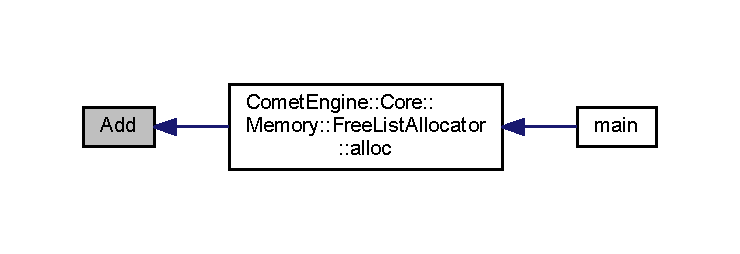
\includegraphics[width=350pt]{namespace_comet_engine_1_1_core_1_1_memory_1_1_utils_a93ae170a43dac9da0116187242b35a6f_icgraph}
\end{center}
\end{figure}
\mbox{\Hypertarget{namespace_comet_engine_1_1_core_1_1_memory_1_1_utils_a893da9f083981a41e4ada733c3d0661f}\label{namespace_comet_engine_1_1_core_1_1_memory_1_1_utils_a893da9f083981a41e4ada733c3d0661f}} 
\index{Comet\+Engine\+::\+Core\+::\+Memory\+::\+Utils@{Comet\+Engine\+::\+Core\+::\+Memory\+::\+Utils}!align\+Forward@{align\+Forward}}
\index{align\+Forward@{align\+Forward}!Comet\+Engine\+::\+Core\+::\+Memory\+::\+Utils@{Comet\+Engine\+::\+Core\+::\+Memory\+::\+Utils}}
\subsubsection{\texorpdfstring{align\+Forward()}{alignForward()}}
{\footnotesize\ttfamily const void $\ast$ align\+Forward (\begin{DoxyParamCaption}\item[{const void $\ast$}]{i\+\_\+base\+\_\+adress,  }\item[{\hyperlink{namespace_comet_engine_1_1_type_aeb22ad46de677e9a50679dfebeb0e6f0}{Type\+::ptr}}]{i\+\_\+alignment }\end{DoxyParamCaption})}



Comet\+Engine\+Memory.\+cpp 파일의 5 번째 라인에서 정의되었습니다.


\begin{DoxyCode}
6 \{
7     \textcolor{keywordflow}{return} (\textcolor{keywordtype}{void}*)(((\hyperlink{namespace_comet_engine_1_1_type_aeb22ad46de677e9a50679dfebeb0e6f0}{Type::ptr})i\_base\_adress) + ((i\_alignment - 1) & (~(i\_alignment - 1))));
8 \}
\end{DoxyCode}
\mbox{\Hypertarget{namespace_comet_engine_1_1_core_1_1_memory_1_1_utils_aa5a0140d498d631a747be87791063f2d}\label{namespace_comet_engine_1_1_core_1_1_memory_1_1_utils_aa5a0140d498d631a747be87791063f2d}} 
\index{Comet\+Engine\+::\+Core\+::\+Memory\+::\+Utils@{Comet\+Engine\+::\+Core\+::\+Memory\+::\+Utils}!align\+Forward\+Adjustment@{align\+Forward\+Adjustment}}
\index{align\+Forward\+Adjustment@{align\+Forward\+Adjustment}!Comet\+Engine\+::\+Core\+::\+Memory\+::\+Utils@{Comet\+Engine\+::\+Core\+::\+Memory\+::\+Utils}}
\subsubsection{\texorpdfstring{align\+Forward\+Adjustment()}{alignForwardAdjustment()}}
{\footnotesize\ttfamily const \hyperlink{namespace_comet_engine_1_1_type_ada4c95a4173a4bb540c8a7f80f3665d2}{Type\+::uint32} align\+Forward\+Adjustment (\begin{DoxyParamCaption}\item[{const void $\ast$}]{i\+\_\+adress,  }\item[{\hyperlink{namespace_comet_engine_1_1_type_aeb22ad46de677e9a50679dfebeb0e6f0}{Type\+::ptr}}]{i\+\_\+alignment }\end{DoxyParamCaption})}



Comet\+Engine\+Memory.\+cpp 파일의 10 번째 라인에서 정의되었습니다.


\begin{DoxyCode}
11 \{
12     \hyperlink{namespace_comet_engine_1_1_type_a1b09856a6463f2bcc4bd8ff0e4e3ee0f}{Type::uint8} adjustment = i\_alignment - ((\hyperlink{namespace_comet_engine_1_1_type_aeb22ad46de677e9a50679dfebeb0e6f0}{Type::ptr})(i\_adress)) & ((
      \hyperlink{namespace_comet_engine_1_1_type_aeb22ad46de677e9a50679dfebeb0e6f0}{Type::ptr}) i\_alignment - 1);
13     \textcolor{keywordflow}{if} (i\_alignment == adjustment)
14         \textcolor{keywordflow}{return} 0;
15     \textcolor{keywordflow}{return} adjustment;
16 \}
\end{DoxyCode}
이 함수를 호출하는 함수들에 대한 그래프입니다.\+:\nopagebreak
\begin{figure}[H]
\begin{center}
\leavevmode
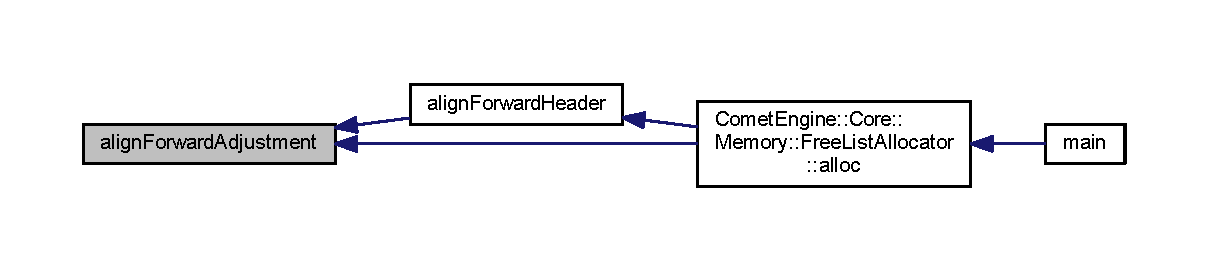
\includegraphics[width=350pt]{namespace_comet_engine_1_1_core_1_1_memory_1_1_utils_aa5a0140d498d631a747be87791063f2d_icgraph}
\end{center}
\end{figure}
\mbox{\Hypertarget{namespace_comet_engine_1_1_core_1_1_memory_1_1_utils_a57bbceefc56fa0e2ec1e472d85ce5e19}\label{namespace_comet_engine_1_1_core_1_1_memory_1_1_utils_a57bbceefc56fa0e2ec1e472d85ce5e19}} 
\index{Comet\+Engine\+::\+Core\+::\+Memory\+::\+Utils@{Comet\+Engine\+::\+Core\+::\+Memory\+::\+Utils}!align\+Forward\+Header@{align\+Forward\+Header}}
\index{align\+Forward\+Header@{align\+Forward\+Header}!Comet\+Engine\+::\+Core\+::\+Memory\+::\+Utils@{Comet\+Engine\+::\+Core\+::\+Memory\+::\+Utils}}
\subsubsection{\texorpdfstring{align\+Forward\+Header()}{alignForwardHeader()}}
{\footnotesize\ttfamily const \hyperlink{namespace_comet_engine_1_1_type_ada4c95a4173a4bb540c8a7f80f3665d2}{Type\+::uint32} align\+Forward\+Header (\begin{DoxyParamCaption}\item[{const void $\ast$}]{i\+\_\+adress,  }\item[{\hyperlink{namespace_comet_engine_1_1_type_aeb22ad46de677e9a50679dfebeb0e6f0}{Type\+::ptr}}]{i\+\_\+alignment,  }\item[{\hyperlink{namespace_comet_engine_1_1_type_ada4c95a4173a4bb540c8a7f80f3665d2}{Type\+::uint32}}]{i\+\_\+\+Header\+Size }\end{DoxyParamCaption})}



Comet\+Engine\+Memory.\+cpp 파일의 18 번째 라인에서 정의되었습니다.


\begin{DoxyCode}
19 \{
20     \hyperlink{namespace_comet_engine_1_1_type_a1b09856a6463f2bcc4bd8ff0e4e3ee0f}{Type::uint8} adjustment = \hyperlink{namespace_comet_engine_1_1_core_1_1_memory_1_1_utils_aa5a0140d498d631a747be87791063f2d}{alignForwardAdjustment}(i\_adress, i\_alignment)
      ;
21     \hyperlink{namespace_comet_engine_1_1_type_a1b09856a6463f2bcc4bd8ff0e4e3ee0f}{Type::uint8} need = i\_HeaderSize;
22     \textcolor{keywordflow}{if} (adjustment < need)
23     \{
24         need -= adjustment;
25         adjustment += i\_alignment* (need / i\_alignment);
26         \textcolor{keywordflow}{if} (need % i\_alignment > 0)
27             adjustment += i\_alignment;
28         \textcolor{keywordflow}{return} adjustment;
29     \}
30 
31 \}
\end{DoxyCode}
이 함수 내부에서 호출하는 함수들에 대한 그래프입니다.\+:\nopagebreak
\begin{figure}[H]
\begin{center}
\leavevmode
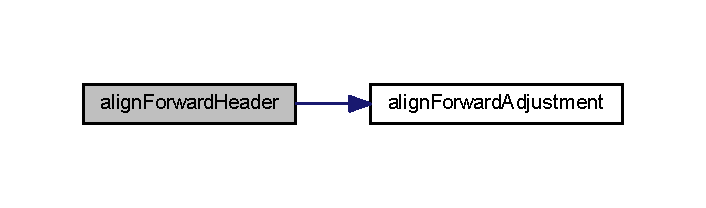
\includegraphics[width=339pt]{namespace_comet_engine_1_1_core_1_1_memory_1_1_utils_a57bbceefc56fa0e2ec1e472d85ce5e19_cgraph}
\end{center}
\end{figure}
이 함수를 호출하는 함수들에 대한 그래프입니다.\+:\nopagebreak
\begin{figure}[H]
\begin{center}
\leavevmode
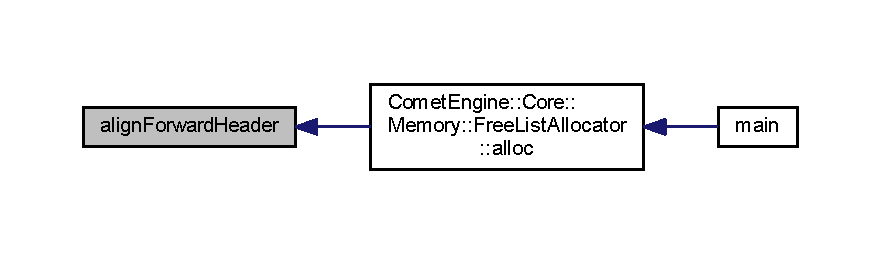
\includegraphics[width=350pt]{namespace_comet_engine_1_1_core_1_1_memory_1_1_utils_a57bbceefc56fa0e2ec1e472d85ce5e19_icgraph}
\end{center}
\end{figure}
\mbox{\Hypertarget{namespace_comet_engine_1_1_core_1_1_memory_1_1_utils_a4e360b8988f0de099daa987e3b5f09ed}\label{namespace_comet_engine_1_1_core_1_1_memory_1_1_utils_a4e360b8988f0de099daa987e3b5f09ed}} 
\index{Comet\+Engine\+::\+Core\+::\+Memory\+::\+Utils@{Comet\+Engine\+::\+Core\+::\+Memory\+::\+Utils}!Sub@{Sub}}
\index{Sub@{Sub}!Comet\+Engine\+::\+Core\+::\+Memory\+::\+Utils@{Comet\+Engine\+::\+Core\+::\+Memory\+::\+Utils}}
\subsubsection{\texorpdfstring{Sub()}{Sub()}}
{\footnotesize\ttfamily const void $\ast$ Sub (\begin{DoxyParamCaption}\item[{const void $\ast$}]{A,  }\item[{const void $\ast$}]{B }\end{DoxyParamCaption})}



Comet\+Engine\+Memory.\+cpp 파일의 38 번째 라인에서 정의되었습니다.


\begin{DoxyCode}
39 \{
40     \textcolor{keywordflow}{return} (\textcolor{keywordtype}{void}*)((\hyperlink{namespace_comet_engine_1_1_type_aeb22ad46de677e9a50679dfebeb0e6f0}{Type::ptr})A - (\hyperlink{namespace_comet_engine_1_1_type_aeb22ad46de677e9a50679dfebeb0e6f0}{Type::ptr})B);
41 \}
\end{DoxyCode}
이 함수를 호출하는 함수들에 대한 그래프입니다.\+:\nopagebreak
\begin{figure}[H]
\begin{center}
\leavevmode
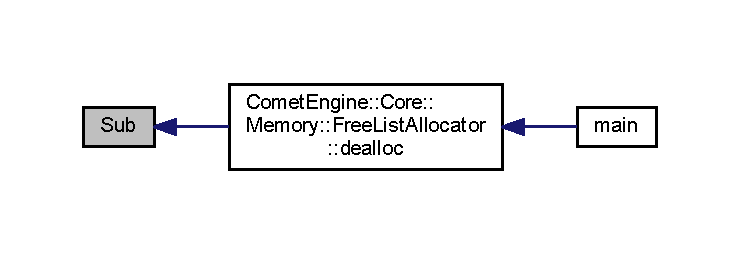
\includegraphics[width=350pt]{namespace_comet_engine_1_1_core_1_1_memory_1_1_utils_a4e360b8988f0de099daa987e3b5f09ed_icgraph}
\end{center}
\end{figure}

\hypertarget{namespace_comet_engine_1_1_renderer}{}\section{Comet\+Engine\+:\+:Renderer 네임스페이스 참조}
\label{namespace_comet_engine_1_1_renderer}\index{Comet\+Engine\+::\+Renderer@{Comet\+Engine\+::\+Renderer}}
\subsection*{클래스}
\begin{DoxyCompactItemize}
\item 
class \hyperlink{class_comet_engine_1_1_renderer_1_1_comet_engine_d_x_renderer}{Comet\+Engine\+D\+X\+Renderer}
\end{DoxyCompactItemize}

\hypertarget{namespace_comet_engine_1_1_type}{}\section{Comet\+Engine\+:\+:Type 네임스페이스 참조}
\label{namespace_comet_engine_1_1_type}\index{Comet\+Engine\+::\+Type@{Comet\+Engine\+::\+Type}}
\subsection*{타입정의}
\begin{DoxyCompactItemize}
\item 
typedef unsigned int \hyperlink{namespace_comet_engine_1_1_type_a7c94ea6f8948649f8d181ae55911eeaf}{size\+\_\+t}
\item 
typedef unsigned long \hyperlink{namespace_comet_engine_1_1_type_aeb22ad46de677e9a50679dfebeb0e6f0}{ptr}
\item 
typedef \+\_\+\+\_\+int8 \hyperlink{namespace_comet_engine_1_1_type_aaf44e46c719bc25ff3de1341e7aa4094}{int8}
\item 
typedef \+\_\+\+\_\+int32 \hyperlink{namespace_comet_engine_1_1_type_ad3ce9f24199b79b2629169eebf59489b}{int32}
\item 
typedef \+\_\+\+\_\+int64 \hyperlink{namespace_comet_engine_1_1_type_a92a47ab0e245f0ae4d01c38a64b6c427}{int64}
\item 
typedef unsigned \+\_\+\+\_\+int8 \hyperlink{namespace_comet_engine_1_1_type_a1b09856a6463f2bcc4bd8ff0e4e3ee0f}{uint8}
\item 
typedef unsigned \+\_\+\+\_\+int32 \hyperlink{namespace_comet_engine_1_1_type_ada4c95a4173a4bb540c8a7f80f3665d2}{uint32}
\item 
typedef unsigned int \hyperlink{namespace_comet_engine_1_1_type_a91ad9478d81a7aaf2593e8d9c3d06a14}{uint}
\item 
typedef unsigned \+\_\+\+\_\+int64 \hyperlink{namespace_comet_engine_1_1_type_ac6afe794ed283c11fb63426a58188e5e}{uint64}
\end{DoxyCompactItemize}


\subsection{타입정의 문서화}
\mbox{\Hypertarget{namespace_comet_engine_1_1_type_ad3ce9f24199b79b2629169eebf59489b}\label{namespace_comet_engine_1_1_type_ad3ce9f24199b79b2629169eebf59489b}} 
\index{Comet\+Engine\+::\+Type@{Comet\+Engine\+::\+Type}!int32@{int32}}
\index{int32@{int32}!Comet\+Engine\+::\+Type@{Comet\+Engine\+::\+Type}}
\subsubsection{\texorpdfstring{int32}{int32}}
{\footnotesize\ttfamily typedef \+\_\+\+\_\+int32 \hyperlink{namespace_comet_engine_1_1_type_ad3ce9f24199b79b2629169eebf59489b}{int32}}



Comet\+Engine\+Types.\+h 파일의 22 번째 라인에서 정의되었습니다.

\mbox{\Hypertarget{namespace_comet_engine_1_1_type_a92a47ab0e245f0ae4d01c38a64b6c427}\label{namespace_comet_engine_1_1_type_a92a47ab0e245f0ae4d01c38a64b6c427}} 
\index{Comet\+Engine\+::\+Type@{Comet\+Engine\+::\+Type}!int64@{int64}}
\index{int64@{int64}!Comet\+Engine\+::\+Type@{Comet\+Engine\+::\+Type}}
\subsubsection{\texorpdfstring{int64}{int64}}
{\footnotesize\ttfamily typedef \+\_\+\+\_\+int64 \hyperlink{namespace_comet_engine_1_1_type_a92a47ab0e245f0ae4d01c38a64b6c427}{int64}}



Comet\+Engine\+Types.\+h 파일의 23 번째 라인에서 정의되었습니다.

\mbox{\Hypertarget{namespace_comet_engine_1_1_type_aaf44e46c719bc25ff3de1341e7aa4094}\label{namespace_comet_engine_1_1_type_aaf44e46c719bc25ff3de1341e7aa4094}} 
\index{Comet\+Engine\+::\+Type@{Comet\+Engine\+::\+Type}!int8@{int8}}
\index{int8@{int8}!Comet\+Engine\+::\+Type@{Comet\+Engine\+::\+Type}}
\subsubsection{\texorpdfstring{int8}{int8}}
{\footnotesize\ttfamily typedef \+\_\+\+\_\+int8 \hyperlink{namespace_comet_engine_1_1_type_aaf44e46c719bc25ff3de1341e7aa4094}{int8}}



Comet\+Engine\+Types.\+h 파일의 21 번째 라인에서 정의되었습니다.

\mbox{\Hypertarget{namespace_comet_engine_1_1_type_aeb22ad46de677e9a50679dfebeb0e6f0}\label{namespace_comet_engine_1_1_type_aeb22ad46de677e9a50679dfebeb0e6f0}} 
\index{Comet\+Engine\+::\+Type@{Comet\+Engine\+::\+Type}!ptr@{ptr}}
\index{ptr@{ptr}!Comet\+Engine\+::\+Type@{Comet\+Engine\+::\+Type}}
\subsubsection{\texorpdfstring{ptr}{ptr}}
{\footnotesize\ttfamily typedef unsigned long \hyperlink{namespace_comet_engine_1_1_type_aeb22ad46de677e9a50679dfebeb0e6f0}{ptr}}



Comet\+Engine\+Types.\+h 파일의 18 번째 라인에서 정의되었습니다.

\mbox{\Hypertarget{namespace_comet_engine_1_1_type_a7c94ea6f8948649f8d181ae55911eeaf}\label{namespace_comet_engine_1_1_type_a7c94ea6f8948649f8d181ae55911eeaf}} 
\index{Comet\+Engine\+::\+Type@{Comet\+Engine\+::\+Type}!size\+\_\+t@{size\+\_\+t}}
\index{size\+\_\+t@{size\+\_\+t}!Comet\+Engine\+::\+Type@{Comet\+Engine\+::\+Type}}
\subsubsection{\texorpdfstring{size\+\_\+t}{size\_t}}
{\footnotesize\ttfamily typedef unsigned int \hyperlink{namespace_comet_engine_1_1_type_a7c94ea6f8948649f8d181ae55911eeaf}{size\+\_\+t}}



Comet\+Engine\+Types.\+h 파일의 17 번째 라인에서 정의되었습니다.

\mbox{\Hypertarget{namespace_comet_engine_1_1_type_a91ad9478d81a7aaf2593e8d9c3d06a14}\label{namespace_comet_engine_1_1_type_a91ad9478d81a7aaf2593e8d9c3d06a14}} 
\index{Comet\+Engine\+::\+Type@{Comet\+Engine\+::\+Type}!uint@{uint}}
\index{uint@{uint}!Comet\+Engine\+::\+Type@{Comet\+Engine\+::\+Type}}
\subsubsection{\texorpdfstring{uint}{uint}}
{\footnotesize\ttfamily typedef unsigned int \hyperlink{namespace_comet_engine_1_1_type_a91ad9478d81a7aaf2593e8d9c3d06a14}{uint}}



Comet\+Engine\+Types.\+h 파일의 27 번째 라인에서 정의되었습니다.

\mbox{\Hypertarget{namespace_comet_engine_1_1_type_ada4c95a4173a4bb540c8a7f80f3665d2}\label{namespace_comet_engine_1_1_type_ada4c95a4173a4bb540c8a7f80f3665d2}} 
\index{Comet\+Engine\+::\+Type@{Comet\+Engine\+::\+Type}!uint32@{uint32}}
\index{uint32@{uint32}!Comet\+Engine\+::\+Type@{Comet\+Engine\+::\+Type}}
\subsubsection{\texorpdfstring{uint32}{uint32}}
{\footnotesize\ttfamily typedef unsigned \+\_\+\+\_\+int32 \hyperlink{namespace_comet_engine_1_1_type_ada4c95a4173a4bb540c8a7f80f3665d2}{uint32}}



Comet\+Engine\+Types.\+h 파일의 26 번째 라인에서 정의되었습니다.

\mbox{\Hypertarget{namespace_comet_engine_1_1_type_ac6afe794ed283c11fb63426a58188e5e}\label{namespace_comet_engine_1_1_type_ac6afe794ed283c11fb63426a58188e5e}} 
\index{Comet\+Engine\+::\+Type@{Comet\+Engine\+::\+Type}!uint64@{uint64}}
\index{uint64@{uint64}!Comet\+Engine\+::\+Type@{Comet\+Engine\+::\+Type}}
\subsubsection{\texorpdfstring{uint64}{uint64}}
{\footnotesize\ttfamily typedef unsigned \+\_\+\+\_\+int64 \hyperlink{namespace_comet_engine_1_1_type_ac6afe794ed283c11fb63426a58188e5e}{uint64}}



Comet\+Engine\+Types.\+h 파일의 28 번째 라인에서 정의되었습니다.

\mbox{\Hypertarget{namespace_comet_engine_1_1_type_a1b09856a6463f2bcc4bd8ff0e4e3ee0f}\label{namespace_comet_engine_1_1_type_a1b09856a6463f2bcc4bd8ff0e4e3ee0f}} 
\index{Comet\+Engine\+::\+Type@{Comet\+Engine\+::\+Type}!uint8@{uint8}}
\index{uint8@{uint8}!Comet\+Engine\+::\+Type@{Comet\+Engine\+::\+Type}}
\subsubsection{\texorpdfstring{uint8}{uint8}}
{\footnotesize\ttfamily typedef unsigned \+\_\+\+\_\+int8 \hyperlink{namespace_comet_engine_1_1_type_a1b09856a6463f2bcc4bd8ff0e4e3ee0f}{uint8}}



Comet\+Engine\+Types.\+h 파일의 25 번째 라인에서 정의되었습니다.


\hypertarget{namespace_comet_engine_tester}{}\section{Comet\+Engine\+Tester 네임스페이스 참조}
\label{namespace_comet_engine_tester}\index{Comet\+Engine\+Tester@{Comet\+Engine\+Tester}}
\subsection*{클래스}
\begin{DoxyCompactItemize}
\item 
class \hyperlink{class_comet_engine_tester_1_1_program}{Program}
\end{DoxyCompactItemize}

\chapter{클래스 문서화}
\hypertarget{class_comet_engine_1_1_core_1_1_memory_1_1_base_allocator}{}\section{Base\+Allocator 클래스 참조}
\label{class_comet_engine_1_1_core_1_1_memory_1_1_base_allocator}\index{Base\+Allocator@{Base\+Allocator}}


{\ttfamily \#include $<$Comet\+Engine\+Memory.\+h$>$}



Base\+Allocator에 대한 상속 다이어그램 \+: 
\nopagebreak
\begin{figure}[H]
\begin{center}
\leavevmode
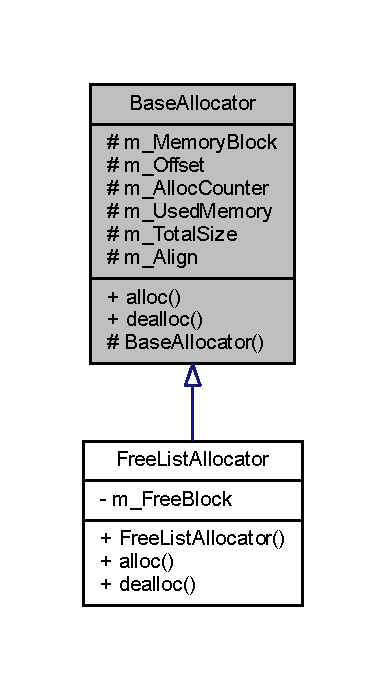
\includegraphics[width=185pt]{class_comet_engine_1_1_core_1_1_memory_1_1_base_allocator__inherit__graph}
\end{center}
\end{figure}


Base\+Allocator에 대한 협력 다이어그램\+:\nopagebreak
\begin{figure}[H]
\begin{center}
\leavevmode
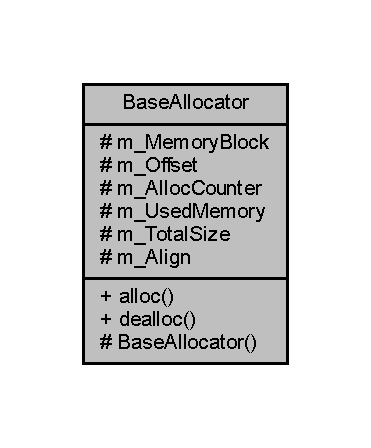
\includegraphics[width=178pt]{class_comet_engine_1_1_core_1_1_memory_1_1_base_allocator__coll__graph}
\end{center}
\end{figure}
\subsection*{Public 멤버 함수}
\begin{DoxyCompactItemize}
\item 
virtual void $\ast$ \hyperlink{class_comet_engine_1_1_core_1_1_memory_1_1_base_allocator_a8f51b4daa12e31477f57003494c09098}{alloc} (\hyperlink{namespace_comet_engine_1_1_type_a7c94ea6f8948649f8d181ae55911eeaf}{Type\+::size\+\_\+t} i\+\_\+byte)=0
\item 
virtual void \hyperlink{class_comet_engine_1_1_core_1_1_memory_1_1_base_allocator_acca0d1592319cfecb53f8333033a644b}{dealloc} (void $\ast$i\+\_\+\+Adress)=0
\end{DoxyCompactItemize}
\subsection*{Protected 멤버 함수}
\begin{DoxyCompactItemize}
\item 
\hyperlink{class_comet_engine_1_1_core_1_1_memory_1_1_base_allocator_a389c24863a5abee333f325634c18bea3}{Base\+Allocator} (void $\ast$i\+\_\+\+Memory\+Block, \hyperlink{namespace_comet_engine_1_1_type_a1b09856a6463f2bcc4bd8ff0e4e3ee0f}{Type\+::uint8} i\+\_\+align, \hyperlink{namespace_comet_engine_1_1_type_a7c94ea6f8948649f8d181ae55911eeaf}{Type\+::size\+\_\+t} i\+\_\+\+Memory\+Size, \hyperlink{namespace_comet_engine_1_1_type_a7c94ea6f8948649f8d181ae55911eeaf}{Type\+::size\+\_\+t} i\+\_\+offset=0)
\end{DoxyCompactItemize}
\subsection*{Protected 속성}
\begin{DoxyCompactItemize}
\item 
void $\ast$ \hyperlink{class_comet_engine_1_1_core_1_1_memory_1_1_base_allocator_a24b4bdf45e7f4b6109b6d1cc455c6f26}{m\+\_\+\+Memory\+Block}
\item 
\hyperlink{namespace_comet_engine_1_1_type_a7c94ea6f8948649f8d181ae55911eeaf}{Type\+::size\+\_\+t} \hyperlink{class_comet_engine_1_1_core_1_1_memory_1_1_base_allocator_a71e2142fb28745ce9bc64de3a0ea1956}{m\+\_\+\+Offset}
\item 
\hyperlink{namespace_comet_engine_1_1_type_a7c94ea6f8948649f8d181ae55911eeaf}{Type\+::size\+\_\+t} \hyperlink{class_comet_engine_1_1_core_1_1_memory_1_1_base_allocator_abed7f06b465ee178701fe2cfc1aff9a6}{m\+\_\+\+Alloc\+Counter}
\item 
\hyperlink{namespace_comet_engine_1_1_type_a7c94ea6f8948649f8d181ae55911eeaf}{Type\+::size\+\_\+t} \hyperlink{class_comet_engine_1_1_core_1_1_memory_1_1_base_allocator_a1420047b91508f9ab33c448e8371511c}{m\+\_\+\+Used\+Memory}
\item 
\hyperlink{namespace_comet_engine_1_1_type_a7c94ea6f8948649f8d181ae55911eeaf}{Type\+::size\+\_\+t} \hyperlink{class_comet_engine_1_1_core_1_1_memory_1_1_base_allocator_abba9914681f05b98a55770daaf7d94be}{m\+\_\+\+Total\+Size}
\item 
\hyperlink{namespace_comet_engine_1_1_type_a1b09856a6463f2bcc4bd8ff0e4e3ee0f}{Type\+::uint8} \hyperlink{class_comet_engine_1_1_core_1_1_memory_1_1_base_allocator_a01f973630e3c1ac98b9defda193793b8}{m\+\_\+\+Align}
\end{DoxyCompactItemize}


\subsection{상세한 설명}


Comet\+Engine\+Memory.\+h 파일의 51 번째 라인에서 정의되었습니다.



\subsection{생성자 \& 소멸자 문서화}
\mbox{\Hypertarget{class_comet_engine_1_1_core_1_1_memory_1_1_base_allocator_a389c24863a5abee333f325634c18bea3}\label{class_comet_engine_1_1_core_1_1_memory_1_1_base_allocator_a389c24863a5abee333f325634c18bea3}} 
\index{Comet\+Engine\+::\+Core\+::\+Memory\+::\+Base\+Allocator@{Comet\+Engine\+::\+Core\+::\+Memory\+::\+Base\+Allocator}!Base\+Allocator@{Base\+Allocator}}
\index{Base\+Allocator@{Base\+Allocator}!Comet\+Engine\+::\+Core\+::\+Memory\+::\+Base\+Allocator@{Comet\+Engine\+::\+Core\+::\+Memory\+::\+Base\+Allocator}}
\subsubsection{\texorpdfstring{Base\+Allocator()}{BaseAllocator()}}
{\footnotesize\ttfamily \hyperlink{class_comet_engine_1_1_core_1_1_memory_1_1_base_allocator}{Base\+Allocator} (\begin{DoxyParamCaption}\item[{void $\ast$}]{i\+\_\+\+Memory\+Block,  }\item[{\hyperlink{namespace_comet_engine_1_1_type_a1b09856a6463f2bcc4bd8ff0e4e3ee0f}{Type\+::uint8}}]{i\+\_\+align,  }\item[{\hyperlink{namespace_comet_engine_1_1_type_a7c94ea6f8948649f8d181ae55911eeaf}{Type\+::size\+\_\+t}}]{i\+\_\+\+Memory\+Size,  }\item[{\hyperlink{namespace_comet_engine_1_1_type_a7c94ea6f8948649f8d181ae55911eeaf}{Type\+::size\+\_\+t}}]{i\+\_\+offset = {\ttfamily 0} }\end{DoxyParamCaption})\hspace{0.3cm}{\ttfamily [protected]}}



Comet\+Engine\+Memory.\+cpp 파일의 43 번째 라인에서 정의되었습니다.


\begin{DoxyCode}
44 \{
45     \hyperlink{class_comet_engine_1_1_core_1_1_memory_1_1_base_allocator_a71e2142fb28745ce9bc64de3a0ea1956}{m\_Offset} = i\_offset;
46     \hyperlink{class_comet_engine_1_1_core_1_1_memory_1_1_base_allocator_a24b4bdf45e7f4b6109b6d1cc455c6f26}{m\_MemoryBlock} = (\textcolor{keywordtype}{void}*)((\hyperlink{namespace_comet_engine_1_1_type_aeb22ad46de677e9a50679dfebeb0e6f0}{Type::ptr})i\_MemoryBlock + (
      \hyperlink{namespace_comet_engine_1_1_type_aeb22ad46de677e9a50679dfebeb0e6f0}{Type::ptr})i\_offset);
47     \hyperlink{class_comet_engine_1_1_core_1_1_memory_1_1_base_allocator_abba9914681f05b98a55770daaf7d94be}{m\_TotalSize} = i\_MemorySize;
48     \hyperlink{class_comet_engine_1_1_core_1_1_memory_1_1_base_allocator_a01f973630e3c1ac98b9defda193793b8}{m\_Align} = i\_align;
49     \hyperlink{class_comet_engine_1_1_core_1_1_memory_1_1_base_allocator_abed7f06b465ee178701fe2cfc1aff9a6}{m\_AllocCounter} = 0;
50     \hyperlink{class_comet_engine_1_1_core_1_1_memory_1_1_base_allocator_a1420047b91508f9ab33c448e8371511c}{m\_UsedMemory} = 0;
51 
52 \}
\end{DoxyCode}


\subsection{멤버 함수 문서화}
\mbox{\Hypertarget{class_comet_engine_1_1_core_1_1_memory_1_1_base_allocator_a8f51b4daa12e31477f57003494c09098}\label{class_comet_engine_1_1_core_1_1_memory_1_1_base_allocator_a8f51b4daa12e31477f57003494c09098}} 
\index{Comet\+Engine\+::\+Core\+::\+Memory\+::\+Base\+Allocator@{Comet\+Engine\+::\+Core\+::\+Memory\+::\+Base\+Allocator}!alloc@{alloc}}
\index{alloc@{alloc}!Comet\+Engine\+::\+Core\+::\+Memory\+::\+Base\+Allocator@{Comet\+Engine\+::\+Core\+::\+Memory\+::\+Base\+Allocator}}
\subsubsection{\texorpdfstring{alloc()}{alloc()}}
{\footnotesize\ttfamily virtual void$\ast$ alloc (\begin{DoxyParamCaption}\item[{\hyperlink{namespace_comet_engine_1_1_type_a7c94ea6f8948649f8d181ae55911eeaf}{Type\+::size\+\_\+t}}]{i\+\_\+byte }\end{DoxyParamCaption})\hspace{0.3cm}{\ttfamily [pure virtual]}}



\hyperlink{class_comet_engine_1_1_core_1_1_memory_1_1_free_list_allocator_a73ff0a374ba86a2c447aaf05ad04e932}{Free\+List\+Allocator}에서 구현되었습니다.

\mbox{\Hypertarget{class_comet_engine_1_1_core_1_1_memory_1_1_base_allocator_acca0d1592319cfecb53f8333033a644b}\label{class_comet_engine_1_1_core_1_1_memory_1_1_base_allocator_acca0d1592319cfecb53f8333033a644b}} 
\index{Comet\+Engine\+::\+Core\+::\+Memory\+::\+Base\+Allocator@{Comet\+Engine\+::\+Core\+::\+Memory\+::\+Base\+Allocator}!dealloc@{dealloc}}
\index{dealloc@{dealloc}!Comet\+Engine\+::\+Core\+::\+Memory\+::\+Base\+Allocator@{Comet\+Engine\+::\+Core\+::\+Memory\+::\+Base\+Allocator}}
\subsubsection{\texorpdfstring{dealloc()}{dealloc()}}
{\footnotesize\ttfamily virtual void dealloc (\begin{DoxyParamCaption}\item[{void $\ast$}]{i\+\_\+\+Adress }\end{DoxyParamCaption})\hspace{0.3cm}{\ttfamily [pure virtual]}}



\hyperlink{class_comet_engine_1_1_core_1_1_memory_1_1_free_list_allocator_ab7a97e4b1500c7ef2c2edc3bec28a84f}{Free\+List\+Allocator}에서 구현되었습니다.



\subsection{멤버 데이터 문서화}
\mbox{\Hypertarget{class_comet_engine_1_1_core_1_1_memory_1_1_base_allocator_a01f973630e3c1ac98b9defda193793b8}\label{class_comet_engine_1_1_core_1_1_memory_1_1_base_allocator_a01f973630e3c1ac98b9defda193793b8}} 
\index{Comet\+Engine\+::\+Core\+::\+Memory\+::\+Base\+Allocator@{Comet\+Engine\+::\+Core\+::\+Memory\+::\+Base\+Allocator}!m\+\_\+\+Align@{m\+\_\+\+Align}}
\index{m\+\_\+\+Align@{m\+\_\+\+Align}!Comet\+Engine\+::\+Core\+::\+Memory\+::\+Base\+Allocator@{Comet\+Engine\+::\+Core\+::\+Memory\+::\+Base\+Allocator}}
\subsubsection{\texorpdfstring{m\+\_\+\+Align}{m\_Align}}
{\footnotesize\ttfamily \hyperlink{namespace_comet_engine_1_1_type_a1b09856a6463f2bcc4bd8ff0e4e3ee0f}{Type\+::uint8} m\+\_\+\+Align\hspace{0.3cm}{\ttfamily [protected]}}



Comet\+Engine\+Memory.\+h 파일의 59 번째 라인에서 정의되었습니다.

\mbox{\Hypertarget{class_comet_engine_1_1_core_1_1_memory_1_1_base_allocator_abed7f06b465ee178701fe2cfc1aff9a6}\label{class_comet_engine_1_1_core_1_1_memory_1_1_base_allocator_abed7f06b465ee178701fe2cfc1aff9a6}} 
\index{Comet\+Engine\+::\+Core\+::\+Memory\+::\+Base\+Allocator@{Comet\+Engine\+::\+Core\+::\+Memory\+::\+Base\+Allocator}!m\+\_\+\+Alloc\+Counter@{m\+\_\+\+Alloc\+Counter}}
\index{m\+\_\+\+Alloc\+Counter@{m\+\_\+\+Alloc\+Counter}!Comet\+Engine\+::\+Core\+::\+Memory\+::\+Base\+Allocator@{Comet\+Engine\+::\+Core\+::\+Memory\+::\+Base\+Allocator}}
\subsubsection{\texorpdfstring{m\+\_\+\+Alloc\+Counter}{m\_AllocCounter}}
{\footnotesize\ttfamily \hyperlink{namespace_comet_engine_1_1_type_a7c94ea6f8948649f8d181ae55911eeaf}{Type\+::size\+\_\+t} m\+\_\+\+Alloc\+Counter\hspace{0.3cm}{\ttfamily [protected]}}



Comet\+Engine\+Memory.\+h 파일의 56 번째 라인에서 정의되었습니다.

\mbox{\Hypertarget{class_comet_engine_1_1_core_1_1_memory_1_1_base_allocator_a24b4bdf45e7f4b6109b6d1cc455c6f26}\label{class_comet_engine_1_1_core_1_1_memory_1_1_base_allocator_a24b4bdf45e7f4b6109b6d1cc455c6f26}} 
\index{Comet\+Engine\+::\+Core\+::\+Memory\+::\+Base\+Allocator@{Comet\+Engine\+::\+Core\+::\+Memory\+::\+Base\+Allocator}!m\+\_\+\+Memory\+Block@{m\+\_\+\+Memory\+Block}}
\index{m\+\_\+\+Memory\+Block@{m\+\_\+\+Memory\+Block}!Comet\+Engine\+::\+Core\+::\+Memory\+::\+Base\+Allocator@{Comet\+Engine\+::\+Core\+::\+Memory\+::\+Base\+Allocator}}
\subsubsection{\texorpdfstring{m\+\_\+\+Memory\+Block}{m\_MemoryBlock}}
{\footnotesize\ttfamily void$\ast$ m\+\_\+\+Memory\+Block\hspace{0.3cm}{\ttfamily [protected]}}



Comet\+Engine\+Memory.\+h 파일의 54 번째 라인에서 정의되었습니다.

\mbox{\Hypertarget{class_comet_engine_1_1_core_1_1_memory_1_1_base_allocator_a71e2142fb28745ce9bc64de3a0ea1956}\label{class_comet_engine_1_1_core_1_1_memory_1_1_base_allocator_a71e2142fb28745ce9bc64de3a0ea1956}} 
\index{Comet\+Engine\+::\+Core\+::\+Memory\+::\+Base\+Allocator@{Comet\+Engine\+::\+Core\+::\+Memory\+::\+Base\+Allocator}!m\+\_\+\+Offset@{m\+\_\+\+Offset}}
\index{m\+\_\+\+Offset@{m\+\_\+\+Offset}!Comet\+Engine\+::\+Core\+::\+Memory\+::\+Base\+Allocator@{Comet\+Engine\+::\+Core\+::\+Memory\+::\+Base\+Allocator}}
\subsubsection{\texorpdfstring{m\+\_\+\+Offset}{m\_Offset}}
{\footnotesize\ttfamily \hyperlink{namespace_comet_engine_1_1_type_a7c94ea6f8948649f8d181ae55911eeaf}{Type\+::size\+\_\+t} m\+\_\+\+Offset\hspace{0.3cm}{\ttfamily [protected]}}



Comet\+Engine\+Memory.\+h 파일의 55 번째 라인에서 정의되었습니다.

\mbox{\Hypertarget{class_comet_engine_1_1_core_1_1_memory_1_1_base_allocator_abba9914681f05b98a55770daaf7d94be}\label{class_comet_engine_1_1_core_1_1_memory_1_1_base_allocator_abba9914681f05b98a55770daaf7d94be}} 
\index{Comet\+Engine\+::\+Core\+::\+Memory\+::\+Base\+Allocator@{Comet\+Engine\+::\+Core\+::\+Memory\+::\+Base\+Allocator}!m\+\_\+\+Total\+Size@{m\+\_\+\+Total\+Size}}
\index{m\+\_\+\+Total\+Size@{m\+\_\+\+Total\+Size}!Comet\+Engine\+::\+Core\+::\+Memory\+::\+Base\+Allocator@{Comet\+Engine\+::\+Core\+::\+Memory\+::\+Base\+Allocator}}
\subsubsection{\texorpdfstring{m\+\_\+\+Total\+Size}{m\_TotalSize}}
{\footnotesize\ttfamily \hyperlink{namespace_comet_engine_1_1_type_a7c94ea6f8948649f8d181ae55911eeaf}{Type\+::size\+\_\+t} m\+\_\+\+Total\+Size\hspace{0.3cm}{\ttfamily [protected]}}



Comet\+Engine\+Memory.\+h 파일의 58 번째 라인에서 정의되었습니다.

\mbox{\Hypertarget{class_comet_engine_1_1_core_1_1_memory_1_1_base_allocator_a1420047b91508f9ab33c448e8371511c}\label{class_comet_engine_1_1_core_1_1_memory_1_1_base_allocator_a1420047b91508f9ab33c448e8371511c}} 
\index{Comet\+Engine\+::\+Core\+::\+Memory\+::\+Base\+Allocator@{Comet\+Engine\+::\+Core\+::\+Memory\+::\+Base\+Allocator}!m\+\_\+\+Used\+Memory@{m\+\_\+\+Used\+Memory}}
\index{m\+\_\+\+Used\+Memory@{m\+\_\+\+Used\+Memory}!Comet\+Engine\+::\+Core\+::\+Memory\+::\+Base\+Allocator@{Comet\+Engine\+::\+Core\+::\+Memory\+::\+Base\+Allocator}}
\subsubsection{\texorpdfstring{m\+\_\+\+Used\+Memory}{m\_UsedMemory}}
{\footnotesize\ttfamily \hyperlink{namespace_comet_engine_1_1_type_a7c94ea6f8948649f8d181ae55911eeaf}{Type\+::size\+\_\+t} m\+\_\+\+Used\+Memory\hspace{0.3cm}{\ttfamily [protected]}}



Comet\+Engine\+Memory.\+h 파일의 57 번째 라인에서 정의되었습니다.



이 클래스에 대한 문서화 페이지는 다음의 파일들로부터 생성되었습니다.\+:\begin{DoxyCompactItemize}
\item 
Comet\+Engine\+Common/\+Comet\+Engine/\+Comet\+Engine/\+Memory/\hyperlink{_comet_engine_memory_8h}{Comet\+Engine\+Memory.\+h}\item 
Comet\+Engine\+Common/\+Comet\+Engine/\+Comet\+Engine/\+Memory/\hyperlink{_comet_engine_memory_8cpp}{Comet\+Engine\+Memory.\+cpp}\end{DoxyCompactItemize}

\hypertarget{class_comet_engine_1_1_client_1_1_comet_engine_client}{}\section{Comet\+Engine\+Client 클래스 참조}
\label{class_comet_engine_1_1_client_1_1_comet_engine_client}\index{Comet\+Engine\+Client@{Comet\+Engine\+Client}}


Comet\+Engine\+Client에 대한 협력 다이어그램\+:\nopagebreak
\begin{figure}[H]
\begin{center}
\leavevmode
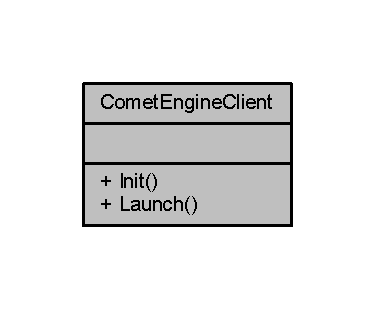
\includegraphics[width=180pt]{class_comet_engine_1_1_client_1_1_comet_engine_client__coll__graph}
\end{center}
\end{figure}
\subsection*{정적 Public 멤버 함수}
\begin{DoxyCompactItemize}
\item 
static bool \hyperlink{class_comet_engine_1_1_client_1_1_comet_engine_client_af5f8db49a5de5bb41cf935066d21f5aa}{Init} (string Window\+Title, int \hyperlink{_d_l_l_comet_engine_win32_8cpp_abbe7749c3b402f7dfe64f936774cfcd4}{Width}, int \hyperlink{_d_l_l_comet_engine_win32_8cpp_afd53bc431b967813e00ae3cfecd5c548}{Height}, \hyperlink{namespace_comet_engine_1_1_client_a608d2e459fd95babca189e50f4182a65}{W\+Indow\+Modes} Display\+Mode, int Render\+Scale, int Msaa\+Level)
\item 
static void \hyperlink{class_comet_engine_1_1_client_1_1_comet_engine_client_aee7b13887a71ba1fcd42c5fbccf124d4}{Launch} ()
\end{DoxyCompactItemize}


\subsection{상세한 설명}


Comet\+Engine\+Client.\+cs 파일의 10 번째 라인에서 정의되었습니다.



\subsection{멤버 함수 문서화}
\mbox{\Hypertarget{class_comet_engine_1_1_client_1_1_comet_engine_client_af5f8db49a5de5bb41cf935066d21f5aa}\label{class_comet_engine_1_1_client_1_1_comet_engine_client_af5f8db49a5de5bb41cf935066d21f5aa}} 
\index{Comet\+Engine\+::\+Client\+::\+Comet\+Engine\+Client@{Comet\+Engine\+::\+Client\+::\+Comet\+Engine\+Client}!Init@{Init}}
\index{Init@{Init}!Comet\+Engine\+::\+Client\+::\+Comet\+Engine\+Client@{Comet\+Engine\+::\+Client\+::\+Comet\+Engine\+Client}}
\subsubsection{\texorpdfstring{Init()}{Init()}}
{\footnotesize\ttfamily static bool Init (\begin{DoxyParamCaption}\item[{string}]{Window\+Title,  }\item[{int}]{Width,  }\item[{int}]{Height,  }\item[{\hyperlink{namespace_comet_engine_1_1_client_a608d2e459fd95babca189e50f4182a65}{W\+Indow\+Modes}}]{Display\+Mode,  }\item[{int}]{Render\+Scale,  }\item[{int}]{Msaa\+Level }\end{DoxyParamCaption})\hspace{0.3cm}{\ttfamily [inline]}, {\ttfamily [static]}}



Comet\+Engine\+Client.\+cs 파일의 14 번째 라인에서 정의되었습니다.


\begin{DoxyCode}
15         \{
16             \textcolor{keywordtype}{bool} SucessFlag =  CometEngineClientWin32.Init(WindowTitle, \hyperlink{_d_l_l_comet_engine_win32_8cpp_abbe7749c3b402f7dfe64f936774cfcd4}{Width}, 
      \hyperlink{_d_l_l_comet_engine_win32_8cpp_afd53bc431b967813e00ae3cfecd5c548}{Height}, DisplayMode,
17                Process.GetCurrentProcess().Handle \textcolor{comment}{/*hInstance*/}, \textcolor{keywordtype}{string}.Empty\textcolor{comment}{/*lpCmdLine*/});
18             \textcolor{keywordflow}{if} (SucessFlag == \textcolor{keyword}{false})
19                \textcolor{keywordflow}{return} \textcolor{keyword}{false};
20 
21             CometEngineDXRenderer.EnableDebugDevice(\textcolor{keyword}{true});
22             SucessFlag = CometEngineDXRenderer.Init(\hyperlink{_d_l_l_comet_engine_win32_8cpp_abbe7749c3b402f7dfe64f936774cfcd4}{Width}, \hyperlink{_d_l_l_comet_engine_win32_8cpp_afd53bc431b967813e00ae3cfecd5c548}{Height}, RenderScale, MsaaLevel, (
      DisplayMode == \hyperlink{namespace_comet_engine_1_1_client_a608d2e459fd95babca189e50f4182a65}{WIndowModes}.FULL\_SCREEN));
23             \textcolor{keywordflow}{if} (SucessFlag == \textcolor{keyword}{false})
24                 \textcolor{keywordflow}{return} \textcolor{keyword}{false};
25          
26             \textcolor{keywordflow}{return} \textcolor{keyword}{true};
27         \}
\end{DoxyCode}
이 함수 내부에서 호출하는 함수들에 대한 그래프입니다.\+:\nopagebreak
\begin{figure}[H]
\begin{center}
\leavevmode
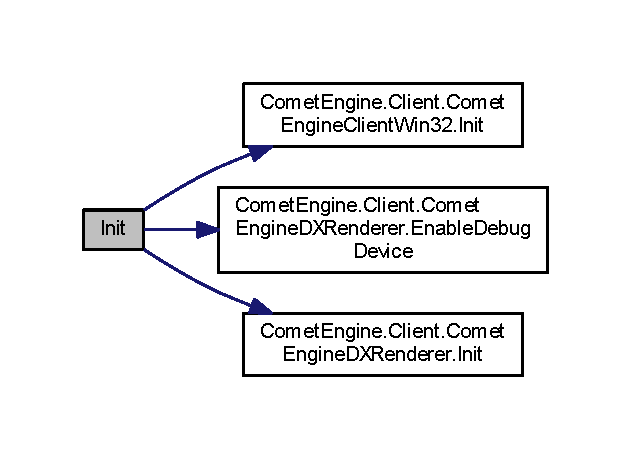
\includegraphics[width=303pt]{class_comet_engine_1_1_client_1_1_comet_engine_client_af5f8db49a5de5bb41cf935066d21f5aa_cgraph}
\end{center}
\end{figure}
이 함수를 호출하는 함수들에 대한 그래프입니다.\+:\nopagebreak
\begin{figure}[H]
\begin{center}
\leavevmode
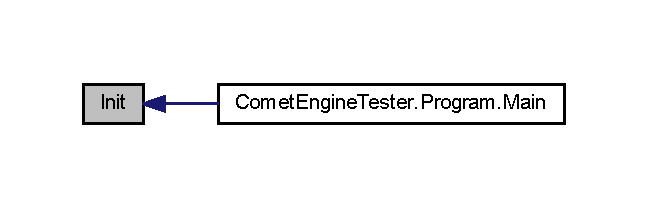
\includegraphics[width=311pt]{class_comet_engine_1_1_client_1_1_comet_engine_client_af5f8db49a5de5bb41cf935066d21f5aa_icgraph}
\end{center}
\end{figure}
\mbox{\Hypertarget{class_comet_engine_1_1_client_1_1_comet_engine_client_aee7b13887a71ba1fcd42c5fbccf124d4}\label{class_comet_engine_1_1_client_1_1_comet_engine_client_aee7b13887a71ba1fcd42c5fbccf124d4}} 
\index{Comet\+Engine\+::\+Client\+::\+Comet\+Engine\+Client@{Comet\+Engine\+::\+Client\+::\+Comet\+Engine\+Client}!Launch@{Launch}}
\index{Launch@{Launch}!Comet\+Engine\+::\+Client\+::\+Comet\+Engine\+Client@{Comet\+Engine\+::\+Client\+::\+Comet\+Engine\+Client}}
\subsubsection{\texorpdfstring{Launch()}{Launch()}}
{\footnotesize\ttfamily static void Launch (\begin{DoxyParamCaption}{ }\end{DoxyParamCaption})\hspace{0.3cm}{\ttfamily [inline]}, {\ttfamily [static]}}



Comet\+Engine\+Client.\+cs 파일의 29 번째 라인에서 정의되었습니다.


\begin{DoxyCode}
30         \{
31             CometEngineClientWin32.Launch();
32         \}
\end{DoxyCode}
이 함수 내부에서 호출하는 함수들에 대한 그래프입니다.\+:\nopagebreak
\begin{figure}[H]
\begin{center}
\leavevmode
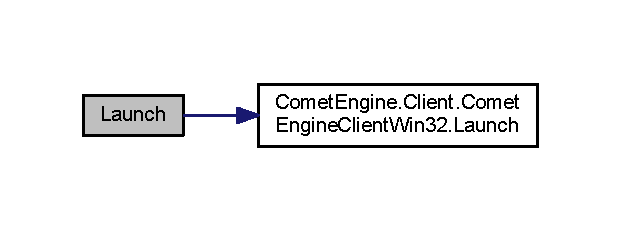
\includegraphics[width=298pt]{class_comet_engine_1_1_client_1_1_comet_engine_client_aee7b13887a71ba1fcd42c5fbccf124d4_cgraph}
\end{center}
\end{figure}
이 함수를 호출하는 함수들에 대한 그래프입니다.\+:\nopagebreak
\begin{figure}[H]
\begin{center}
\leavevmode
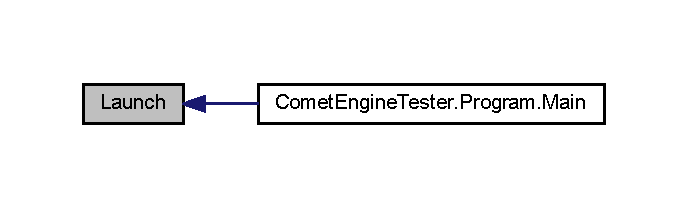
\includegraphics[width=330pt]{class_comet_engine_1_1_client_1_1_comet_engine_client_aee7b13887a71ba1fcd42c5fbccf124d4_icgraph}
\end{center}
\end{figure}


이 클래스에 대한 문서화 페이지는 다음의 파일로부터 생성되었습니다.\+:\begin{DoxyCompactItemize}
\item 
Comet\+Engine\+Client/\+I\+Comet\+Engine\+Client/\hyperlink{_comet_engine_client_8cs}{Comet\+Engine\+Client.\+cs}\end{DoxyCompactItemize}

\hypertarget{class_comet_engine_1_1_client_1_1_comet_engine_client_win32}{}\section{Comet\+Engine\+Client\+Win32 클래스 참조}
\label{class_comet_engine_1_1_client_1_1_comet_engine_client_win32}\index{Comet\+Engine\+Client\+Win32@{Comet\+Engine\+Client\+Win32}}


Comet\+Engine\+Client\+Win32에 대한 협력 다이어그램\+:\nopagebreak
\begin{figure}[H]
\begin{center}
\leavevmode
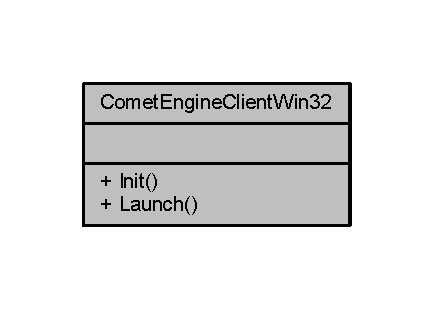
\includegraphics[width=208pt]{class_comet_engine_1_1_client_1_1_comet_engine_client_win32__coll__graph}
\end{center}
\end{figure}
\subsection*{Public 멤버 함수}
\begin{DoxyCompactItemize}
\item 
static bool \hyperlink{class_comet_engine_1_1_client_1_1_comet_engine_client_win32_abc8d29bb16fdbea97c69b9cb6164e3df}{Init} (string Title\+Name, int width, int height, \hyperlink{namespace_comet_engine_1_1_client_a608d2e459fd95babca189e50f4182a65}{W\+Indow\+Modes} mode, Int\+Ptr \hyperlink{_d_l_l_comet_engine_win32_8cpp_a5fb685beb2aed3ecdbad03b352111398}{h\+Instance}, string \hyperlink{_d_l_l_comet_engine_win32_8cpp_af1ff5ad877f6069d41720b03c7769227}{lp\+Cmd\+Line})
\item 
static void \hyperlink{class_comet_engine_1_1_client_1_1_comet_engine_client_win32_aee7b13887a71ba1fcd42c5fbccf124d4}{Launch} ()
\end{DoxyCompactItemize}


\subsection{상세한 설명}


Comet\+Engine\+Client\+Win32.\+cs 파일의 10 번째 라인에서 정의되었습니다.



\subsection{멤버 함수 문서화}
\mbox{\Hypertarget{class_comet_engine_1_1_client_1_1_comet_engine_client_win32_abc8d29bb16fdbea97c69b9cb6164e3df}\label{class_comet_engine_1_1_client_1_1_comet_engine_client_win32_abc8d29bb16fdbea97c69b9cb6164e3df}} 
\index{Comet\+Engine\+::\+Client\+::\+Comet\+Engine\+Client\+Win32@{Comet\+Engine\+::\+Client\+::\+Comet\+Engine\+Client\+Win32}!Init@{Init}}
\index{Init@{Init}!Comet\+Engine\+::\+Client\+::\+Comet\+Engine\+Client\+Win32@{Comet\+Engine\+::\+Client\+::\+Comet\+Engine\+Client\+Win32}}
\subsubsection{\texorpdfstring{Init()}{Init()}}
{\footnotesize\ttfamily static bool Init (\begin{DoxyParamCaption}\item[{string}]{Title\+Name,  }\item[{int}]{width,  }\item[{int}]{height,  }\item[{\hyperlink{namespace_comet_engine_1_1_client_a608d2e459fd95babca189e50f4182a65}{W\+Indow\+Modes}}]{mode,  }\item[{Int\+Ptr}]{h\+Instance,  }\item[{string}]{lp\+Cmd\+Line }\end{DoxyParamCaption})}

이 함수를 호출하는 함수들에 대한 그래프입니다.\+:\nopagebreak
\begin{figure}[H]
\begin{center}
\leavevmode
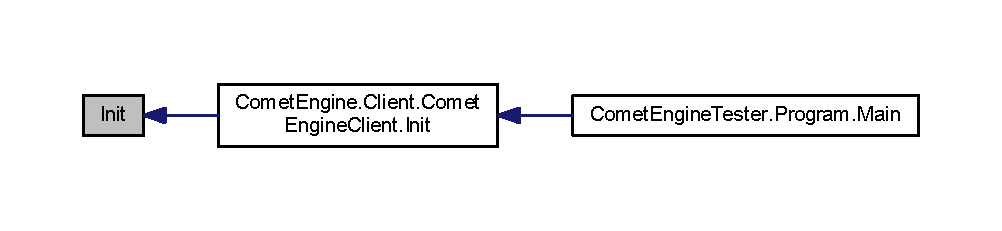
\includegraphics[width=350pt]{class_comet_engine_1_1_client_1_1_comet_engine_client_win32_abc8d29bb16fdbea97c69b9cb6164e3df_icgraph}
\end{center}
\end{figure}
\mbox{\Hypertarget{class_comet_engine_1_1_client_1_1_comet_engine_client_win32_aee7b13887a71ba1fcd42c5fbccf124d4}\label{class_comet_engine_1_1_client_1_1_comet_engine_client_win32_aee7b13887a71ba1fcd42c5fbccf124d4}} 
\index{Comet\+Engine\+::\+Client\+::\+Comet\+Engine\+Client\+Win32@{Comet\+Engine\+::\+Client\+::\+Comet\+Engine\+Client\+Win32}!Launch@{Launch}}
\index{Launch@{Launch}!Comet\+Engine\+::\+Client\+::\+Comet\+Engine\+Client\+Win32@{Comet\+Engine\+::\+Client\+::\+Comet\+Engine\+Client\+Win32}}
\subsubsection{\texorpdfstring{Launch()}{Launch()}}
{\footnotesize\ttfamily static void Launch (\begin{DoxyParamCaption}{ }\end{DoxyParamCaption})}

이 함수를 호출하는 함수들에 대한 그래프입니다.\+:\nopagebreak
\begin{figure}[H]
\begin{center}
\leavevmode
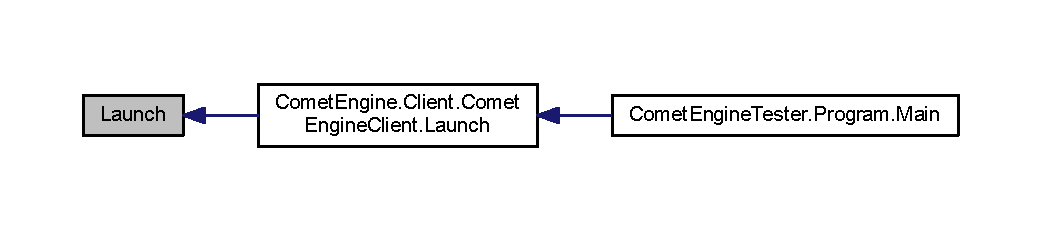
\includegraphics[width=350pt]{class_comet_engine_1_1_client_1_1_comet_engine_client_win32_aee7b13887a71ba1fcd42c5fbccf124d4_icgraph}
\end{center}
\end{figure}


이 클래스에 대한 문서화 페이지는 다음의 파일로부터 생성되었습니다.\+:\begin{DoxyCompactItemize}
\item 
Comet\+Engine\+Client/\+I\+Comet\+Engine\+Client/\hyperlink{_comet_engine_client_win32_8cs}{Comet\+Engine\+Client\+Win32.\+cs}\end{DoxyCompactItemize}

\hypertarget{class_comet_engine_1_1_client_1_1_comet_engine_d_x_renderer}{}\section{Comet\+Engine\+D\+X\+Renderer 클래스 참조}
\label{class_comet_engine_1_1_client_1_1_comet_engine_d_x_renderer}\index{Comet\+Engine\+D\+X\+Renderer@{Comet\+Engine\+D\+X\+Renderer}}


Comet\+Engine\+D\+X\+Renderer에 대한 협력 다이어그램\+:\nopagebreak
\begin{figure}[H]
\begin{center}
\leavevmode
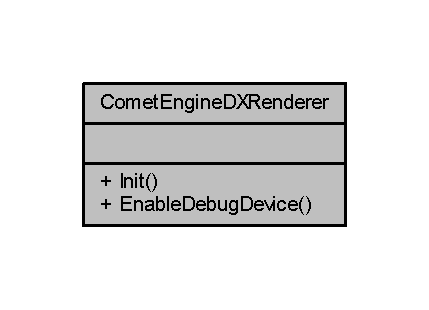
\includegraphics[width=206pt]{class_comet_engine_1_1_client_1_1_comet_engine_d_x_renderer__coll__graph}
\end{center}
\end{figure}
\subsection*{Public 멤버 함수}
\begin{DoxyCompactItemize}
\item 
static bool \hyperlink{class_comet_engine_1_1_client_1_1_comet_engine_d_x_renderer_a43593e265ce79b6ab88f4384039eacc7}{Init} (int i\+\_\+\+Render\+Width, int \hyperlink{_d_l_l_comet_engine_renderer_8cpp_ab996e2b2e12adfc087c67cebde9194e6}{i\+\_\+\+Render\+Height}, int \hyperlink{_d_l_l_comet_engine_renderer_8cpp_a901222d6138bd4efc54d4eda8460c65b}{i\+\_\+\+Render\+Scale}, int \hyperlink{_d_l_l_comet_engine_renderer_8cpp_a7016fffcce13da83a94427468f9bf950}{i\+\_\+\+M\+S\+A\+A\+Scale}, bool Is\+Full\+Screen)
\begin{DoxyCompactList}\small\item\em Initalize for Comet\+Engin Direct\+X11 \hyperlink{namespace_comet_engine_1_1_renderer}{Renderer} \end{DoxyCompactList}\item 
static void \hyperlink{class_comet_engine_1_1_client_1_1_comet_engine_d_x_renderer_a8385160d1bc564a68d4211dda3015d46}{Enable\+Debug\+Device} (bool i\+\_\+\+Flag)
\begin{DoxyCompactList}\small\item\em Direct\+X11 Debug Device Enable \end{DoxyCompactList}\end{DoxyCompactItemize}


\subsection{상세한 설명}


Comet\+Engine\+D\+X\+Renderer.\+cs 파일의 10 번째 라인에서 정의되었습니다.



\subsection{멤버 함수 문서화}
\mbox{\Hypertarget{class_comet_engine_1_1_client_1_1_comet_engine_d_x_renderer_a8385160d1bc564a68d4211dda3015d46}\label{class_comet_engine_1_1_client_1_1_comet_engine_d_x_renderer_a8385160d1bc564a68d4211dda3015d46}} 
\index{Comet\+Engine\+::\+Client\+::\+Comet\+Engine\+D\+X\+Renderer@{Comet\+Engine\+::\+Client\+::\+Comet\+Engine\+D\+X\+Renderer}!Enable\+Debug\+Device@{Enable\+Debug\+Device}}
\index{Enable\+Debug\+Device@{Enable\+Debug\+Device}!Comet\+Engine\+::\+Client\+::\+Comet\+Engine\+D\+X\+Renderer@{Comet\+Engine\+::\+Client\+::\+Comet\+Engine\+D\+X\+Renderer}}
\subsubsection{\texorpdfstring{Enable\+Debug\+Device()}{EnableDebugDevice()}}
{\footnotesize\ttfamily static void Enable\+Debug\+Device (\begin{DoxyParamCaption}\item[{bool}]{i\+\_\+\+Flag }\end{DoxyParamCaption})}



Direct\+X11 Debug Device Enable 


\begin{DoxyParams}{매개변수}
{\em i\+\_\+\+Flag} & \\
\hline
\end{DoxyParams}
이 함수를 호출하는 함수들에 대한 그래프입니다.\+:\nopagebreak
\begin{figure}[H]
\begin{center}
\leavevmode
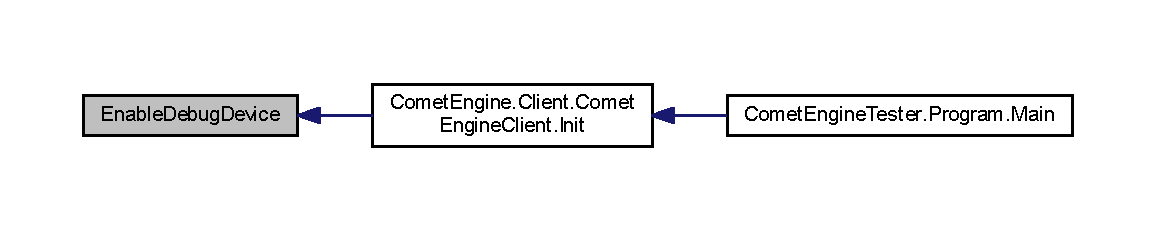
\includegraphics[width=350pt]{class_comet_engine_1_1_client_1_1_comet_engine_d_x_renderer_a8385160d1bc564a68d4211dda3015d46_icgraph}
\end{center}
\end{figure}
\mbox{\Hypertarget{class_comet_engine_1_1_client_1_1_comet_engine_d_x_renderer_a43593e265ce79b6ab88f4384039eacc7}\label{class_comet_engine_1_1_client_1_1_comet_engine_d_x_renderer_a43593e265ce79b6ab88f4384039eacc7}} 
\index{Comet\+Engine\+::\+Client\+::\+Comet\+Engine\+D\+X\+Renderer@{Comet\+Engine\+::\+Client\+::\+Comet\+Engine\+D\+X\+Renderer}!Init@{Init}}
\index{Init@{Init}!Comet\+Engine\+::\+Client\+::\+Comet\+Engine\+D\+X\+Renderer@{Comet\+Engine\+::\+Client\+::\+Comet\+Engine\+D\+X\+Renderer}}
\subsubsection{\texorpdfstring{Init()}{Init()}}
{\footnotesize\ttfamily static bool Init (\begin{DoxyParamCaption}\item[{int}]{i\+\_\+\+Render\+Width,  }\item[{int}]{i\+\_\+\+Render\+Height,  }\item[{int}]{i\+\_\+\+Render\+Scale,  }\item[{int}]{i\+\_\+\+M\+S\+A\+A\+Scale,  }\item[{bool}]{Is\+Full\+Screen }\end{DoxyParamCaption})}



Initalize for Comet\+Engin Direct\+X11 \hyperlink{namespace_comet_engine_1_1_renderer}{Renderer} 


\begin{DoxyParams}{매개변수}
{\em i\+\_\+\+Render\+Width} & Rendering Width\\
\hline
{\em i\+\_\+\+Render\+Height} & Rendering Height\\
\hline
{\em i\+\_\+\+Render\+Scale} & Rendering Scale\\
\hline
{\em i\+\_\+\+M\+S\+A\+A\+Scale} & M\+S\+AA Scale less 1 is No M\+S\+AA\\
\hline
{\em Is\+Full\+Screen} & DirectX Full\+Screen Flag\\
\hline
\end{DoxyParams}
\begin{DoxyReturn}{반환값}

\end{DoxyReturn}
이 함수를 호출하는 함수들에 대한 그래프입니다.\+:\nopagebreak
\begin{figure}[H]
\begin{center}
\leavevmode
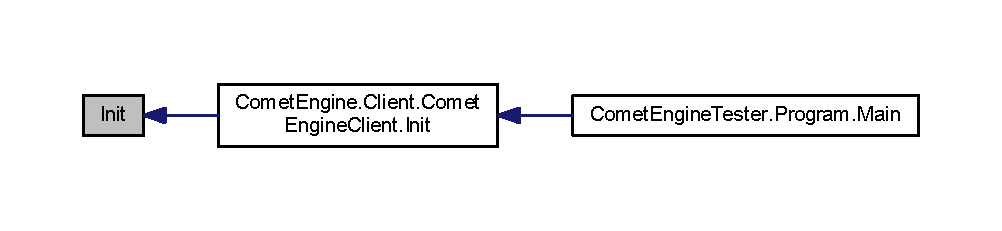
\includegraphics[width=350pt]{class_comet_engine_1_1_client_1_1_comet_engine_d_x_renderer_a43593e265ce79b6ab88f4384039eacc7_icgraph}
\end{center}
\end{figure}


이 클래스에 대한 문서화 페이지는 다음의 파일로부터 생성되었습니다.\+:\begin{DoxyCompactItemize}
\item 
Comet\+Engine\+Client/\+I\+Comet\+Engine\+Client/\hyperlink{_comet_engine_d_x_renderer_8cs}{Comet\+Engine\+D\+X\+Renderer.\+cs}\end{DoxyCompactItemize}

\hypertarget{class_comet_engine_1_1_renderer_1_1_comet_engine_d_x_renderer}{}\section{Comet\+Engine\+D\+X\+Renderer 클래스 참조}
\label{class_comet_engine_1_1_renderer_1_1_comet_engine_d_x_renderer}\index{Comet\+Engine\+D\+X\+Renderer@{Comet\+Engine\+D\+X\+Renderer}}


{\ttfamily \#include $<$Comet\+Engine\+D\+X\+Renderer.\+h$>$}



Comet\+Engine\+D\+X\+Renderer에 대한 협력 다이어그램\+:\nopagebreak
\begin{figure}[H]
\begin{center}
\leavevmode
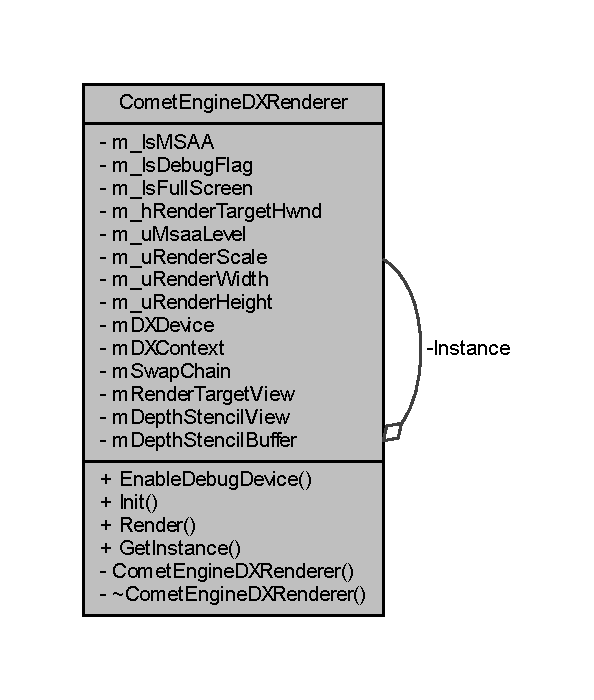
\includegraphics[width=285pt]{class_comet_engine_1_1_renderer_1_1_comet_engine_d_x_renderer__coll__graph}
\end{center}
\end{figure}
\subsection*{Public 멤버 함수}
\begin{DoxyCompactItemize}
\item 
void \hyperlink{class_comet_engine_1_1_renderer_1_1_comet_engine_d_x_renderer_a0cec813dd654a43d162981c37b0cbf6e}{Enable\+Debug\+Device} (bool i\+\_\+\+Flag)
\item 
bool \hyperlink{class_comet_engine_1_1_renderer_1_1_comet_engine_d_x_renderer_a570783c0a51edd5394fdb16137ae37c1}{Init} (int i\+\_\+\+Render\+Width, int \hyperlink{_d_l_l_comet_engine_renderer_8cpp_ab996e2b2e12adfc087c67cebde9194e6}{i\+\_\+\+Render\+Height}, int \hyperlink{_d_l_l_comet_engine_renderer_8cpp_a901222d6138bd4efc54d4eda8460c65b}{i\+\_\+\+Render\+Scale}, int \hyperlink{_d_l_l_comet_engine_renderer_8cpp_a7016fffcce13da83a94427468f9bf950}{i\+\_\+\+M\+S\+A\+A\+Scale}, bool is\+Full\+Screen)
\item 
void \hyperlink{class_comet_engine_1_1_renderer_1_1_comet_engine_d_x_renderer_ac6fa4f62b984d0d34e785bd960255d71}{Render} (float dt)
\end{DoxyCompactItemize}
\subsection*{정적 Public 멤버 함수}
\begin{DoxyCompactItemize}
\item 
static \hyperlink{class_comet_engine_1_1_renderer_1_1_comet_engine_d_x_renderer}{Comet\+Engine\+D\+X\+Renderer} $\ast$ \hyperlink{class_comet_engine_1_1_renderer_1_1_comet_engine_d_x_renderer_a9894517531990b824a58e1f61c6d542e}{Get\+Instance} ()
\end{DoxyCompactItemize}
\subsection*{Private 멤버 함수}
\begin{DoxyCompactItemize}
\item 
\hyperlink{class_comet_engine_1_1_renderer_1_1_comet_engine_d_x_renderer_a5d4d4453042540bd1f4e4a36229b62f6}{Comet\+Engine\+D\+X\+Renderer} ()
\item 
\hyperlink{class_comet_engine_1_1_renderer_1_1_comet_engine_d_x_renderer_a7ec2ab41325dc127a1780c88d84a81e2}{$\sim$\+Comet\+Engine\+D\+X\+Renderer} ()
\end{DoxyCompactItemize}
\subsection*{Private 속성}
\begin{DoxyCompactItemize}
\item 
B\+O\+OL \hyperlink{class_comet_engine_1_1_renderer_1_1_comet_engine_d_x_renderer_ade12531fe5dd3f80e38d0baf16fe2c3f}{m\+\_\+\+Is\+M\+S\+AA}
\item 
B\+O\+OL \hyperlink{class_comet_engine_1_1_renderer_1_1_comet_engine_d_x_renderer_a4605315a46596f062351adb5071a334c}{m\+\_\+\+Is\+Debug\+Flag}
\item 
B\+O\+OL \hyperlink{class_comet_engine_1_1_renderer_1_1_comet_engine_d_x_renderer_aa6179af78a783f7c0d77d6ea9b95abfb}{m\+\_\+\+Is\+Full\+Screen}
\item 
H\+W\+ND \hyperlink{class_comet_engine_1_1_renderer_1_1_comet_engine_d_x_renderer_a6ec5b124115c13d09e631e3245ba0264}{m\+\_\+h\+Render\+Target\+Hwnd}
\item 
U\+I\+NT \hyperlink{class_comet_engine_1_1_renderer_1_1_comet_engine_d_x_renderer_aee26a00f9adfbcf0a5de3a91ec7e322d}{m\+\_\+u\+Msaa\+Level}
\item 
U\+I\+NT \hyperlink{class_comet_engine_1_1_renderer_1_1_comet_engine_d_x_renderer_a00acfc4bfe2d732584f5ae0cb28186d8}{m\+\_\+u\+Render\+Scale}
\item 
U\+I\+NT \hyperlink{class_comet_engine_1_1_renderer_1_1_comet_engine_d_x_renderer_a3127a8dc19e4bd799fa7e1bfff28de11}{m\+\_\+u\+Render\+Width}
\item 
U\+I\+NT \hyperlink{class_comet_engine_1_1_renderer_1_1_comet_engine_d_x_renderer_af8f780a50f9325d3bad66c1ba49ed533}{m\+\_\+u\+Render\+Height}
\item 
I\+D3\+D11\+Device $\ast$ \hyperlink{class_comet_engine_1_1_renderer_1_1_comet_engine_d_x_renderer_ac606b85554250d2e65a2aa9f10e6aa45}{m\+D\+X\+Device}
\item 
I\+D3\+D11\+Device\+Context $\ast$ \hyperlink{class_comet_engine_1_1_renderer_1_1_comet_engine_d_x_renderer_ad38b8ad7fd1c747698a96256e75eb635}{m\+D\+X\+Context}
\item 
I\+D\+X\+G\+I\+Swap\+Chain $\ast$ \hyperlink{class_comet_engine_1_1_renderer_1_1_comet_engine_d_x_renderer_a501ef6e0fe112727e82e727997af01c6}{m\+Swap\+Chain}
\item 
I\+D3\+D11\+Render\+Target\+View $\ast$ \hyperlink{class_comet_engine_1_1_renderer_1_1_comet_engine_d_x_renderer_a109e138c97280440a0955d475441f49d}{m\+Render\+Target\+View}
\item 
I\+D3\+D11\+Depth\+Stencil\+View $\ast$ \hyperlink{class_comet_engine_1_1_renderer_1_1_comet_engine_d_x_renderer_a01cc1c2c77d9af90d45c250d51bcfa35}{m\+Depth\+Stencil\+View}
\item 
I\+D3\+D11\+Texture2D $\ast$ \hyperlink{class_comet_engine_1_1_renderer_1_1_comet_engine_d_x_renderer_a738b786f64e4fc6c9a2355f1cf9ae830}{m\+Depth\+Stencil\+Buffer}
\end{DoxyCompactItemize}
\subsection*{정적 Private 속성}
\begin{DoxyCompactItemize}
\item 
static \hyperlink{class_comet_engine_1_1_renderer_1_1_comet_engine_d_x_renderer}{Comet\+Engine\+D\+X\+Renderer} $\ast$ \hyperlink{class_comet_engine_1_1_renderer_1_1_comet_engine_d_x_renderer_af2bbff1b1d0120cc652b4f2198ddb04a}{Instance} = nullptr
\end{DoxyCompactItemize}


\subsection{상세한 설명}


Comet\+Engine\+D\+X\+Renderer.\+h 파일의 14 번째 라인에서 정의되었습니다.



\subsection{생성자 \& 소멸자 문서화}
\mbox{\Hypertarget{class_comet_engine_1_1_renderer_1_1_comet_engine_d_x_renderer_a5d4d4453042540bd1f4e4a36229b62f6}\label{class_comet_engine_1_1_renderer_1_1_comet_engine_d_x_renderer_a5d4d4453042540bd1f4e4a36229b62f6}} 
\index{Comet\+Engine\+::\+Renderer\+::\+Comet\+Engine\+D\+X\+Renderer@{Comet\+Engine\+::\+Renderer\+::\+Comet\+Engine\+D\+X\+Renderer}!Comet\+Engine\+D\+X\+Renderer@{Comet\+Engine\+D\+X\+Renderer}}
\index{Comet\+Engine\+D\+X\+Renderer@{Comet\+Engine\+D\+X\+Renderer}!Comet\+Engine\+::\+Renderer\+::\+Comet\+Engine\+D\+X\+Renderer@{Comet\+Engine\+::\+Renderer\+::\+Comet\+Engine\+D\+X\+Renderer}}
\subsubsection{\texorpdfstring{Comet\+Engine\+D\+X\+Renderer()}{CometEngineDXRenderer()}}
{\footnotesize\ttfamily \hyperlink{class_comet_engine_1_1_renderer_1_1_comet_engine_d_x_renderer}{Comet\+Engine\+D\+X\+Renderer} (\begin{DoxyParamCaption}{ }\end{DoxyParamCaption})\hspace{0.3cm}{\ttfamily [inline]}, {\ttfamily [private]}}



Comet\+Engine\+D\+X\+Renderer.\+h 파일의 26 번째 라인에서 정의되었습니다.


\begin{DoxyCode}
26 \{\}
\end{DoxyCode}
이 함수 내부에서 호출하는 함수들에 대한 그래프입니다.\+:\nopagebreak
\begin{figure}[H]
\begin{center}
\leavevmode
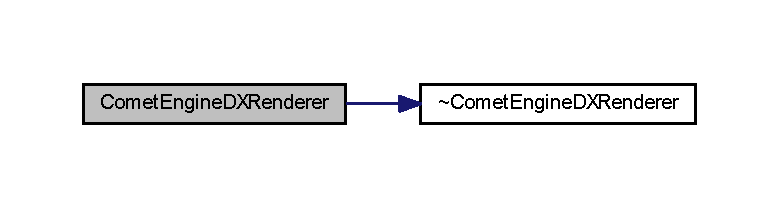
\includegraphics[width=350pt]{class_comet_engine_1_1_renderer_1_1_comet_engine_d_x_renderer_a5d4d4453042540bd1f4e4a36229b62f6_cgraph}
\end{center}
\end{figure}
이 함수를 호출하는 함수들에 대한 그래프입니다.\+:\nopagebreak
\begin{figure}[H]
\begin{center}
\leavevmode
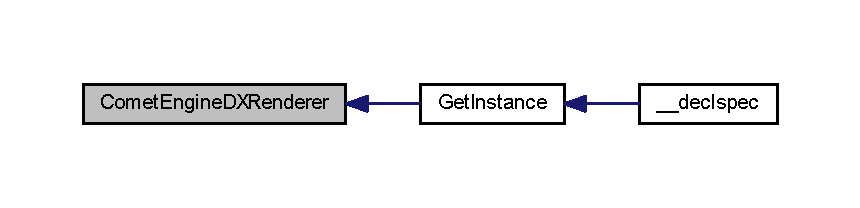
\includegraphics[width=350pt]{class_comet_engine_1_1_renderer_1_1_comet_engine_d_x_renderer_a5d4d4453042540bd1f4e4a36229b62f6_icgraph}
\end{center}
\end{figure}
\mbox{\Hypertarget{class_comet_engine_1_1_renderer_1_1_comet_engine_d_x_renderer_a7ec2ab41325dc127a1780c88d84a81e2}\label{class_comet_engine_1_1_renderer_1_1_comet_engine_d_x_renderer_a7ec2ab41325dc127a1780c88d84a81e2}} 
\index{Comet\+Engine\+::\+Renderer\+::\+Comet\+Engine\+D\+X\+Renderer@{Comet\+Engine\+::\+Renderer\+::\+Comet\+Engine\+D\+X\+Renderer}!````~Comet\+Engine\+D\+X\+Renderer@{$\sim$\+Comet\+Engine\+D\+X\+Renderer}}
\index{````~Comet\+Engine\+D\+X\+Renderer@{$\sim$\+Comet\+Engine\+D\+X\+Renderer}!Comet\+Engine\+::\+Renderer\+::\+Comet\+Engine\+D\+X\+Renderer@{Comet\+Engine\+::\+Renderer\+::\+Comet\+Engine\+D\+X\+Renderer}}
\subsubsection{\texorpdfstring{$\sim$\+Comet\+Engine\+D\+X\+Renderer()}{~CometEngineDXRenderer()}}
{\footnotesize\ttfamily $\sim$\hyperlink{class_comet_engine_1_1_renderer_1_1_comet_engine_d_x_renderer}{Comet\+Engine\+D\+X\+Renderer} (\begin{DoxyParamCaption}{ }\end{DoxyParamCaption})\hspace{0.3cm}{\ttfamily [private]}}



Comet\+Engine\+D\+X\+Renderer.\+cpp 파일의 138 번째 라인에서 정의되었습니다.


\begin{DoxyCode}
139 \{
140     \hyperlink{class_comet_engine_1_1_renderer_1_1_comet_engine_d_x_renderer_a501ef6e0fe112727e82e727997af01c6}{mSwapChain}->Release();
141     \hyperlink{class_comet_engine_1_1_renderer_1_1_comet_engine_d_x_renderer_a01cc1c2c77d9af90d45c250d51bcfa35}{mDepthStencilView}->Release();
142     \hyperlink{class_comet_engine_1_1_renderer_1_1_comet_engine_d_x_renderer_ac606b85554250d2e65a2aa9f10e6aa45}{mDXDevice}->Release();
143     \hyperlink{class_comet_engine_1_1_renderer_1_1_comet_engine_d_x_renderer_ad38b8ad7fd1c747698a96256e75eb635}{mDXContext}->Release();
144     \hyperlink{class_comet_engine_1_1_renderer_1_1_comet_engine_d_x_renderer_a109e138c97280440a0955d475441f49d}{mRenderTargetView}->Release();
145     \hyperlink{class_comet_engine_1_1_renderer_1_1_comet_engine_d_x_renderer_a738b786f64e4fc6c9a2355f1cf9ae830}{mDepthStencilBuffer}->Release();
146 \}
\end{DoxyCode}
이 함수를 호출하는 함수들에 대한 그래프입니다.\+:\nopagebreak
\begin{figure}[H]
\begin{center}
\leavevmode
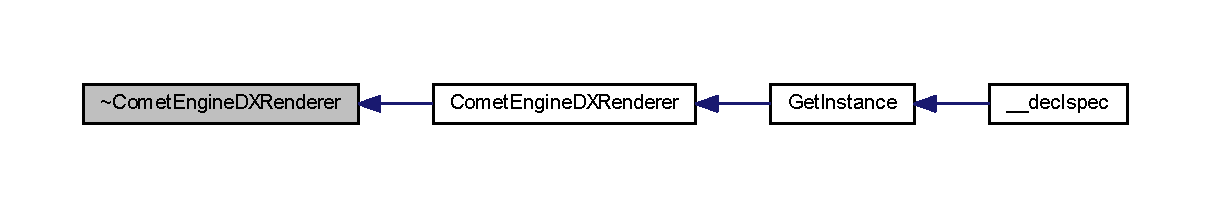
\includegraphics[width=350pt]{class_comet_engine_1_1_renderer_1_1_comet_engine_d_x_renderer_a7ec2ab41325dc127a1780c88d84a81e2_icgraph}
\end{center}
\end{figure}


\subsection{멤버 함수 문서화}
\mbox{\Hypertarget{class_comet_engine_1_1_renderer_1_1_comet_engine_d_x_renderer_a0cec813dd654a43d162981c37b0cbf6e}\label{class_comet_engine_1_1_renderer_1_1_comet_engine_d_x_renderer_a0cec813dd654a43d162981c37b0cbf6e}} 
\index{Comet\+Engine\+::\+Renderer\+::\+Comet\+Engine\+D\+X\+Renderer@{Comet\+Engine\+::\+Renderer\+::\+Comet\+Engine\+D\+X\+Renderer}!Enable\+Debug\+Device@{Enable\+Debug\+Device}}
\index{Enable\+Debug\+Device@{Enable\+Debug\+Device}!Comet\+Engine\+::\+Renderer\+::\+Comet\+Engine\+D\+X\+Renderer@{Comet\+Engine\+::\+Renderer\+::\+Comet\+Engine\+D\+X\+Renderer}}
\subsubsection{\texorpdfstring{Enable\+Debug\+Device()}{EnableDebugDevice()}}
{\footnotesize\ttfamily void Enable\+Debug\+Device (\begin{DoxyParamCaption}\item[{bool}]{i\+\_\+\+Flag }\end{DoxyParamCaption})}



Comet\+Engine\+D\+X\+Renderer.\+cpp 파일의 19 번째 라인에서 정의되었습니다.


\begin{DoxyCode}
20 \{
21     \hyperlink{class_comet_engine_1_1_renderer_1_1_comet_engine_d_x_renderer_a4605315a46596f062351adb5071a334c}{m\_IsDebugFlag} = i\_Flag;
22 \}
\end{DoxyCode}
이 함수를 호출하는 함수들에 대한 그래프입니다.\+:\nopagebreak
\begin{figure}[H]
\begin{center}
\leavevmode
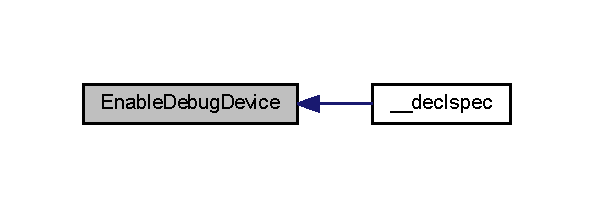
\includegraphics[width=285pt]{class_comet_engine_1_1_renderer_1_1_comet_engine_d_x_renderer_a0cec813dd654a43d162981c37b0cbf6e_icgraph}
\end{center}
\end{figure}
\mbox{\Hypertarget{class_comet_engine_1_1_renderer_1_1_comet_engine_d_x_renderer_a9894517531990b824a58e1f61c6d542e}\label{class_comet_engine_1_1_renderer_1_1_comet_engine_d_x_renderer_a9894517531990b824a58e1f61c6d542e}} 
\index{Comet\+Engine\+::\+Renderer\+::\+Comet\+Engine\+D\+X\+Renderer@{Comet\+Engine\+::\+Renderer\+::\+Comet\+Engine\+D\+X\+Renderer}!Get\+Instance@{Get\+Instance}}
\index{Get\+Instance@{Get\+Instance}!Comet\+Engine\+::\+Renderer\+::\+Comet\+Engine\+D\+X\+Renderer@{Comet\+Engine\+::\+Renderer\+::\+Comet\+Engine\+D\+X\+Renderer}}
\subsubsection{\texorpdfstring{Get\+Instance()}{GetInstance()}}
{\footnotesize\ttfamily \hyperlink{class_comet_engine_1_1_renderer_1_1_comet_engine_d_x_renderer}{Comet\+Engine\+D\+X\+Renderer} $\ast$ Get\+Instance (\begin{DoxyParamCaption}{ }\end{DoxyParamCaption})\hspace{0.3cm}{\ttfamily [static]}}



Comet\+Engine\+D\+X\+Renderer.\+cpp 파일의 11 번째 라인에서 정의되었습니다.


\begin{DoxyCode}
12 \{
13     \textcolor{keywordflow}{if} (\hyperlink{class_comet_engine_1_1_renderer_1_1_comet_engine_d_x_renderer_af2bbff1b1d0120cc652b4f2198ddb04a}{Instance} == \textcolor{keyword}{nullptr})
14         \hyperlink{class_comet_engine_1_1_renderer_1_1_comet_engine_d_x_renderer_af2bbff1b1d0120cc652b4f2198ddb04a}{Instance} = \textcolor{keyword}{new} \hyperlink{class_comet_engine_1_1_renderer_1_1_comet_engine_d_x_renderer_a5d4d4453042540bd1f4e4a36229b62f6}{CometEngineDXRenderer}();
15     \textcolor{keywordflow}{return} \hyperlink{class_comet_engine_1_1_renderer_1_1_comet_engine_d_x_renderer_af2bbff1b1d0120cc652b4f2198ddb04a}{Instance};
16 
17 \}
\end{DoxyCode}
이 함수 내부에서 호출하는 함수들에 대한 그래프입니다.\+:\nopagebreak
\begin{figure}[H]
\begin{center}
\leavevmode
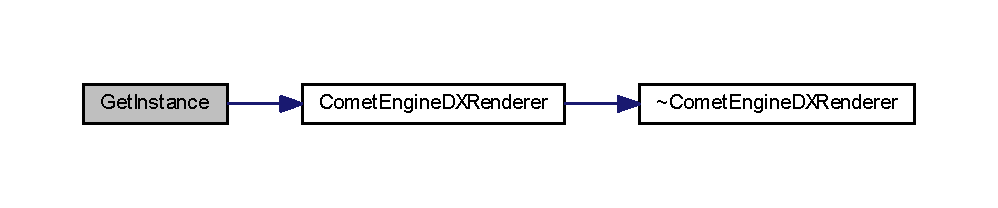
\includegraphics[width=350pt]{class_comet_engine_1_1_renderer_1_1_comet_engine_d_x_renderer_a9894517531990b824a58e1f61c6d542e_cgraph}
\end{center}
\end{figure}
이 함수를 호출하는 함수들에 대한 그래프입니다.\+:\nopagebreak
\begin{figure}[H]
\begin{center}
\leavevmode
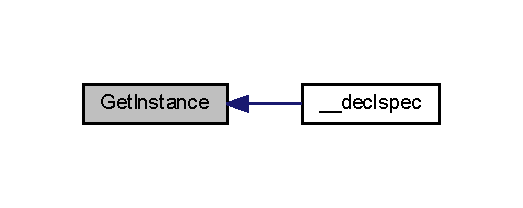
\includegraphics[width=251pt]{class_comet_engine_1_1_renderer_1_1_comet_engine_d_x_renderer_a9894517531990b824a58e1f61c6d542e_icgraph}
\end{center}
\end{figure}
\mbox{\Hypertarget{class_comet_engine_1_1_renderer_1_1_comet_engine_d_x_renderer_a570783c0a51edd5394fdb16137ae37c1}\label{class_comet_engine_1_1_renderer_1_1_comet_engine_d_x_renderer_a570783c0a51edd5394fdb16137ae37c1}} 
\index{Comet\+Engine\+::\+Renderer\+::\+Comet\+Engine\+D\+X\+Renderer@{Comet\+Engine\+::\+Renderer\+::\+Comet\+Engine\+D\+X\+Renderer}!Init@{Init}}
\index{Init@{Init}!Comet\+Engine\+::\+Renderer\+::\+Comet\+Engine\+D\+X\+Renderer@{Comet\+Engine\+::\+Renderer\+::\+Comet\+Engine\+D\+X\+Renderer}}
\subsubsection{\texorpdfstring{Init()}{Init()}}
{\footnotesize\ttfamily bool Init (\begin{DoxyParamCaption}\item[{int}]{i\+\_\+\+Render\+Width,  }\item[{int}]{i\+\_\+\+Render\+Height,  }\item[{int}]{i\+\_\+\+Render\+Scale,  }\item[{int}]{i\+\_\+\+M\+S\+A\+A\+Scale,  }\item[{bool}]{is\+Full\+Screen }\end{DoxyParamCaption})}



Comet\+Engine\+D\+X\+Renderer.\+cpp 파일의 24 번째 라인에서 정의되었습니다.


\begin{DoxyCode}
25 \{
26     \hyperlink{class_comet_engine_1_1_renderer_1_1_comet_engine_d_x_renderer_a3127a8dc19e4bd799fa7e1bfff28de11}{m\_uRenderWidth}  = i\_RenderWidth;
27     \hyperlink{class_comet_engine_1_1_renderer_1_1_comet_engine_d_x_renderer_af8f780a50f9325d3bad66c1ba49ed533}{m\_uRenderHeight} = \hyperlink{_d_l_l_comet_engine_renderer_8cpp_ab996e2b2e12adfc087c67cebde9194e6}{i\_RenderHeight};
28     \hyperlink{class_comet_engine_1_1_renderer_1_1_comet_engine_d_x_renderer_a00acfc4bfe2d732584f5ae0cb28186d8}{m\_uRenderScale} = \hyperlink{_d_l_l_comet_engine_renderer_8cpp_a901222d6138bd4efc54d4eda8460c65b}{i\_RenderScale};
29     \hyperlink{class_comet_engine_1_1_renderer_1_1_comet_engine_d_x_renderer_aee26a00f9adfbcf0a5de3a91ec7e322d}{m\_uMsaaLevel} = \hyperlink{_d_l_l_comet_engine_renderer_8cpp_a7016fffcce13da83a94427468f9bf950}{i\_MSAAScale};
30     \hyperlink{class_comet_engine_1_1_renderer_1_1_comet_engine_d_x_renderer_aa6179af78a783f7c0d77d6ea9b95abfb}{m\_IsFullScreen} = isFullScreen;
31 
32     UINT flags = 0;
33     \textcolor{keywordflow}{if} (\hyperlink{class_comet_engine_1_1_renderer_1_1_comet_engine_d_x_renderer_a4605315a46596f062351adb5071a334c}{m\_IsDebugFlag})
34         flags |= D3D11\_CREATE\_DEVICE\_DEBUG;
35     D3D\_FEATURE\_LEVEL Featurelevel;
36     \hyperlink{_comet_engine_d_x_renderer_8cpp_a924cd8cbf81756869040aed04fd33ca5}{HR}(D3D11CreateDevice(\textcolor{keyword}{nullptr}, D3D\_DRIVER\_TYPE\_HARDWARE, \textcolor{keyword}{nullptr}, flags, 0, 0, D3D11\_SDK\_VERSION, &
      \hyperlink{class_comet_engine_1_1_renderer_1_1_comet_engine_d_x_renderer_ac606b85554250d2e65a2aa9f10e6aa45}{mDXDevice}, &Featurelevel, &\hyperlink{class_comet_engine_1_1_renderer_1_1_comet_engine_d_x_renderer_ad38b8ad7fd1c747698a96256e75eb635}{mDXContext}));
37 
38     DXGI\_SWAP\_CHAIN\_DESC swap\_chain\_desc = \{ 0 \};
39     swap\_chain\_desc.BufferDesc.Width = \hyperlink{class_comet_engine_1_1_renderer_1_1_comet_engine_d_x_renderer_a3127a8dc19e4bd799fa7e1bfff28de11}{m\_uRenderWidth};
40     swap\_chain\_desc.BufferDesc.Height = \hyperlink{class_comet_engine_1_1_renderer_1_1_comet_engine_d_x_renderer_af8f780a50f9325d3bad66c1ba49ed533}{m\_uRenderHeight};
41     swap\_chain\_desc.BufferDesc.RefreshRate.Numerator = 60;
42     swap\_chain\_desc.BufferDesc.RefreshRate.Denominator = 1;
43     swap\_chain\_desc.BufferDesc.Format = DXGI\_FORMAT\_R8G8B8A8\_UNORM;
44     swap\_chain\_desc.BufferDesc.ScanlineOrdering = DXGI\_MODE\_SCANLINE\_ORDER\_UNSPECIFIED;
45     swap\_chain\_desc.BufferDesc.Scaling = DXGI\_MODE\_SCALING\_UNSPECIFIED;
46 
47     UINT MsaaQulity;
48     \hyperlink{_comet_engine_d_x_renderer_8cpp_a924cd8cbf81756869040aed04fd33ca5}{HR}(\hyperlink{class_comet_engine_1_1_renderer_1_1_comet_engine_d_x_renderer_ac606b85554250d2e65a2aa9f10e6aa45}{mDXDevice}->CheckMultisampleQualityLevels(DXGI\_FORMAT\_R8G8B8A8\_UNORM, 
      \hyperlink{class_comet_engine_1_1_renderer_1_1_comet_engine_d_x_renderer_aee26a00f9adfbcf0a5de3a91ec7e322d}{m\_uMsaaLevel}, &MsaaQulity));
49 
50     assert(MsaaQulity > 0);
51     \textcolor{keywordflow}{if} (\hyperlink{class_comet_engine_1_1_renderer_1_1_comet_engine_d_x_renderer_aee26a00f9adfbcf0a5de3a91ec7e322d}{m\_uMsaaLevel} > 1)
52     \{
53         swap\_chain\_desc.SampleDesc.Count = \hyperlink{class_comet_engine_1_1_renderer_1_1_comet_engine_d_x_renderer_aee26a00f9adfbcf0a5de3a91ec7e322d}{m\_uMsaaLevel};
54         swap\_chain\_desc.SampleDesc.Quality = MsaaQulity - 1;
55     \}
56     \textcolor{keywordflow}{else}
57     \{
58         swap\_chain\_desc.SampleDesc.Count = 1;
59         swap\_chain\_desc.SampleDesc.Quality = 0;
60     \}
61     swap\_chain\_desc.BufferUsage = DXGI\_USAGE\_RENDER\_TARGET\_OUTPUT;
62     swap\_chain\_desc.BufferCount = 1;
63     swap\_chain\_desc.OutputWindow = \hyperlink{class_comet_engine_1_1_renderer_1_1_comet_engine_d_x_renderer_a6ec5b124115c13d09e631e3245ba0264}{m\_hRenderTargetHwnd};
64     swap\_chain\_desc.Windowed = \hyperlink{class_comet_engine_1_1_renderer_1_1_comet_engine_d_x_renderer_aa6179af78a783f7c0d77d6ea9b95abfb}{m\_IsFullScreen};
65     swap\_chain\_desc.SwapEffect = DXGI\_SWAP\_EFFECT\_DISCARD;
66     swap\_chain\_desc.Flags = DXGI\_SWAP\_CHAIN\_FLAG\_ALLOW\_MODE\_SWITCH;
67     DXGI\_ADAPTER\_DESC desc;
68 
69     IDXGIDevice*    dxgiDevice = \textcolor{keyword}{nullptr};
70     IDXGIAdapter*   dxgiAdapter = \textcolor{keyword}{nullptr};
71     IDXGIFactory*   dxgiFactory = \textcolor{keyword}{nullptr};
72     ID3D11Texture2D* BackBuffer;
73     \hyperlink{_comet_engine_d_x_renderer_8cpp_a924cd8cbf81756869040aed04fd33ca5}{HR}(\hyperlink{class_comet_engine_1_1_renderer_1_1_comet_engine_d_x_renderer_ac606b85554250d2e65a2aa9f10e6aa45}{mDXDevice}->QueryInterface(\_\_uuidof(IDXGIDevice), (\textcolor{keywordtype}{void}**)&dxgiDevice));
74     \hyperlink{_comet_engine_d_x_renderer_8cpp_a924cd8cbf81756869040aed04fd33ca5}{HR}(dxgiDevice->GetParent(\_\_uuidof(IDXGIAdapter), (\textcolor{keywordtype}{void}**)&dxgiAdapter));
75     \hyperlink{_comet_engine_d_x_renderer_8cpp_a924cd8cbf81756869040aed04fd33ca5}{HR}(dxgiAdapter->GetParent(\_\_uuidof(IDXGIFactory), (\textcolor{keywordtype}{void}**)&dxgiFactory));
76     \hyperlink{_comet_engine_d_x_renderer_8cpp_a924cd8cbf81756869040aed04fd33ca5}{HR}(dxgiFactory->CreateSwapChain(\hyperlink{class_comet_engine_1_1_renderer_1_1_comet_engine_d_x_renderer_ac606b85554250d2e65a2aa9f10e6aa45}{mDXDevice}, &swap\_chain\_desc, &
      \hyperlink{class_comet_engine_1_1_renderer_1_1_comet_engine_d_x_renderer_a501ef6e0fe112727e82e727997af01c6}{mSwapChain}))
77     \hyperlink{_comet_engine_d_x_renderer_8cpp_a924cd8cbf81756869040aed04fd33ca5}{HR}(\hyperlink{class_comet_engine_1_1_renderer_1_1_comet_engine_d_x_renderer_a501ef6e0fe112727e82e727997af01c6}{mSwapChain}->GetBuffer(NULL, \_\_uuidof(ID3D11Texture2D), (\textcolor{keywordtype}{void}**)&BackBuffer));
78     \hyperlink{_comet_engine_d_x_renderer_8cpp_a924cd8cbf81756869040aed04fd33ca5}{HR}(\hyperlink{class_comet_engine_1_1_renderer_1_1_comet_engine_d_x_renderer_ac606b85554250d2e65a2aa9f10e6aa45}{mDXDevice}->CreateRenderTargetView(BackBuffer, 0, &
      \hyperlink{class_comet_engine_1_1_renderer_1_1_comet_engine_d_x_renderer_a109e138c97280440a0955d475441f49d}{mRenderTargetView}));
79 
80     \textcolor{comment}{//TODO: Must Be Create Class maybe name "CESystemInfo" Get System Information From DXGIAdapter}
81 
82     D3D11\_TEXTURE2D\_DESC    DepthStencillDesc = \{ 0 \};
83     DepthStencillDesc.Width = \hyperlink{class_comet_engine_1_1_renderer_1_1_comet_engine_d_x_renderer_a3127a8dc19e4bd799fa7e1bfff28de11}{m\_uRenderWidth};
84     DepthStencillDesc.Height = \hyperlink{class_comet_engine_1_1_renderer_1_1_comet_engine_d_x_renderer_af8f780a50f9325d3bad66c1ba49ed533}{m\_uRenderHeight};
85     DepthStencillDesc.MipLevels = 1;
86     DepthStencillDesc.ArraySize = 1;
87     DepthStencillDesc.Format = DXGI\_FORMAT\_D24\_UNORM\_S8\_UINT;
88 
89     \textcolor{keywordflow}{if} (\hyperlink{class_comet_engine_1_1_renderer_1_1_comet_engine_d_x_renderer_aee26a00f9adfbcf0a5de3a91ec7e322d}{m\_uMsaaLevel} > 1)
90     \{
91         DepthStencillDesc.SampleDesc.Count = \hyperlink{class_comet_engine_1_1_renderer_1_1_comet_engine_d_x_renderer_aee26a00f9adfbcf0a5de3a91ec7e322d}{m\_uMsaaLevel};
92         DepthStencillDesc.SampleDesc.Quality = MsaaQulity - 1;
93     \}
94     \textcolor{keywordflow}{else}
95     \{
96         DepthStencillDesc.SampleDesc.Count = 1;
97         DepthStencillDesc.SampleDesc.Quality = 0;
98     \}
99 
100     DepthStencillDesc.Usage = D3D11\_USAGE\_DEFAULT;
101     DepthStencillDesc.BindFlags = D3D11\_BIND\_DEPTH\_STENCIL;
102     DepthStencillDesc.CPUAccessFlags = 0;
103     DepthStencillDesc.MiscFlags = 0;
104 
105     \hyperlink{_comet_engine_d_x_renderer_8cpp_a924cd8cbf81756869040aed04fd33ca5}{HR}(\hyperlink{class_comet_engine_1_1_renderer_1_1_comet_engine_d_x_renderer_ac606b85554250d2e65a2aa9f10e6aa45}{mDXDevice}->CreateTexture2D(&DepthStencillDesc, 0, &
      \hyperlink{class_comet_engine_1_1_renderer_1_1_comet_engine_d_x_renderer_a738b786f64e4fc6c9a2355f1cf9ae830}{mDepthStencilBuffer}));
106     \hyperlink{_comet_engine_d_x_renderer_8cpp_a924cd8cbf81756869040aed04fd33ca5}{HR}(\hyperlink{class_comet_engine_1_1_renderer_1_1_comet_engine_d_x_renderer_ac606b85554250d2e65a2aa9f10e6aa45}{mDXDevice}->CreateDepthStencilView(\hyperlink{class_comet_engine_1_1_renderer_1_1_comet_engine_d_x_renderer_a738b786f64e4fc6c9a2355f1cf9ae830}{mDepthStencilBuffer}, 0, &
      \hyperlink{class_comet_engine_1_1_renderer_1_1_comet_engine_d_x_renderer_a01cc1c2c77d9af90d45c250d51bcfa35}{mDepthStencilView}));
107     \hyperlink{class_comet_engine_1_1_renderer_1_1_comet_engine_d_x_renderer_ad38b8ad7fd1c747698a96256e75eb635}{mDXContext}->OMSetRenderTargets(1, &\hyperlink{class_comet_engine_1_1_renderer_1_1_comet_engine_d_x_renderer_a109e138c97280440a0955d475441f49d}{mRenderTargetView}, 
      \hyperlink{class_comet_engine_1_1_renderer_1_1_comet_engine_d_x_renderer_a01cc1c2c77d9af90d45c250d51bcfa35}{mDepthStencilView});
108 
109     D3D11\_VIEWPORT viewport;
110     viewport.TopLeftX = 0;
111     viewport.TopLeftY = 0;
112     viewport.Width = \hyperlink{class_comet_engine_1_1_renderer_1_1_comet_engine_d_x_renderer_a3127a8dc19e4bd799fa7e1bfff28de11}{m\_uRenderWidth};
113     viewport.Height = \hyperlink{class_comet_engine_1_1_renderer_1_1_comet_engine_d_x_renderer_af8f780a50f9325d3bad66c1ba49ed533}{m\_uRenderHeight};
114     viewport.MinDepth = 0;
115     viewport.MaxDepth = 1;
116 
117     \hyperlink{class_comet_engine_1_1_renderer_1_1_comet_engine_d_x_renderer_ad38b8ad7fd1c747698a96256e75eb635}{mDXContext}->RSSetViewports(1, &viewport);
118 
119     dxgiAdapter->Release();
120     dxgiDevice->Release();
121     dxgiFactory->Release();
122 
123     \textcolor{keywordflow}{return} \textcolor{keyword}{true};
124 \}
\end{DoxyCode}
\mbox{\Hypertarget{class_comet_engine_1_1_renderer_1_1_comet_engine_d_x_renderer_ac6fa4f62b984d0d34e785bd960255d71}\label{class_comet_engine_1_1_renderer_1_1_comet_engine_d_x_renderer_ac6fa4f62b984d0d34e785bd960255d71}} 
\index{Comet\+Engine\+::\+Renderer\+::\+Comet\+Engine\+D\+X\+Renderer@{Comet\+Engine\+::\+Renderer\+::\+Comet\+Engine\+D\+X\+Renderer}!Render@{Render}}
\index{Render@{Render}!Comet\+Engine\+::\+Renderer\+::\+Comet\+Engine\+D\+X\+Renderer@{Comet\+Engine\+::\+Renderer\+::\+Comet\+Engine\+D\+X\+Renderer}}
\subsubsection{\texorpdfstring{Render()}{Render()}}
{\footnotesize\ttfamily void Render (\begin{DoxyParamCaption}\item[{float}]{dt }\end{DoxyParamCaption})}



Comet\+Engine\+D\+X\+Renderer.\+cpp 파일의 127 번째 라인에서 정의되었습니다.


\begin{DoxyCode}
128 \{
129     assert(\hyperlink{class_comet_engine_1_1_renderer_1_1_comet_engine_d_x_renderer_ad38b8ad7fd1c747698a96256e75eb635}{mDXContext});
130     assert(\hyperlink{class_comet_engine_1_1_renderer_1_1_comet_engine_d_x_renderer_a501ef6e0fe112727e82e727997af01c6}{mSwapChain});
131 
132     \hyperlink{class_comet_engine_1_1_renderer_1_1_comet_engine_d_x_renderer_ad38b8ad7fd1c747698a96256e75eb635}{mDXContext}->ClearRenderTargetView(\hyperlink{class_comet_engine_1_1_renderer_1_1_comet_engine_d_x_renderer_a109e138c97280440a0955d475441f49d}{mRenderTargetView}, DirectX::Colors::Aqua);
133     \hyperlink{class_comet_engine_1_1_renderer_1_1_comet_engine_d_x_renderer_ad38b8ad7fd1c747698a96256e75eb635}{mDXContext}->ClearDepthStencilView(\hyperlink{class_comet_engine_1_1_renderer_1_1_comet_engine_d_x_renderer_a01cc1c2c77d9af90d45c250d51bcfa35}{mDepthStencilView}, D3D11\_CLEAR\_DEPTH | 
      D3D11\_CLEAR\_STENCIL, 1.0f, 0);
134 
135     \hyperlink{class_comet_engine_1_1_renderer_1_1_comet_engine_d_x_renderer_a501ef6e0fe112727e82e727997af01c6}{mSwapChain}->Present(0, 0);
136 \}
\end{DoxyCode}
이 함수를 호출하는 함수들에 대한 그래프입니다.\+:\nopagebreak
\begin{figure}[H]
\begin{center}
\leavevmode
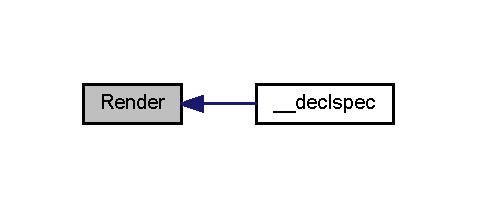
\includegraphics[width=229pt]{class_comet_engine_1_1_renderer_1_1_comet_engine_d_x_renderer_ac6fa4f62b984d0d34e785bd960255d71_icgraph}
\end{center}
\end{figure}


\subsection{멤버 데이터 문서화}
\mbox{\Hypertarget{class_comet_engine_1_1_renderer_1_1_comet_engine_d_x_renderer_af2bbff1b1d0120cc652b4f2198ddb04a}\label{class_comet_engine_1_1_renderer_1_1_comet_engine_d_x_renderer_af2bbff1b1d0120cc652b4f2198ddb04a}} 
\index{Comet\+Engine\+::\+Renderer\+::\+Comet\+Engine\+D\+X\+Renderer@{Comet\+Engine\+::\+Renderer\+::\+Comet\+Engine\+D\+X\+Renderer}!Instance@{Instance}}
\index{Instance@{Instance}!Comet\+Engine\+::\+Renderer\+::\+Comet\+Engine\+D\+X\+Renderer@{Comet\+Engine\+::\+Renderer\+::\+Comet\+Engine\+D\+X\+Renderer}}
\subsubsection{\texorpdfstring{Instance}{Instance}}
{\footnotesize\ttfamily \hyperlink{class_comet_engine_1_1_renderer_1_1_comet_engine_d_x_renderer}{Comet\+Engine\+D\+X\+Renderer} $\ast$ Instance = nullptr\hspace{0.3cm}{\ttfamily [static]}, {\ttfamily [private]}}



Comet\+Engine\+D\+X\+Renderer.\+h 파일의 24 번째 라인에서 정의되었습니다.

\mbox{\Hypertarget{class_comet_engine_1_1_renderer_1_1_comet_engine_d_x_renderer_a6ec5b124115c13d09e631e3245ba0264}\label{class_comet_engine_1_1_renderer_1_1_comet_engine_d_x_renderer_a6ec5b124115c13d09e631e3245ba0264}} 
\index{Comet\+Engine\+::\+Renderer\+::\+Comet\+Engine\+D\+X\+Renderer@{Comet\+Engine\+::\+Renderer\+::\+Comet\+Engine\+D\+X\+Renderer}!m\+\_\+h\+Render\+Target\+Hwnd@{m\+\_\+h\+Render\+Target\+Hwnd}}
\index{m\+\_\+h\+Render\+Target\+Hwnd@{m\+\_\+h\+Render\+Target\+Hwnd}!Comet\+Engine\+::\+Renderer\+::\+Comet\+Engine\+D\+X\+Renderer@{Comet\+Engine\+::\+Renderer\+::\+Comet\+Engine\+D\+X\+Renderer}}
\subsubsection{\texorpdfstring{m\+\_\+h\+Render\+Target\+Hwnd}{m\_hRenderTargetHwnd}}
{\footnotesize\ttfamily H\+W\+ND m\+\_\+h\+Render\+Target\+Hwnd\hspace{0.3cm}{\ttfamily [private]}}



Comet\+Engine\+D\+X\+Renderer.\+h 파일의 33 번째 라인에서 정의되었습니다.

\mbox{\Hypertarget{class_comet_engine_1_1_renderer_1_1_comet_engine_d_x_renderer_a4605315a46596f062351adb5071a334c}\label{class_comet_engine_1_1_renderer_1_1_comet_engine_d_x_renderer_a4605315a46596f062351adb5071a334c}} 
\index{Comet\+Engine\+::\+Renderer\+::\+Comet\+Engine\+D\+X\+Renderer@{Comet\+Engine\+::\+Renderer\+::\+Comet\+Engine\+D\+X\+Renderer}!m\+\_\+\+Is\+Debug\+Flag@{m\+\_\+\+Is\+Debug\+Flag}}
\index{m\+\_\+\+Is\+Debug\+Flag@{m\+\_\+\+Is\+Debug\+Flag}!Comet\+Engine\+::\+Renderer\+::\+Comet\+Engine\+D\+X\+Renderer@{Comet\+Engine\+::\+Renderer\+::\+Comet\+Engine\+D\+X\+Renderer}}
\subsubsection{\texorpdfstring{m\+\_\+\+Is\+Debug\+Flag}{m\_IsDebugFlag}}
{\footnotesize\ttfamily B\+O\+OL m\+\_\+\+Is\+Debug\+Flag\hspace{0.3cm}{\ttfamily [private]}}



Comet\+Engine\+D\+X\+Renderer.\+h 파일의 30 번째 라인에서 정의되었습니다.

\mbox{\Hypertarget{class_comet_engine_1_1_renderer_1_1_comet_engine_d_x_renderer_aa6179af78a783f7c0d77d6ea9b95abfb}\label{class_comet_engine_1_1_renderer_1_1_comet_engine_d_x_renderer_aa6179af78a783f7c0d77d6ea9b95abfb}} 
\index{Comet\+Engine\+::\+Renderer\+::\+Comet\+Engine\+D\+X\+Renderer@{Comet\+Engine\+::\+Renderer\+::\+Comet\+Engine\+D\+X\+Renderer}!m\+\_\+\+Is\+Full\+Screen@{m\+\_\+\+Is\+Full\+Screen}}
\index{m\+\_\+\+Is\+Full\+Screen@{m\+\_\+\+Is\+Full\+Screen}!Comet\+Engine\+::\+Renderer\+::\+Comet\+Engine\+D\+X\+Renderer@{Comet\+Engine\+::\+Renderer\+::\+Comet\+Engine\+D\+X\+Renderer}}
\subsubsection{\texorpdfstring{m\+\_\+\+Is\+Full\+Screen}{m\_IsFullScreen}}
{\footnotesize\ttfamily B\+O\+OL m\+\_\+\+Is\+Full\+Screen\hspace{0.3cm}{\ttfamily [private]}}



Comet\+Engine\+D\+X\+Renderer.\+h 파일의 31 번째 라인에서 정의되었습니다.

\mbox{\Hypertarget{class_comet_engine_1_1_renderer_1_1_comet_engine_d_x_renderer_ade12531fe5dd3f80e38d0baf16fe2c3f}\label{class_comet_engine_1_1_renderer_1_1_comet_engine_d_x_renderer_ade12531fe5dd3f80e38d0baf16fe2c3f}} 
\index{Comet\+Engine\+::\+Renderer\+::\+Comet\+Engine\+D\+X\+Renderer@{Comet\+Engine\+::\+Renderer\+::\+Comet\+Engine\+D\+X\+Renderer}!m\+\_\+\+Is\+M\+S\+AA@{m\+\_\+\+Is\+M\+S\+AA}}
\index{m\+\_\+\+Is\+M\+S\+AA@{m\+\_\+\+Is\+M\+S\+AA}!Comet\+Engine\+::\+Renderer\+::\+Comet\+Engine\+D\+X\+Renderer@{Comet\+Engine\+::\+Renderer\+::\+Comet\+Engine\+D\+X\+Renderer}}
\subsubsection{\texorpdfstring{m\+\_\+\+Is\+M\+S\+AA}{m\_IsMSAA}}
{\footnotesize\ttfamily B\+O\+OL m\+\_\+\+Is\+M\+S\+AA\hspace{0.3cm}{\ttfamily [private]}}



Comet\+Engine\+D\+X\+Renderer.\+h 파일의 29 번째 라인에서 정의되었습니다.

\mbox{\Hypertarget{class_comet_engine_1_1_renderer_1_1_comet_engine_d_x_renderer_aee26a00f9adfbcf0a5de3a91ec7e322d}\label{class_comet_engine_1_1_renderer_1_1_comet_engine_d_x_renderer_aee26a00f9adfbcf0a5de3a91ec7e322d}} 
\index{Comet\+Engine\+::\+Renderer\+::\+Comet\+Engine\+D\+X\+Renderer@{Comet\+Engine\+::\+Renderer\+::\+Comet\+Engine\+D\+X\+Renderer}!m\+\_\+u\+Msaa\+Level@{m\+\_\+u\+Msaa\+Level}}
\index{m\+\_\+u\+Msaa\+Level@{m\+\_\+u\+Msaa\+Level}!Comet\+Engine\+::\+Renderer\+::\+Comet\+Engine\+D\+X\+Renderer@{Comet\+Engine\+::\+Renderer\+::\+Comet\+Engine\+D\+X\+Renderer}}
\subsubsection{\texorpdfstring{m\+\_\+u\+Msaa\+Level}{m\_uMsaaLevel}}
{\footnotesize\ttfamily U\+I\+NT m\+\_\+u\+Msaa\+Level\hspace{0.3cm}{\ttfamily [private]}}



Comet\+Engine\+D\+X\+Renderer.\+h 파일의 35 번째 라인에서 정의되었습니다.

\mbox{\Hypertarget{class_comet_engine_1_1_renderer_1_1_comet_engine_d_x_renderer_af8f780a50f9325d3bad66c1ba49ed533}\label{class_comet_engine_1_1_renderer_1_1_comet_engine_d_x_renderer_af8f780a50f9325d3bad66c1ba49ed533}} 
\index{Comet\+Engine\+::\+Renderer\+::\+Comet\+Engine\+D\+X\+Renderer@{Comet\+Engine\+::\+Renderer\+::\+Comet\+Engine\+D\+X\+Renderer}!m\+\_\+u\+Render\+Height@{m\+\_\+u\+Render\+Height}}
\index{m\+\_\+u\+Render\+Height@{m\+\_\+u\+Render\+Height}!Comet\+Engine\+::\+Renderer\+::\+Comet\+Engine\+D\+X\+Renderer@{Comet\+Engine\+::\+Renderer\+::\+Comet\+Engine\+D\+X\+Renderer}}
\subsubsection{\texorpdfstring{m\+\_\+u\+Render\+Height}{m\_uRenderHeight}}
{\footnotesize\ttfamily U\+I\+NT m\+\_\+u\+Render\+Height\hspace{0.3cm}{\ttfamily [private]}}



Comet\+Engine\+D\+X\+Renderer.\+h 파일의 38 번째 라인에서 정의되었습니다.

\mbox{\Hypertarget{class_comet_engine_1_1_renderer_1_1_comet_engine_d_x_renderer_a00acfc4bfe2d732584f5ae0cb28186d8}\label{class_comet_engine_1_1_renderer_1_1_comet_engine_d_x_renderer_a00acfc4bfe2d732584f5ae0cb28186d8}} 
\index{Comet\+Engine\+::\+Renderer\+::\+Comet\+Engine\+D\+X\+Renderer@{Comet\+Engine\+::\+Renderer\+::\+Comet\+Engine\+D\+X\+Renderer}!m\+\_\+u\+Render\+Scale@{m\+\_\+u\+Render\+Scale}}
\index{m\+\_\+u\+Render\+Scale@{m\+\_\+u\+Render\+Scale}!Comet\+Engine\+::\+Renderer\+::\+Comet\+Engine\+D\+X\+Renderer@{Comet\+Engine\+::\+Renderer\+::\+Comet\+Engine\+D\+X\+Renderer}}
\subsubsection{\texorpdfstring{m\+\_\+u\+Render\+Scale}{m\_uRenderScale}}
{\footnotesize\ttfamily U\+I\+NT m\+\_\+u\+Render\+Scale\hspace{0.3cm}{\ttfamily [private]}}



Comet\+Engine\+D\+X\+Renderer.\+h 파일의 36 번째 라인에서 정의되었습니다.

\mbox{\Hypertarget{class_comet_engine_1_1_renderer_1_1_comet_engine_d_x_renderer_a3127a8dc19e4bd799fa7e1bfff28de11}\label{class_comet_engine_1_1_renderer_1_1_comet_engine_d_x_renderer_a3127a8dc19e4bd799fa7e1bfff28de11}} 
\index{Comet\+Engine\+::\+Renderer\+::\+Comet\+Engine\+D\+X\+Renderer@{Comet\+Engine\+::\+Renderer\+::\+Comet\+Engine\+D\+X\+Renderer}!m\+\_\+u\+Render\+Width@{m\+\_\+u\+Render\+Width}}
\index{m\+\_\+u\+Render\+Width@{m\+\_\+u\+Render\+Width}!Comet\+Engine\+::\+Renderer\+::\+Comet\+Engine\+D\+X\+Renderer@{Comet\+Engine\+::\+Renderer\+::\+Comet\+Engine\+D\+X\+Renderer}}
\subsubsection{\texorpdfstring{m\+\_\+u\+Render\+Width}{m\_uRenderWidth}}
{\footnotesize\ttfamily U\+I\+NT m\+\_\+u\+Render\+Width\hspace{0.3cm}{\ttfamily [private]}}



Comet\+Engine\+D\+X\+Renderer.\+h 파일의 37 번째 라인에서 정의되었습니다.

\mbox{\Hypertarget{class_comet_engine_1_1_renderer_1_1_comet_engine_d_x_renderer_a738b786f64e4fc6c9a2355f1cf9ae830}\label{class_comet_engine_1_1_renderer_1_1_comet_engine_d_x_renderer_a738b786f64e4fc6c9a2355f1cf9ae830}} 
\index{Comet\+Engine\+::\+Renderer\+::\+Comet\+Engine\+D\+X\+Renderer@{Comet\+Engine\+::\+Renderer\+::\+Comet\+Engine\+D\+X\+Renderer}!m\+Depth\+Stencil\+Buffer@{m\+Depth\+Stencil\+Buffer}}
\index{m\+Depth\+Stencil\+Buffer@{m\+Depth\+Stencil\+Buffer}!Comet\+Engine\+::\+Renderer\+::\+Comet\+Engine\+D\+X\+Renderer@{Comet\+Engine\+::\+Renderer\+::\+Comet\+Engine\+D\+X\+Renderer}}
\subsubsection{\texorpdfstring{m\+Depth\+Stencil\+Buffer}{mDepthStencilBuffer}}
{\footnotesize\ttfamily I\+D3\+D11\+Texture2D$\ast$ m\+Depth\+Stencil\+Buffer\hspace{0.3cm}{\ttfamily [private]}}



Comet\+Engine\+D\+X\+Renderer.\+h 파일의 46 번째 라인에서 정의되었습니다.

\mbox{\Hypertarget{class_comet_engine_1_1_renderer_1_1_comet_engine_d_x_renderer_a01cc1c2c77d9af90d45c250d51bcfa35}\label{class_comet_engine_1_1_renderer_1_1_comet_engine_d_x_renderer_a01cc1c2c77d9af90d45c250d51bcfa35}} 
\index{Comet\+Engine\+::\+Renderer\+::\+Comet\+Engine\+D\+X\+Renderer@{Comet\+Engine\+::\+Renderer\+::\+Comet\+Engine\+D\+X\+Renderer}!m\+Depth\+Stencil\+View@{m\+Depth\+Stencil\+View}}
\index{m\+Depth\+Stencil\+View@{m\+Depth\+Stencil\+View}!Comet\+Engine\+::\+Renderer\+::\+Comet\+Engine\+D\+X\+Renderer@{Comet\+Engine\+::\+Renderer\+::\+Comet\+Engine\+D\+X\+Renderer}}
\subsubsection{\texorpdfstring{m\+Depth\+Stencil\+View}{mDepthStencilView}}
{\footnotesize\ttfamily I\+D3\+D11\+Depth\+Stencil\+View$\ast$ m\+Depth\+Stencil\+View\hspace{0.3cm}{\ttfamily [private]}}



Comet\+Engine\+D\+X\+Renderer.\+h 파일의 45 번째 라인에서 정의되었습니다.

\mbox{\Hypertarget{class_comet_engine_1_1_renderer_1_1_comet_engine_d_x_renderer_ad38b8ad7fd1c747698a96256e75eb635}\label{class_comet_engine_1_1_renderer_1_1_comet_engine_d_x_renderer_ad38b8ad7fd1c747698a96256e75eb635}} 
\index{Comet\+Engine\+::\+Renderer\+::\+Comet\+Engine\+D\+X\+Renderer@{Comet\+Engine\+::\+Renderer\+::\+Comet\+Engine\+D\+X\+Renderer}!m\+D\+X\+Context@{m\+D\+X\+Context}}
\index{m\+D\+X\+Context@{m\+D\+X\+Context}!Comet\+Engine\+::\+Renderer\+::\+Comet\+Engine\+D\+X\+Renderer@{Comet\+Engine\+::\+Renderer\+::\+Comet\+Engine\+D\+X\+Renderer}}
\subsubsection{\texorpdfstring{m\+D\+X\+Context}{mDXContext}}
{\footnotesize\ttfamily I\+D3\+D11\+Device\+Context$\ast$ m\+D\+X\+Context\hspace{0.3cm}{\ttfamily [private]}}



Comet\+Engine\+D\+X\+Renderer.\+h 파일의 42 번째 라인에서 정의되었습니다.

\mbox{\Hypertarget{class_comet_engine_1_1_renderer_1_1_comet_engine_d_x_renderer_ac606b85554250d2e65a2aa9f10e6aa45}\label{class_comet_engine_1_1_renderer_1_1_comet_engine_d_x_renderer_ac606b85554250d2e65a2aa9f10e6aa45}} 
\index{Comet\+Engine\+::\+Renderer\+::\+Comet\+Engine\+D\+X\+Renderer@{Comet\+Engine\+::\+Renderer\+::\+Comet\+Engine\+D\+X\+Renderer}!m\+D\+X\+Device@{m\+D\+X\+Device}}
\index{m\+D\+X\+Device@{m\+D\+X\+Device}!Comet\+Engine\+::\+Renderer\+::\+Comet\+Engine\+D\+X\+Renderer@{Comet\+Engine\+::\+Renderer\+::\+Comet\+Engine\+D\+X\+Renderer}}
\subsubsection{\texorpdfstring{m\+D\+X\+Device}{mDXDevice}}
{\footnotesize\ttfamily I\+D3\+D11\+Device$\ast$ m\+D\+X\+Device\hspace{0.3cm}{\ttfamily [private]}}



Comet\+Engine\+D\+X\+Renderer.\+h 파일의 41 번째 라인에서 정의되었습니다.

\mbox{\Hypertarget{class_comet_engine_1_1_renderer_1_1_comet_engine_d_x_renderer_a109e138c97280440a0955d475441f49d}\label{class_comet_engine_1_1_renderer_1_1_comet_engine_d_x_renderer_a109e138c97280440a0955d475441f49d}} 
\index{Comet\+Engine\+::\+Renderer\+::\+Comet\+Engine\+D\+X\+Renderer@{Comet\+Engine\+::\+Renderer\+::\+Comet\+Engine\+D\+X\+Renderer}!m\+Render\+Target\+View@{m\+Render\+Target\+View}}
\index{m\+Render\+Target\+View@{m\+Render\+Target\+View}!Comet\+Engine\+::\+Renderer\+::\+Comet\+Engine\+D\+X\+Renderer@{Comet\+Engine\+::\+Renderer\+::\+Comet\+Engine\+D\+X\+Renderer}}
\subsubsection{\texorpdfstring{m\+Render\+Target\+View}{mRenderTargetView}}
{\footnotesize\ttfamily I\+D3\+D11\+Render\+Target\+View$\ast$ m\+Render\+Target\+View\hspace{0.3cm}{\ttfamily [private]}}



Comet\+Engine\+D\+X\+Renderer.\+h 파일의 44 번째 라인에서 정의되었습니다.

\mbox{\Hypertarget{class_comet_engine_1_1_renderer_1_1_comet_engine_d_x_renderer_a501ef6e0fe112727e82e727997af01c6}\label{class_comet_engine_1_1_renderer_1_1_comet_engine_d_x_renderer_a501ef6e0fe112727e82e727997af01c6}} 
\index{Comet\+Engine\+::\+Renderer\+::\+Comet\+Engine\+D\+X\+Renderer@{Comet\+Engine\+::\+Renderer\+::\+Comet\+Engine\+D\+X\+Renderer}!m\+Swap\+Chain@{m\+Swap\+Chain}}
\index{m\+Swap\+Chain@{m\+Swap\+Chain}!Comet\+Engine\+::\+Renderer\+::\+Comet\+Engine\+D\+X\+Renderer@{Comet\+Engine\+::\+Renderer\+::\+Comet\+Engine\+D\+X\+Renderer}}
\subsubsection{\texorpdfstring{m\+Swap\+Chain}{mSwapChain}}
{\footnotesize\ttfamily I\+D\+X\+G\+I\+Swap\+Chain$\ast$ m\+Swap\+Chain\hspace{0.3cm}{\ttfamily [private]}}



Comet\+Engine\+D\+X\+Renderer.\+h 파일의 43 번째 라인에서 정의되었습니다.



이 클래스에 대한 문서화 페이지는 다음의 파일들로부터 생성되었습니다.\+:\begin{DoxyCompactItemize}
\item 
Comet\+Engine\+Client/\+Comet\+Engine\+Renderer/\+Renderer/\hyperlink{_comet_engine_d_x_renderer_8h}{Comet\+Engine\+D\+X\+Renderer.\+h}\item 
Comet\+Engine\+Client/\+Comet\+Engine\+Renderer/\+Renderer/\hyperlink{_comet_engine_d_x_renderer_8cpp}{Comet\+Engine\+D\+X\+Renderer.\+cpp}\end{DoxyCompactItemize}

\hypertarget{class_comet_engine_1_1_comet_engine_win32}{}\section{Comet\+Engine\+Win32 클래스 참조}
\label{class_comet_engine_1_1_comet_engine_win32}\index{Comet\+Engine\+Win32@{Comet\+Engine\+Win32}}


{\ttfamily \#include $<$Comet\+Engine\+Win32.\+h$>$}



Comet\+Engine\+Win32에 대한 협력 다이어그램\+:\nopagebreak
\begin{figure}[H]
\begin{center}
\leavevmode
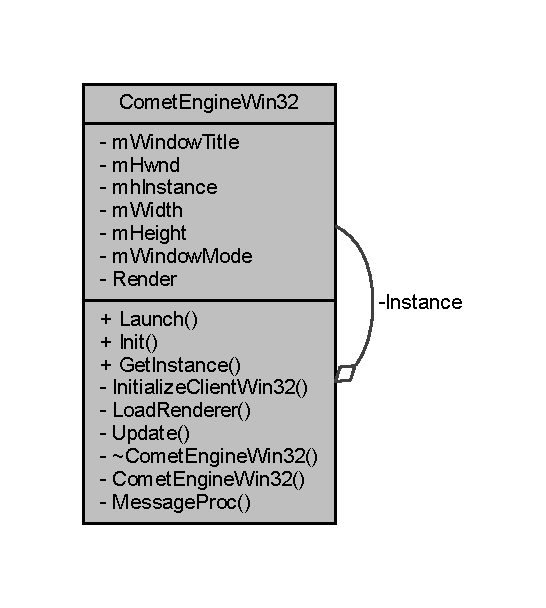
\includegraphics[width=262pt]{class_comet_engine_1_1_comet_engine_win32__coll__graph}
\end{center}
\end{figure}
\subsection*{Public 멤버 함수}
\begin{DoxyCompactItemize}
\item 
void \hyperlink{class_comet_engine_1_1_comet_engine_win32_abe9b413e3c019ccee4f87ab0071c5aad}{Launch} ()
\item 
bool \hyperlink{class_comet_engine_1_1_comet_engine_win32_a1663bd9ecefc952f3f74065a592ad663}{Init} (wchar\+\_\+t $\ast$Window\+Title, int W\+Idth, int \hyperlink{_d_l_l_comet_engine_win32_8cpp_afd53bc431b967813e00ae3cfecd5c548}{Height}, \hyperlink{namespace_comet_engine_abdc5ec13bf1dfb1d26eb0bcc9da0ddad}{W\+I\+N\+D\+O\+W\+\_\+\+M\+O\+DE} \hyperlink{_d_l_l_comet_engine_win32_8cpp_a319b6c977f6b5f638f8246c67a367768}{Window\+Mode}, H\+I\+N\+S\+T\+A\+N\+CE \hyperlink{_d_l_l_comet_engine_win32_8cpp_a5fb685beb2aed3ecdbad03b352111398}{h\+Instance}, L\+P\+S\+TR \hyperlink{_d_l_l_comet_engine_win32_8cpp_af1ff5ad877f6069d41720b03c7769227}{lp\+Cmd\+Line})
\end{DoxyCompactItemize}
\subsection*{정적 Public 멤버 함수}
\begin{DoxyCompactItemize}
\item 
static \hyperlink{class_comet_engine_1_1_comet_engine_win32}{Comet\+Engine\+Win32} $\ast$ \hyperlink{class_comet_engine_1_1_comet_engine_win32_af96d04b2fa84467a5342e290690e40fb}{Get\+Instance} ()
\end{DoxyCompactItemize}
\subsection*{Private 타입}
\begin{DoxyCompactItemize}
\item 
typedef void($\ast$ \hyperlink{class_comet_engine_1_1_comet_engine_win32_a97e4f6f1bfb397686ef973fe8bd42abf}{Render\+\_\+func}) (float dt)
\end{DoxyCompactItemize}
\subsection*{Private 멤버 함수}
\begin{DoxyCompactItemize}
\item 
bool \hyperlink{class_comet_engine_1_1_comet_engine_win32_a9f5ac1f01164dfdb7f752e6b4f77e80a}{Initialize\+Client\+Win32} (L\+P\+S\+TR \hyperlink{_d_l_l_comet_engine_win32_8cpp_af1ff5ad877f6069d41720b03c7769227}{lp\+Cmd\+Line})
\item 
bool \hyperlink{class_comet_engine_1_1_comet_engine_win32_a35f30fb8a7991557468d2fc3b25ff0b7}{Load\+Renderer} ()
\item 
void \hyperlink{class_comet_engine_1_1_comet_engine_win32_a5ceefb272acf4d0adb4964ec29e5996e}{Update} (float delta)
\item 
\hyperlink{class_comet_engine_1_1_comet_engine_win32_adc512ee25a2e71f894d254ae3b293ff0}{$\sim$\+Comet\+Engine\+Win32} ()
\item 
\hyperlink{class_comet_engine_1_1_comet_engine_win32_a62369ca325b16b42ad77a4f1523e4356}{Comet\+Engine\+Win32} ()
\end{DoxyCompactItemize}
\subsection*{정적 Private 멤버 함수}
\begin{DoxyCompactItemize}
\item 
static H\+R\+E\+S\+U\+LT C\+A\+L\+L\+B\+A\+CK \hyperlink{class_comet_engine_1_1_comet_engine_win32_a69f7f5121282027943c96964bb85ef85}{Message\+Proc} (H\+W\+ND h\+Wnd, U\+I\+NT i\+Message, W\+P\+A\+R\+AM w\+Param, L\+P\+A\+R\+AM l\+Param)
\end{DoxyCompactItemize}
\subsection*{Private 속성}
\begin{DoxyCompactItemize}
\item 
wchar\+\_\+t $\ast$ \hyperlink{class_comet_engine_1_1_comet_engine_win32_a63ee29dd5d917889a0e7b644fea26d06}{m\+Window\+Title}
\item 
H\+W\+ND \hyperlink{class_comet_engine_1_1_comet_engine_win32_a31c6576456c4bfea9672c5198aa18460}{m\+Hwnd}
\item 
H\+I\+N\+S\+T\+A\+N\+CE \hyperlink{class_comet_engine_1_1_comet_engine_win32_a699a17c72a7b5416a8966df051f9c752}{mh\+Instance}
\item 
U\+I\+NT \hyperlink{class_comet_engine_1_1_comet_engine_win32_a954be7feb8f6558f86a08a30d640013e}{m\+Width}
\item 
U\+I\+NT \hyperlink{class_comet_engine_1_1_comet_engine_win32_ae5ce9d2610ee7e9675a4ecc74b0c9492}{m\+Height}
\item 
\hyperlink{namespace_comet_engine_abdc5ec13bf1dfb1d26eb0bcc9da0ddad}{W\+I\+N\+D\+O\+W\+\_\+\+M\+O\+DE} \hyperlink{class_comet_engine_1_1_comet_engine_win32_a31fa5cdc3ed0a81919f9ae7ec61844d1}{m\+Window\+Mode}
\item 
\hyperlink{class_comet_engine_1_1_comet_engine_win32_a97e4f6f1bfb397686ef973fe8bd42abf}{Render\+\_\+func} \hyperlink{class_comet_engine_1_1_comet_engine_win32_a805efc6c9b43dd5daa64e3c1392d18b3}{Render}
\end{DoxyCompactItemize}
\subsection*{정적 Private 속성}
\begin{DoxyCompactItemize}
\item 
static \hyperlink{class_comet_engine_1_1_comet_engine_win32}{Comet\+Engine\+Win32} $\ast$ \hyperlink{class_comet_engine_1_1_comet_engine_win32_ac980c50873d6df828203b639e543de14}{Instance} = N\+U\+LL
\end{DoxyCompactItemize}


\subsection{상세한 설명}


Comet\+Engine\+Win32.\+h 파일의 18 번째 라인에서 정의되었습니다.



\subsection{멤버 타입정의 문서화}
\mbox{\Hypertarget{class_comet_engine_1_1_comet_engine_win32_a97e4f6f1bfb397686ef973fe8bd42abf}\label{class_comet_engine_1_1_comet_engine_win32_a97e4f6f1bfb397686ef973fe8bd42abf}} 
\index{Comet\+Engine\+::\+Comet\+Engine\+Win32@{Comet\+Engine\+::\+Comet\+Engine\+Win32}!Render\+\_\+func@{Render\+\_\+func}}
\index{Render\+\_\+func@{Render\+\_\+func}!Comet\+Engine\+::\+Comet\+Engine\+Win32@{Comet\+Engine\+::\+Comet\+Engine\+Win32}}
\subsubsection{\texorpdfstring{Render\+\_\+func}{Render\_func}}
{\footnotesize\ttfamily typedef void($\ast$ Render\+\_\+func) (float dt)\hspace{0.3cm}{\ttfamily [private]}}



Comet\+Engine\+Win32.\+h 파일의 20 번째 라인에서 정의되었습니다.



\subsection{생성자 \& 소멸자 문서화}
\mbox{\Hypertarget{class_comet_engine_1_1_comet_engine_win32_adc512ee25a2e71f894d254ae3b293ff0}\label{class_comet_engine_1_1_comet_engine_win32_adc512ee25a2e71f894d254ae3b293ff0}} 
\index{Comet\+Engine\+::\+Comet\+Engine\+Win32@{Comet\+Engine\+::\+Comet\+Engine\+Win32}!````~Comet\+Engine\+Win32@{$\sim$\+Comet\+Engine\+Win32}}
\index{````~Comet\+Engine\+Win32@{$\sim$\+Comet\+Engine\+Win32}!Comet\+Engine\+::\+Comet\+Engine\+Win32@{Comet\+Engine\+::\+Comet\+Engine\+Win32}}
\subsubsection{\texorpdfstring{$\sim$\+Comet\+Engine\+Win32()}{~CometEngineWin32()}}
{\footnotesize\ttfamily $\sim$\hyperlink{class_comet_engine_1_1_comet_engine_win32}{Comet\+Engine\+Win32} (\begin{DoxyParamCaption}{ }\end{DoxyParamCaption})\hspace{0.3cm}{\ttfamily [private]}}



Comet\+Engine\+Win32.\+cpp 파일의 12 번째 라인에서 정의되었습니다.


\begin{DoxyCode}
13 \{
14 
15     \textcolor{keyword}{delete} \hyperlink{class_comet_engine_1_1_comet_engine_win32_ac980c50873d6df828203b639e543de14}{Instance};
16 \}
\end{DoxyCode}
\mbox{\Hypertarget{class_comet_engine_1_1_comet_engine_win32_a62369ca325b16b42ad77a4f1523e4356}\label{class_comet_engine_1_1_comet_engine_win32_a62369ca325b16b42ad77a4f1523e4356}} 
\index{Comet\+Engine\+::\+Comet\+Engine\+Win32@{Comet\+Engine\+::\+Comet\+Engine\+Win32}!Comet\+Engine\+Win32@{Comet\+Engine\+Win32}}
\index{Comet\+Engine\+Win32@{Comet\+Engine\+Win32}!Comet\+Engine\+::\+Comet\+Engine\+Win32@{Comet\+Engine\+::\+Comet\+Engine\+Win32}}
\subsubsection{\texorpdfstring{Comet\+Engine\+Win32()}{CometEngineWin32()}}
{\footnotesize\ttfamily \hyperlink{class_comet_engine_1_1_comet_engine_win32}{Comet\+Engine\+Win32} (\begin{DoxyParamCaption}{ }\end{DoxyParamCaption})\hspace{0.3cm}{\ttfamily [private]}}



Comet\+Engine\+Win32.\+cpp 파일의 7 번째 라인에서 정의되었습니다.


\begin{DoxyCode}
8 \{
9 
10 \}
\end{DoxyCode}
이 함수를 호출하는 함수들에 대한 그래프입니다.\+:\nopagebreak
\begin{figure}[H]
\begin{center}
\leavevmode
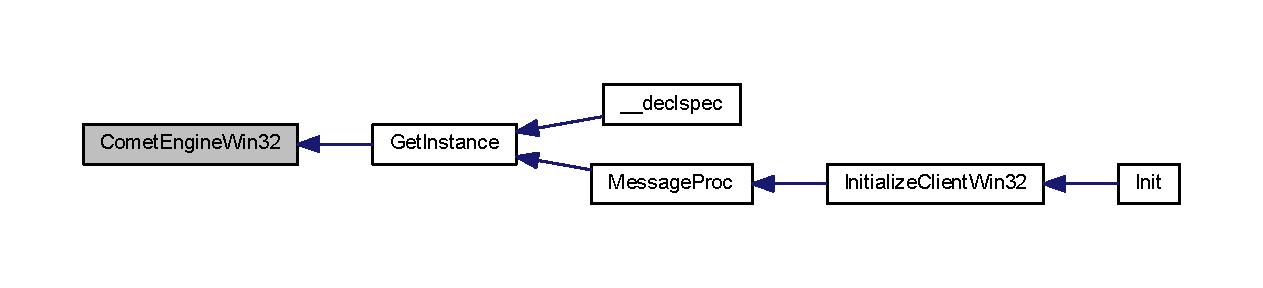
\includegraphics[width=350pt]{class_comet_engine_1_1_comet_engine_win32_a62369ca325b16b42ad77a4f1523e4356_icgraph}
\end{center}
\end{figure}


\subsection{멤버 함수 문서화}
\mbox{\Hypertarget{class_comet_engine_1_1_comet_engine_win32_af96d04b2fa84467a5342e290690e40fb}\label{class_comet_engine_1_1_comet_engine_win32_af96d04b2fa84467a5342e290690e40fb}} 
\index{Comet\+Engine\+::\+Comet\+Engine\+Win32@{Comet\+Engine\+::\+Comet\+Engine\+Win32}!Get\+Instance@{Get\+Instance}}
\index{Get\+Instance@{Get\+Instance}!Comet\+Engine\+::\+Comet\+Engine\+Win32@{Comet\+Engine\+::\+Comet\+Engine\+Win32}}
\subsubsection{\texorpdfstring{Get\+Instance()}{GetInstance()}}
{\footnotesize\ttfamily \hyperlink{class_comet_engine_1_1_comet_engine_win32}{Comet\+Engine\+Win32} $\ast$ Get\+Instance (\begin{DoxyParamCaption}{ }\end{DoxyParamCaption})\hspace{0.3cm}{\ttfamily [static]}}



Comet\+Engine\+Win32.\+cpp 파일의 18 번째 라인에서 정의되었습니다.


\begin{DoxyCode}
19 \{
20     \textcolor{keywordflow}{if} (\hyperlink{class_comet_engine_1_1_comet_engine_win32_ac980c50873d6df828203b639e543de14}{Instance} == NULL)
21         \hyperlink{class_comet_engine_1_1_comet_engine_win32_ac980c50873d6df828203b639e543de14}{Instance} = \textcolor{keyword}{new} \hyperlink{class_comet_engine_1_1_comet_engine_win32_a62369ca325b16b42ad77a4f1523e4356}{CometEngineWin32}();
22     \textcolor{keywordflow}{return} \hyperlink{class_comet_engine_1_1_comet_engine_win32_ac980c50873d6df828203b639e543de14}{Instance};
23 \}
\end{DoxyCode}
이 함수 내부에서 호출하는 함수들에 대한 그래프입니다.\+:\nopagebreak
\begin{figure}[H]
\begin{center}
\leavevmode
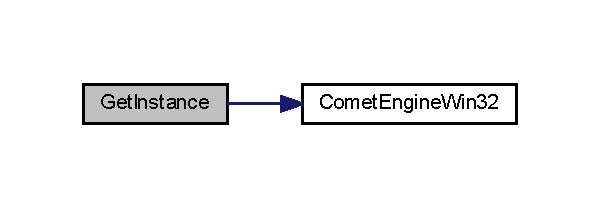
\includegraphics[width=288pt]{class_comet_engine_1_1_comet_engine_win32_af96d04b2fa84467a5342e290690e40fb_cgraph}
\end{center}
\end{figure}
이 함수를 호출하는 함수들에 대한 그래프입니다.\+:\nopagebreak
\begin{figure}[H]
\begin{center}
\leavevmode
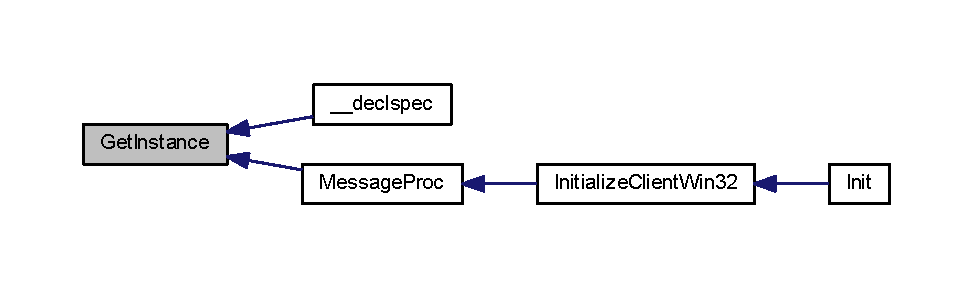
\includegraphics[width=350pt]{class_comet_engine_1_1_comet_engine_win32_af96d04b2fa84467a5342e290690e40fb_icgraph}
\end{center}
\end{figure}
\mbox{\Hypertarget{class_comet_engine_1_1_comet_engine_win32_a1663bd9ecefc952f3f74065a592ad663}\label{class_comet_engine_1_1_comet_engine_win32_a1663bd9ecefc952f3f74065a592ad663}} 
\index{Comet\+Engine\+::\+Comet\+Engine\+Win32@{Comet\+Engine\+::\+Comet\+Engine\+Win32}!Init@{Init}}
\index{Init@{Init}!Comet\+Engine\+::\+Comet\+Engine\+Win32@{Comet\+Engine\+::\+Comet\+Engine\+Win32}}
\subsubsection{\texorpdfstring{Init()}{Init()}}
{\footnotesize\ttfamily bool Init (\begin{DoxyParamCaption}\item[{wchar\+\_\+t $\ast$}]{Window\+Title,  }\item[{int}]{W\+Idth,  }\item[{int}]{Height,  }\item[{\hyperlink{namespace_comet_engine_abdc5ec13bf1dfb1d26eb0bcc9da0ddad}{W\+I\+N\+D\+O\+W\+\_\+\+M\+O\+DE}}]{Window\+Mode,  }\item[{H\+I\+N\+S\+T\+A\+N\+CE}]{h\+Instance,  }\item[{L\+P\+S\+TR}]{lp\+Cmd\+Line }\end{DoxyParamCaption})}



Comet\+Engine\+Win32.\+cpp 파일의 49 번째 라인에서 정의되었습니다.


\begin{DoxyCode}
50 \{
51     \hyperlink{class_comet_engine_1_1_comet_engine_win32_a63ee29dd5d917889a0e7b644fea26d06}{mWindowTitle} = WindowTitle;
52     \hyperlink{class_comet_engine_1_1_comet_engine_win32_a954be7feb8f6558f86a08a30d640013e}{mWidth}         = \hyperlink{_d_l_l_comet_engine_win32_8cpp_abbe7749c3b402f7dfe64f936774cfcd4}{Width};
53     \hyperlink{class_comet_engine_1_1_comet_engine_win32_ae5ce9d2610ee7e9675a4ecc74b0c9492}{mHeight}       = \hyperlink{_d_l_l_comet_engine_win32_8cpp_afd53bc431b967813e00ae3cfecd5c548}{Height};
54     \hyperlink{class_comet_engine_1_1_comet_engine_win32_a31fa5cdc3ed0a81919f9ae7ec61844d1}{mWindowMode}  = \hyperlink{_d_l_l_comet_engine_win32_8cpp_a319b6c977f6b5f638f8246c67a367768}{WindowMode};
55     \hyperlink{class_comet_engine_1_1_comet_engine_win32_a699a17c72a7b5416a8966df051f9c752}{mhInstance}     = \hyperlink{_d_l_l_comet_engine_win32_8cpp_a5fb685beb2aed3ecdbad03b352111398}{hInstance};
56     \textcolor{keywordflow}{return} \hyperlink{class_comet_engine_1_1_comet_engine_win32_a9f5ac1f01164dfdb7f752e6b4f77e80a}{InitializeClientWin32}(\hyperlink{_d_l_l_comet_engine_win32_8cpp_af1ff5ad877f6069d41720b03c7769227}{lpCmdLine}) && 
      \hyperlink{class_comet_engine_1_1_comet_engine_win32_a35f30fb8a7991557468d2fc3b25ff0b7}{LoadRenderer}();
57 \}
\end{DoxyCode}
이 함수 내부에서 호출하는 함수들에 대한 그래프입니다.\+:\nopagebreak
\begin{figure}[H]
\begin{center}
\leavevmode
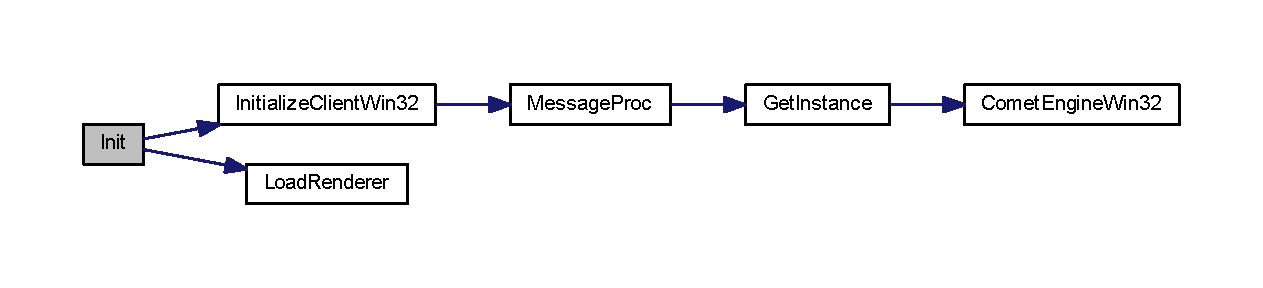
\includegraphics[width=350pt]{class_comet_engine_1_1_comet_engine_win32_a1663bd9ecefc952f3f74065a592ad663_cgraph}
\end{center}
\end{figure}
\mbox{\Hypertarget{class_comet_engine_1_1_comet_engine_win32_a9f5ac1f01164dfdb7f752e6b4f77e80a}\label{class_comet_engine_1_1_comet_engine_win32_a9f5ac1f01164dfdb7f752e6b4f77e80a}} 
\index{Comet\+Engine\+::\+Comet\+Engine\+Win32@{Comet\+Engine\+::\+Comet\+Engine\+Win32}!Initialize\+Client\+Win32@{Initialize\+Client\+Win32}}
\index{Initialize\+Client\+Win32@{Initialize\+Client\+Win32}!Comet\+Engine\+::\+Comet\+Engine\+Win32@{Comet\+Engine\+::\+Comet\+Engine\+Win32}}
\subsubsection{\texorpdfstring{Initialize\+Client\+Win32()}{InitializeClientWin32()}}
{\footnotesize\ttfamily bool Initialize\+Client\+Win32 (\begin{DoxyParamCaption}\item[{L\+P\+S\+TR}]{lp\+Cmd\+Line }\end{DoxyParamCaption})\hspace{0.3cm}{\ttfamily [private]}}



Comet\+Engine\+Win32.\+cpp 파일의 58 번째 라인에서 정의되었습니다.


\begin{DoxyCode}
59 \{
60     WNDCLASSEX wndx = \{ 0 \};
61     wndx.cbClsExtra = 0;
62     wndx.cbWndExtra = 0;
63     wndx.cbSize = \textcolor{keyword}{sizeof}(WNDCLASSEX);
64     wndx.style = CS\_HREDRAW | CS\_VREDRAW;
65     wndx.hInstance = \hyperlink{class_comet_engine_1_1_comet_engine_win32_a699a17c72a7b5416a8966df051f9c752}{mhInstance};
66     wndx.lpfnWndProc = (WNDPROC)\hyperlink{class_comet_engine_1_1_comet_engine_win32_a69f7f5121282027943c96964bb85ef85}{MessageProc};
67     wndx.hIcon = LoadIcon(NULL, IDI\_APPLICATION);
68     wndx.hIconSm = LoadIcon(NULL, IDI\_APPLICATION);
69     wndx.hCursor = LoadCursor(NULL, IDC\_ARROW);
70     wndx.hbrBackground = (HBRUSH)GetStockObject(NULL\_BRUSH);
71     wndx.lpszMenuName = NULL;
72     wndx.lpszClassName = L\textcolor{stringliteral}{"CometEngineApplication"};
73 
74     \textcolor{keywordflow}{if} (!RegisterClassEx(&wndx))
75     \{
76         OutputDebugString(L\textcolor{stringliteral}{"\(\backslash\)n Create Window FAILED"});
77         OutputDebugString(std::to\_wstring(GetLastError()).c\_str());
78 
79         \textcolor{keywordflow}{return} \textcolor{keyword}{false};
80     \}
81 
82      \hyperlink{class_comet_engine_1_1_comet_engine_win32_a31c6576456c4bfea9672c5198aa18460}{mHwnd} = CreateWindow(L\textcolor{stringliteral}{"CometEngineApplication"}, \hyperlink{class_comet_engine_1_1_comet_engine_win32_a63ee29dd5d917889a0e7b644fea26d06}{mWindowTitle}, WS\_OVERLAPPEDWINDOW,
83         CW\_USEDEFAULT, CW\_USEDEFAULT, \hyperlink{class_comet_engine_1_1_comet_engine_win32_a954be7feb8f6558f86a08a30d640013e}{mWidth}, \hyperlink{class_comet_engine_1_1_comet_engine_win32_ae5ce9d2610ee7e9675a4ecc74b0c9492}{mHeight},
84         NULL, (HMENU)NULL, \hyperlink{class_comet_engine_1_1_comet_engine_win32_a699a17c72a7b5416a8966df051f9c752}{mhInstance}, NULL);
85 
86     \textcolor{keywordflow}{if} (\hyperlink{class_comet_engine_1_1_comet_engine_win32_a31fa5cdc3ed0a81919f9ae7ec61844d1}{mWindowMode} == \hyperlink{namespace_comet_engine_abdc5ec13bf1dfb1d26eb0bcc9da0ddada2fcf3c9ce3f39ff118fc4e667c4e2cc6}{WINDOW\_MODE::NO\_BORDER})
87     \{
88         SetWindowLong(\hyperlink{class_comet_engine_1_1_comet_engine_win32_a31c6576456c4bfea9672c5198aa18460}{mHwnd}, GWL\_STYLE, 0);
89     \}
90 
91     ShowWindow(\hyperlink{class_comet_engine_1_1_comet_engine_win32_a31c6576456c4bfea9672c5198aa18460}{mHwnd}, SW\_SHOW);
92 
93     \textcolor{keywordflow}{return} \textcolor{keyword}{true};
94 
95     
96 \}
\end{DoxyCode}
이 함수 내부에서 호출하는 함수들에 대한 그래프입니다.\+:\nopagebreak
\begin{figure}[H]
\begin{center}
\leavevmode
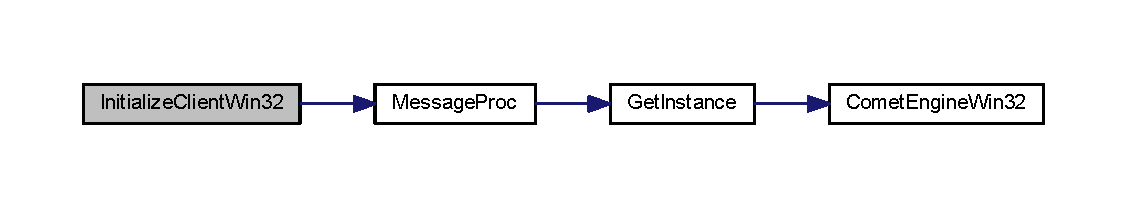
\includegraphics[width=350pt]{class_comet_engine_1_1_comet_engine_win32_a9f5ac1f01164dfdb7f752e6b4f77e80a_cgraph}
\end{center}
\end{figure}
이 함수를 호출하는 함수들에 대한 그래프입니다.\+:\nopagebreak
\begin{figure}[H]
\begin{center}
\leavevmode
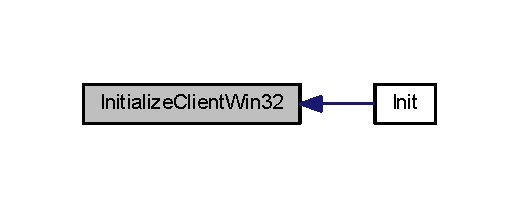
\includegraphics[width=249pt]{class_comet_engine_1_1_comet_engine_win32_a9f5ac1f01164dfdb7f752e6b4f77e80a_icgraph}
\end{center}
\end{figure}
\mbox{\Hypertarget{class_comet_engine_1_1_comet_engine_win32_abe9b413e3c019ccee4f87ab0071c5aad}\label{class_comet_engine_1_1_comet_engine_win32_abe9b413e3c019ccee4f87ab0071c5aad}} 
\index{Comet\+Engine\+::\+Comet\+Engine\+Win32@{Comet\+Engine\+::\+Comet\+Engine\+Win32}!Launch@{Launch}}
\index{Launch@{Launch}!Comet\+Engine\+::\+Comet\+Engine\+Win32@{Comet\+Engine\+::\+Comet\+Engine\+Win32}}
\subsubsection{\texorpdfstring{Launch()}{Launch()}}
{\footnotesize\ttfamily void Launch (\begin{DoxyParamCaption}{ }\end{DoxyParamCaption})}



Comet\+Engine\+Win32.\+cpp 파일의 98 번째 라인에서 정의되었습니다.


\begin{DoxyCode}
99 \{
100     MSG msg = \{ 0, \};
101     \textcolor{keywordflow}{while} (WM\_QUIT != msg.message)
102     \{
103         \textcolor{keywordflow}{if} (PeekMessage(&msg, NULL, NULL, NULL, PM\_REMOVE))
104         \{
105             TranslateMessage(&msg);
106             DispatchMessage(&msg);
107         \}
108         \textcolor{keywordflow}{else}
109         \{
110             \hyperlink{class_comet_engine_1_1_comet_engine_win32_a5ceefb272acf4d0adb4964ec29e5996e}{Update}(0);
111 
112         \}
113     \}
114     PostQuitMessage(0);
115 \}
\end{DoxyCode}
이 함수 내부에서 호출하는 함수들에 대한 그래프입니다.\+:\nopagebreak
\begin{figure}[H]
\begin{center}
\leavevmode
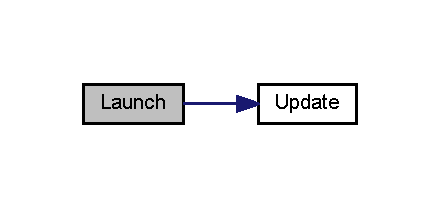
\includegraphics[width=211pt]{class_comet_engine_1_1_comet_engine_win32_abe9b413e3c019ccee4f87ab0071c5aad_cgraph}
\end{center}
\end{figure}
이 함수를 호출하는 함수들에 대한 그래프입니다.\+:\nopagebreak
\begin{figure}[H]
\begin{center}
\leavevmode
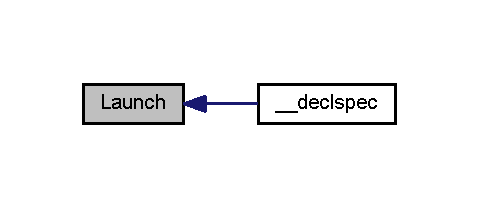
\includegraphics[width=230pt]{class_comet_engine_1_1_comet_engine_win32_abe9b413e3c019ccee4f87ab0071c5aad_icgraph}
\end{center}
\end{figure}
\mbox{\Hypertarget{class_comet_engine_1_1_comet_engine_win32_a35f30fb8a7991557468d2fc3b25ff0b7}\label{class_comet_engine_1_1_comet_engine_win32_a35f30fb8a7991557468d2fc3b25ff0b7}} 
\index{Comet\+Engine\+::\+Comet\+Engine\+Win32@{Comet\+Engine\+::\+Comet\+Engine\+Win32}!Load\+Renderer@{Load\+Renderer}}
\index{Load\+Renderer@{Load\+Renderer}!Comet\+Engine\+::\+Comet\+Engine\+Win32@{Comet\+Engine\+::\+Comet\+Engine\+Win32}}
\subsubsection{\texorpdfstring{Load\+Renderer()}{LoadRenderer()}}
{\footnotesize\ttfamily bool Load\+Renderer (\begin{DoxyParamCaption}{ }\end{DoxyParamCaption})\hspace{0.3cm}{\ttfamily [private]}}



Comet\+Engine\+Win32.\+cpp 파일의 117 번째 라인에서 정의되었습니다.


\begin{DoxyCode}
118 \{
119     HINSTANCE renderer = LoadLibrary(L\textcolor{stringliteral}{"CometEngineDXRenderer.dll"});
120     
121     \textcolor{keywordflow}{if} (renderer == NULL)
122         \textcolor{keywordflow}{return} \textcolor{keyword}{false};
123     \hyperlink{class_comet_engine_1_1_comet_engine_win32_a805efc6c9b43dd5daa64e3c1392d18b3}{Render} = (\hyperlink{class_comet_engine_1_1_comet_engine_win32_a97e4f6f1bfb397686ef973fe8bd42abf}{Render\_func})GetProcAddress(renderer, \textcolor{stringliteral}{"Render"});
124     \textcolor{keywordflow}{if} (\hyperlink{class_comet_engine_1_1_comet_engine_win32_a805efc6c9b43dd5daa64e3c1392d18b3}{Render} == NULL)
125         \textcolor{keywordflow}{return} \textcolor{keyword}{false};
126 \textcolor{comment}{//  if (\_\_DEBUG\_\_) }
127         
128     
129     \textcolor{keywordflow}{return} \textcolor{keyword}{true};
130 \}
\end{DoxyCode}
이 함수를 호출하는 함수들에 대한 그래프입니다.\+:\nopagebreak
\begin{figure}[H]
\begin{center}
\leavevmode
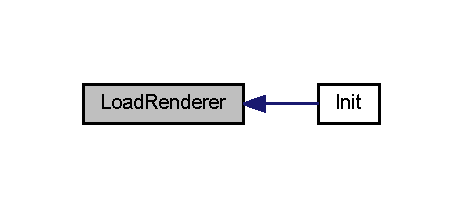
\includegraphics[width=222pt]{class_comet_engine_1_1_comet_engine_win32_a35f30fb8a7991557468d2fc3b25ff0b7_icgraph}
\end{center}
\end{figure}
\mbox{\Hypertarget{class_comet_engine_1_1_comet_engine_win32_a69f7f5121282027943c96964bb85ef85}\label{class_comet_engine_1_1_comet_engine_win32_a69f7f5121282027943c96964bb85ef85}} 
\index{Comet\+Engine\+::\+Comet\+Engine\+Win32@{Comet\+Engine\+::\+Comet\+Engine\+Win32}!Message\+Proc@{Message\+Proc}}
\index{Message\+Proc@{Message\+Proc}!Comet\+Engine\+::\+Comet\+Engine\+Win32@{Comet\+Engine\+::\+Comet\+Engine\+Win32}}
\subsubsection{\texorpdfstring{Message\+Proc()}{MessageProc()}}
{\footnotesize\ttfamily H\+R\+E\+S\+U\+LT C\+A\+L\+L\+B\+A\+CK Message\+Proc (\begin{DoxyParamCaption}\item[{H\+W\+ND}]{h\+Wnd,  }\item[{U\+I\+NT}]{i\+Message,  }\item[{W\+P\+A\+R\+AM}]{w\+Param,  }\item[{L\+P\+A\+R\+AM}]{l\+Param }\end{DoxyParamCaption})\hspace{0.3cm}{\ttfamily [static]}, {\ttfamily [private]}}



Comet\+Engine\+Win32.\+cpp 파일의 25 번째 라인에서 정의되었습니다.


\begin{DoxyCode}
26 \{
27     \textcolor{keywordflow}{switch} (iMessage)
28     \{
29     \textcolor{keywordflow}{case} WM\_CLOSE:
30         DestroyWindow(hWnd);
31         \textcolor{keywordflow}{return} 0;
32     \textcolor{keywordflow}{case} WM\_DESTROY:
33         PostQuitMessage(0);
34         \textcolor{keywordflow}{return} 0;
35     \textcolor{keywordflow}{default}:
36         \textcolor{keywordflow}{return} (HRESULT)DefWindowProc(hWnd, iMessage, wParam, lParam);
37     \}
38     \hyperlink{class_comet_engine_1_1_comet_engine_win32_af96d04b2fa84467a5342e290690e40fb}{CometEngineWin32::GetInstance}()->\hyperlink{class_comet_engine_1_1_comet_engine_win32_a805efc6c9b43dd5daa64e3c1392d18b3}{Render}(0);
39     \textcolor{keywordflow}{return} 0;
40 \}
\end{DoxyCode}
이 함수 내부에서 호출하는 함수들에 대한 그래프입니다.\+:\nopagebreak
\begin{figure}[H]
\begin{center}
\leavevmode
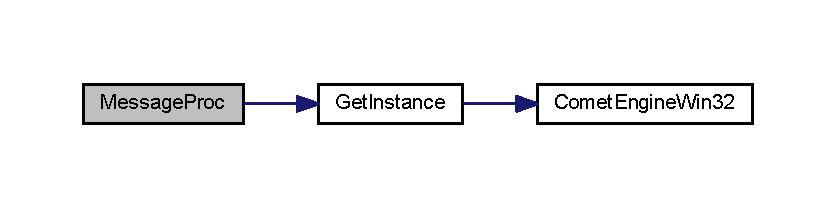
\includegraphics[width=350pt]{class_comet_engine_1_1_comet_engine_win32_a69f7f5121282027943c96964bb85ef85_cgraph}
\end{center}
\end{figure}
이 함수를 호출하는 함수들에 대한 그래프입니다.\+:\nopagebreak
\begin{figure}[H]
\begin{center}
\leavevmode
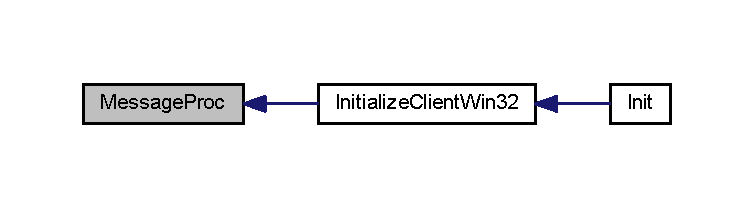
\includegraphics[width=350pt]{class_comet_engine_1_1_comet_engine_win32_a69f7f5121282027943c96964bb85ef85_icgraph}
\end{center}
\end{figure}
\mbox{\Hypertarget{class_comet_engine_1_1_comet_engine_win32_a5ceefb272acf4d0adb4964ec29e5996e}\label{class_comet_engine_1_1_comet_engine_win32_a5ceefb272acf4d0adb4964ec29e5996e}} 
\index{Comet\+Engine\+::\+Comet\+Engine\+Win32@{Comet\+Engine\+::\+Comet\+Engine\+Win32}!Update@{Update}}
\index{Update@{Update}!Comet\+Engine\+::\+Comet\+Engine\+Win32@{Comet\+Engine\+::\+Comet\+Engine\+Win32}}
\subsubsection{\texorpdfstring{Update()}{Update()}}
{\footnotesize\ttfamily void Update (\begin{DoxyParamCaption}\item[{float}]{delta }\end{DoxyParamCaption})\hspace{0.3cm}{\ttfamily [private]}}



Comet\+Engine\+Win32.\+cpp 파일의 44 번째 라인에서 정의되었습니다.


\begin{DoxyCode}
45 \{
46 
47 \}
\end{DoxyCode}
이 함수를 호출하는 함수들에 대한 그래프입니다.\+:\nopagebreak
\begin{figure}[H]
\begin{center}
\leavevmode
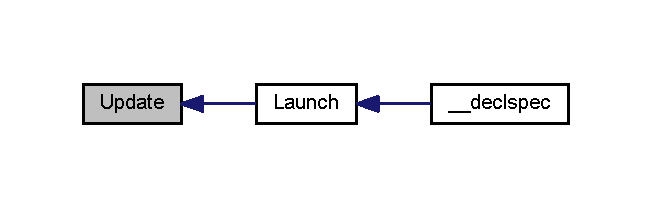
\includegraphics[width=313pt]{class_comet_engine_1_1_comet_engine_win32_a5ceefb272acf4d0adb4964ec29e5996e_icgraph}
\end{center}
\end{figure}


\subsection{멤버 데이터 문서화}
\mbox{\Hypertarget{class_comet_engine_1_1_comet_engine_win32_ac980c50873d6df828203b639e543de14}\label{class_comet_engine_1_1_comet_engine_win32_ac980c50873d6df828203b639e543de14}} 
\index{Comet\+Engine\+::\+Comet\+Engine\+Win32@{Comet\+Engine\+::\+Comet\+Engine\+Win32}!Instance@{Instance}}
\index{Instance@{Instance}!Comet\+Engine\+::\+Comet\+Engine\+Win32@{Comet\+Engine\+::\+Comet\+Engine\+Win32}}
\subsubsection{\texorpdfstring{Instance}{Instance}}
{\footnotesize\ttfamily \hyperlink{class_comet_engine_1_1_comet_engine_win32}{Comet\+Engine\+Win32} $\ast$ Instance = N\+U\+LL\hspace{0.3cm}{\ttfamily [static]}, {\ttfamily [private]}}



Comet\+Engine\+Win32.\+h 파일의 23 번째 라인에서 정의되었습니다.

\mbox{\Hypertarget{class_comet_engine_1_1_comet_engine_win32_ae5ce9d2610ee7e9675a4ecc74b0c9492}\label{class_comet_engine_1_1_comet_engine_win32_ae5ce9d2610ee7e9675a4ecc74b0c9492}} 
\index{Comet\+Engine\+::\+Comet\+Engine\+Win32@{Comet\+Engine\+::\+Comet\+Engine\+Win32}!m\+Height@{m\+Height}}
\index{m\+Height@{m\+Height}!Comet\+Engine\+::\+Comet\+Engine\+Win32@{Comet\+Engine\+::\+Comet\+Engine\+Win32}}
\subsubsection{\texorpdfstring{m\+Height}{mHeight}}
{\footnotesize\ttfamily U\+I\+NT m\+Height\hspace{0.3cm}{\ttfamily [private]}}



Comet\+Engine\+Win32.\+h 파일의 41 번째 라인에서 정의되었습니다.

\mbox{\Hypertarget{class_comet_engine_1_1_comet_engine_win32_a699a17c72a7b5416a8966df051f9c752}\label{class_comet_engine_1_1_comet_engine_win32_a699a17c72a7b5416a8966df051f9c752}} 
\index{Comet\+Engine\+::\+Comet\+Engine\+Win32@{Comet\+Engine\+::\+Comet\+Engine\+Win32}!mh\+Instance@{mh\+Instance}}
\index{mh\+Instance@{mh\+Instance}!Comet\+Engine\+::\+Comet\+Engine\+Win32@{Comet\+Engine\+::\+Comet\+Engine\+Win32}}
\subsubsection{\texorpdfstring{mh\+Instance}{mhInstance}}
{\footnotesize\ttfamily H\+I\+N\+S\+T\+A\+N\+CE mh\+Instance\hspace{0.3cm}{\ttfamily [private]}}



Comet\+Engine\+Win32.\+h 파일의 39 번째 라인에서 정의되었습니다.

\mbox{\Hypertarget{class_comet_engine_1_1_comet_engine_win32_a31c6576456c4bfea9672c5198aa18460}\label{class_comet_engine_1_1_comet_engine_win32_a31c6576456c4bfea9672c5198aa18460}} 
\index{Comet\+Engine\+::\+Comet\+Engine\+Win32@{Comet\+Engine\+::\+Comet\+Engine\+Win32}!m\+Hwnd@{m\+Hwnd}}
\index{m\+Hwnd@{m\+Hwnd}!Comet\+Engine\+::\+Comet\+Engine\+Win32@{Comet\+Engine\+::\+Comet\+Engine\+Win32}}
\subsubsection{\texorpdfstring{m\+Hwnd}{mHwnd}}
{\footnotesize\ttfamily H\+W\+ND m\+Hwnd\hspace{0.3cm}{\ttfamily [private]}}



Comet\+Engine\+Win32.\+h 파일의 38 번째 라인에서 정의되었습니다.

\mbox{\Hypertarget{class_comet_engine_1_1_comet_engine_win32_a954be7feb8f6558f86a08a30d640013e}\label{class_comet_engine_1_1_comet_engine_win32_a954be7feb8f6558f86a08a30d640013e}} 
\index{Comet\+Engine\+::\+Comet\+Engine\+Win32@{Comet\+Engine\+::\+Comet\+Engine\+Win32}!m\+Width@{m\+Width}}
\index{m\+Width@{m\+Width}!Comet\+Engine\+::\+Comet\+Engine\+Win32@{Comet\+Engine\+::\+Comet\+Engine\+Win32}}
\subsubsection{\texorpdfstring{m\+Width}{mWidth}}
{\footnotesize\ttfamily U\+I\+NT m\+Width\hspace{0.3cm}{\ttfamily [private]}}



Comet\+Engine\+Win32.\+h 파일의 40 번째 라인에서 정의되었습니다.

\mbox{\Hypertarget{class_comet_engine_1_1_comet_engine_win32_a31fa5cdc3ed0a81919f9ae7ec61844d1}\label{class_comet_engine_1_1_comet_engine_win32_a31fa5cdc3ed0a81919f9ae7ec61844d1}} 
\index{Comet\+Engine\+::\+Comet\+Engine\+Win32@{Comet\+Engine\+::\+Comet\+Engine\+Win32}!m\+Window\+Mode@{m\+Window\+Mode}}
\index{m\+Window\+Mode@{m\+Window\+Mode}!Comet\+Engine\+::\+Comet\+Engine\+Win32@{Comet\+Engine\+::\+Comet\+Engine\+Win32}}
\subsubsection{\texorpdfstring{m\+Window\+Mode}{mWindowMode}}
{\footnotesize\ttfamily \hyperlink{namespace_comet_engine_abdc5ec13bf1dfb1d26eb0bcc9da0ddad}{W\+I\+N\+D\+O\+W\+\_\+\+M\+O\+DE} m\+Window\+Mode\hspace{0.3cm}{\ttfamily [private]}}



Comet\+Engine\+Win32.\+h 파일의 43 번째 라인에서 정의되었습니다.

\mbox{\Hypertarget{class_comet_engine_1_1_comet_engine_win32_a63ee29dd5d917889a0e7b644fea26d06}\label{class_comet_engine_1_1_comet_engine_win32_a63ee29dd5d917889a0e7b644fea26d06}} 
\index{Comet\+Engine\+::\+Comet\+Engine\+Win32@{Comet\+Engine\+::\+Comet\+Engine\+Win32}!m\+Window\+Title@{m\+Window\+Title}}
\index{m\+Window\+Title@{m\+Window\+Title}!Comet\+Engine\+::\+Comet\+Engine\+Win32@{Comet\+Engine\+::\+Comet\+Engine\+Win32}}
\subsubsection{\texorpdfstring{m\+Window\+Title}{mWindowTitle}}
{\footnotesize\ttfamily wchar\+\_\+t$\ast$ m\+Window\+Title\hspace{0.3cm}{\ttfamily [private]}}



Comet\+Engine\+Win32.\+h 파일의 37 번째 라인에서 정의되었습니다.

\mbox{\Hypertarget{class_comet_engine_1_1_comet_engine_win32_a805efc6c9b43dd5daa64e3c1392d18b3}\label{class_comet_engine_1_1_comet_engine_win32_a805efc6c9b43dd5daa64e3c1392d18b3}} 
\index{Comet\+Engine\+::\+Comet\+Engine\+Win32@{Comet\+Engine\+::\+Comet\+Engine\+Win32}!Render@{Render}}
\index{Render@{Render}!Comet\+Engine\+::\+Comet\+Engine\+Win32@{Comet\+Engine\+::\+Comet\+Engine\+Win32}}
\subsubsection{\texorpdfstring{Render}{Render}}
{\footnotesize\ttfamily \hyperlink{class_comet_engine_1_1_comet_engine_win32_a97e4f6f1bfb397686ef973fe8bd42abf}{Render\+\_\+func} Render\hspace{0.3cm}{\ttfamily [private]}}



Comet\+Engine\+Win32.\+h 파일의 44 번째 라인에서 정의되었습니다.



이 클래스에 대한 문서화 페이지는 다음의 파일들로부터 생성되었습니다.\+:\begin{DoxyCompactItemize}
\item 
Comet\+Engine\+Client/\+Comet\+Engine\+Win32/\+Win32/\hyperlink{_comet_engine_win32_8h}{Comet\+Engine\+Win32.\+h}\item 
Comet\+Engine\+Client/\+Comet\+Engine\+Win32/\+Win32/\hyperlink{_comet_engine_win32_8cpp}{Comet\+Engine\+Win32.\+cpp}\end{DoxyCompactItemize}

\hypertarget{struct_comet_engine_1_1_core_1_1_memory_1_1_free_list_allocator_1_1_free_block_type}{}\section{Free\+List\+Allocator\+:\+:Free\+Block\+Type 구조체 참조}
\label{struct_comet_engine_1_1_core_1_1_memory_1_1_free_list_allocator_1_1_free_block_type}\index{Free\+List\+Allocator\+::\+Free\+Block\+Type@{Free\+List\+Allocator\+::\+Free\+Block\+Type}}


Free\+List\+Allocator\+:\+:Free\+Block\+Type에 대한 협력 다이어그램\+:\nopagebreak
\begin{figure}[H]
\begin{center}
\leavevmode
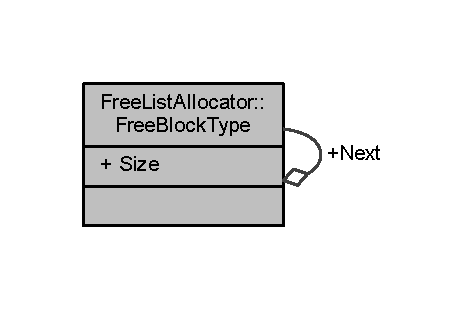
\includegraphics[width=224pt]{struct_comet_engine_1_1_core_1_1_memory_1_1_free_list_allocator_1_1_free_block_type__coll__graph}
\end{center}
\end{figure}
\subsection*{Public 속성}
\begin{DoxyCompactItemize}
\item 
\hyperlink{struct_comet_engine_1_1_core_1_1_memory_1_1_free_list_allocator_1_1_free_block_type}{Free\+Block\+Type} $\ast$ \hyperlink{struct_comet_engine_1_1_core_1_1_memory_1_1_free_list_allocator_1_1_free_block_type_a85617a85510a3465dbae6a061308aef7}{Next}
\item 
\hyperlink{namespace_comet_engine_1_1_type_a7c94ea6f8948649f8d181ae55911eeaf}{Type\+::size\+\_\+t} \hyperlink{struct_comet_engine_1_1_core_1_1_memory_1_1_free_list_allocator_1_1_free_block_type_ae6cf85bdf7b52a990d4428449e599c8e}{Size}
\end{DoxyCompactItemize}


\subsection{상세한 설명}


Comet\+Engine\+Memory.\+h 파일의 78 번째 라인에서 정의되었습니다.



\subsection{멤버 데이터 문서화}
\mbox{\Hypertarget{struct_comet_engine_1_1_core_1_1_memory_1_1_free_list_allocator_1_1_free_block_type_a85617a85510a3465dbae6a061308aef7}\label{struct_comet_engine_1_1_core_1_1_memory_1_1_free_list_allocator_1_1_free_block_type_a85617a85510a3465dbae6a061308aef7}} 
\index{Comet\+Engine\+::\+Core\+::\+Memory\+::\+Free\+List\+Allocator\+::\+Free\+Block\+Type@{Comet\+Engine\+::\+Core\+::\+Memory\+::\+Free\+List\+Allocator\+::\+Free\+Block\+Type}!Next@{Next}}
\index{Next@{Next}!Comet\+Engine\+::\+Core\+::\+Memory\+::\+Free\+List\+Allocator\+::\+Free\+Block\+Type@{Comet\+Engine\+::\+Core\+::\+Memory\+::\+Free\+List\+Allocator\+::\+Free\+Block\+Type}}
\subsubsection{\texorpdfstring{Next}{Next}}
{\footnotesize\ttfamily \hyperlink{struct_comet_engine_1_1_core_1_1_memory_1_1_free_list_allocator_1_1_free_block_type}{Free\+Block\+Type}$\ast$ Next}



Comet\+Engine\+Memory.\+h 파일의 80 번째 라인에서 정의되었습니다.

\mbox{\Hypertarget{struct_comet_engine_1_1_core_1_1_memory_1_1_free_list_allocator_1_1_free_block_type_ae6cf85bdf7b52a990d4428449e599c8e}\label{struct_comet_engine_1_1_core_1_1_memory_1_1_free_list_allocator_1_1_free_block_type_ae6cf85bdf7b52a990d4428449e599c8e}} 
\index{Comet\+Engine\+::\+Core\+::\+Memory\+::\+Free\+List\+Allocator\+::\+Free\+Block\+Type@{Comet\+Engine\+::\+Core\+::\+Memory\+::\+Free\+List\+Allocator\+::\+Free\+Block\+Type}!Size@{Size}}
\index{Size@{Size}!Comet\+Engine\+::\+Core\+::\+Memory\+::\+Free\+List\+Allocator\+::\+Free\+Block\+Type@{Comet\+Engine\+::\+Core\+::\+Memory\+::\+Free\+List\+Allocator\+::\+Free\+Block\+Type}}
\subsubsection{\texorpdfstring{Size}{Size}}
{\footnotesize\ttfamily \hyperlink{namespace_comet_engine_1_1_type_a7c94ea6f8948649f8d181ae55911eeaf}{Type\+::size\+\_\+t} Size}



Comet\+Engine\+Memory.\+h 파일의 81 번째 라인에서 정의되었습니다.



이 구조체에 대한 문서화 페이지는 다음의 파일로부터 생성되었습니다.\+:\begin{DoxyCompactItemize}
\item 
Comet\+Engine\+Common/\+Comet\+Engine/\+Comet\+Engine/\+Memory/\hyperlink{_comet_engine_memory_8h}{Comet\+Engine\+Memory.\+h}\end{DoxyCompactItemize}

\hypertarget{class_comet_engine_1_1_core_1_1_memory_1_1_free_list_allocator}{}\section{Free\+List\+Allocator 클래스 참조}
\label{class_comet_engine_1_1_core_1_1_memory_1_1_free_list_allocator}\index{Free\+List\+Allocator@{Free\+List\+Allocator}}


Free-\/\+List�� ������� �ϴ� Ŀ���� �޸� �Ҵ����̴�.  




{\ttfamily \#include $<$Comet\+Engine\+Memory.\+h$>$}



Free\+List\+Allocator에 대한 상속 다이어그램 \+: \nopagebreak
\begin{figure}[H]
\begin{center}
\leavevmode
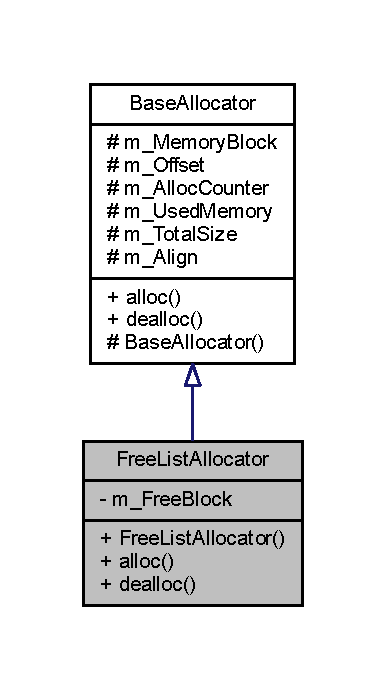
\includegraphics[width=185pt]{class_comet_engine_1_1_core_1_1_memory_1_1_free_list_allocator__inherit__graph}
\end{center}
\end{figure}


Free\+List\+Allocator에 대한 협력 다이어그램\+:\nopagebreak
\begin{figure}[H]
\begin{center}
\leavevmode
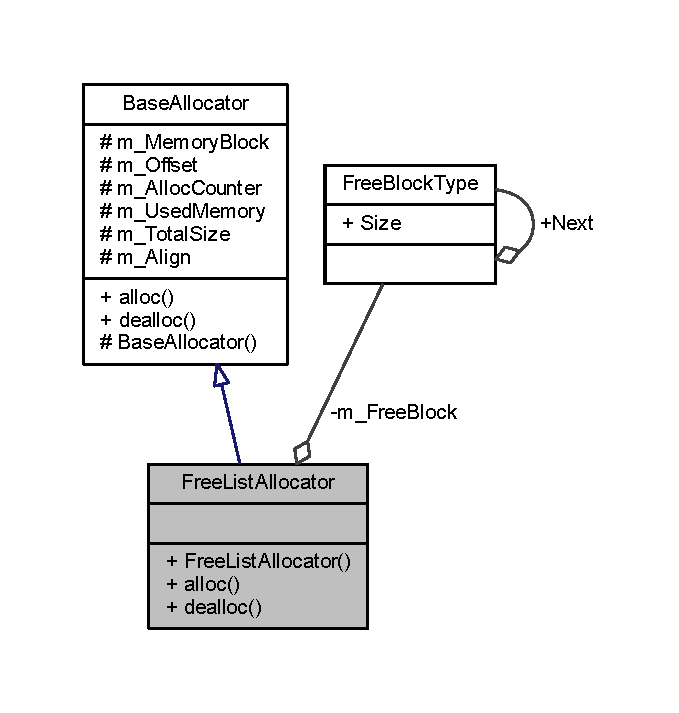
\includegraphics[width=326pt]{class_comet_engine_1_1_core_1_1_memory_1_1_free_list_allocator__coll__graph}
\end{center}
\end{figure}
\subsection*{클래스}
\begin{DoxyCompactItemize}
\item 
struct \hyperlink{struct_comet_engine_1_1_core_1_1_memory_1_1_free_list_allocator_1_1_free_block_type}{Free\+Block\+Type}
\item 
struct \hyperlink{struct_comet_engine_1_1_core_1_1_memory_1_1_free_list_allocator_1_1_memory_header}{Memory\+Header}
\end{DoxyCompactItemize}
\subsection*{Public 멤버 함수}
\begin{DoxyCompactItemize}
\item 
\hyperlink{class_comet_engine_1_1_core_1_1_memory_1_1_free_list_allocator_ae13641cb77ff097ec23c1a6112b2e6c6}{Free\+List\+Allocator} (void $\ast$i\+\_\+\+Memory\+Block, \hyperlink{namespace_comet_engine_1_1_type_a1b09856a6463f2bcc4bd8ff0e4e3ee0f}{Type\+::uint8} i\+\_\+align, \hyperlink{namespace_comet_engine_1_1_type_a7c94ea6f8948649f8d181ae55911eeaf}{Type\+::size\+\_\+t} i\+\_\+\+Memory\+Size, \hyperlink{namespace_comet_engine_1_1_type_a7c94ea6f8948649f8d181ae55911eeaf}{Type\+::size\+\_\+t} i\+\_\+offset=0)
\begin{DoxyCompactList}\small\item\em \hyperlink{class_comet_engine_1_1_core_1_1_memory_1_1_free_list_allocator}{Free\+List\+Allocator} ������. \end{DoxyCompactList}\item 
virtual void $\ast$ \hyperlink{class_comet_engine_1_1_core_1_1_memory_1_1_free_list_allocator_a73ff0a374ba86a2c447aaf05ad04e932}{alloc} (\hyperlink{namespace_comet_engine_1_1_type_a7c94ea6f8948649f8d181ae55911eeaf}{Type\+::size\+\_\+t} i\+\_\+byte) override
\begin{DoxyCompactList}\small\item\em i\+\_\+byte ��ŭ �޸𸮸� �Ҵ��մϴ�. \end{DoxyCompactList}\item 
virtual void \hyperlink{class_comet_engine_1_1_core_1_1_memory_1_1_free_list_allocator_ab7a97e4b1500c7ef2c2edc3bec28a84f}{dealloc} (void $\ast$i\+\_\+\+Adress) override
\begin{DoxyCompactList}\small\item\em i\+\_\+\+Adress�� ����Ű�� �ִ� �޸𸮸� �Ҵ� �����մϴ�. \end{DoxyCompactList}\end{DoxyCompactItemize}
\subsection*{Protected 속성}
\begin{DoxyCompactItemize}
\item 
void $\ast$ \hyperlink{class_comet_engine_1_1_core_1_1_memory_1_1_base_allocator_a24b4bdf45e7f4b6109b6d1cc455c6f26}{m\+\_\+\+Memory\+Block}
\item 
\hyperlink{namespace_comet_engine_1_1_type_a7c94ea6f8948649f8d181ae55911eeaf}{Type\+::size\+\_\+t} \hyperlink{class_comet_engine_1_1_core_1_1_memory_1_1_base_allocator_a71e2142fb28745ce9bc64de3a0ea1956}{m\+\_\+\+Offset}
\item 
\hyperlink{namespace_comet_engine_1_1_type_a7c94ea6f8948649f8d181ae55911eeaf}{Type\+::size\+\_\+t} \hyperlink{class_comet_engine_1_1_core_1_1_memory_1_1_base_allocator_abed7f06b465ee178701fe2cfc1aff9a6}{m\+\_\+\+Alloc\+Counter}
\item 
\hyperlink{namespace_comet_engine_1_1_type_a7c94ea6f8948649f8d181ae55911eeaf}{Type\+::size\+\_\+t} \hyperlink{class_comet_engine_1_1_core_1_1_memory_1_1_base_allocator_a1420047b91508f9ab33c448e8371511c}{m\+\_\+\+Used\+Memory}
\item 
\hyperlink{namespace_comet_engine_1_1_type_a7c94ea6f8948649f8d181ae55911eeaf}{Type\+::size\+\_\+t} \hyperlink{class_comet_engine_1_1_core_1_1_memory_1_1_base_allocator_abba9914681f05b98a55770daaf7d94be}{m\+\_\+\+Total\+Size}
\item 
\hyperlink{namespace_comet_engine_1_1_type_a1b09856a6463f2bcc4bd8ff0e4e3ee0f}{Type\+::uint8} \hyperlink{class_comet_engine_1_1_core_1_1_memory_1_1_base_allocator_a01f973630e3c1ac98b9defda193793b8}{m\+\_\+\+Align}
\end{DoxyCompactItemize}
\subsection*{Private 속성}
\begin{DoxyCompactItemize}
\item 
\hyperlink{struct_comet_engine_1_1_core_1_1_memory_1_1_free_list_allocator_1_1_free_block_type}{Free\+Block\+Type} $\ast$ \hyperlink{class_comet_engine_1_1_core_1_1_memory_1_1_free_list_allocator_a9e6f8b10d6e94738d154d9f7c72d2538}{m\+\_\+\+Free\+Block}
\end{DoxyCompactItemize}


\subsection{상세한 설명}
Free-\/\+List�� ������� �ϴ� Ŀ���� �޸� �Ҵ����̴�. 

�Ҵ�� �޸� ������ ������, Free-\/\+List�� �����Ͽ�, ���� ���� �޸� �Ҵ� ��ġ�� ã�� �Ҵ����ִ� ������ �Ѵ�.

\begin{DoxyAuthor}{작성자}
Dev S\+DK, \href{mailto:k_sdk@naver.com}{\tt k\+\_\+sdk@naver.\+com} 
\end{DoxyAuthor}
\begin{DoxyDate}{날짜}
2017-\/06-\/23 
\end{DoxyDate}
\begin{DoxyVersion}{버전}
0.\+0.\+1 
\end{DoxyVersion}


Comet\+Engine\+Memory.\+h 파일의 76 번째 라인에서 정의되었습니다.



\subsection{생성자 \& 소멸자 문서화}
\mbox{\Hypertarget{class_comet_engine_1_1_core_1_1_memory_1_1_free_list_allocator_ae13641cb77ff097ec23c1a6112b2e6c6}\label{class_comet_engine_1_1_core_1_1_memory_1_1_free_list_allocator_ae13641cb77ff097ec23c1a6112b2e6c6}} 
\index{Comet\+Engine\+::\+Core\+::\+Memory\+::\+Free\+List\+Allocator@{Comet\+Engine\+::\+Core\+::\+Memory\+::\+Free\+List\+Allocator}!Free\+List\+Allocator@{Free\+List\+Allocator}}
\index{Free\+List\+Allocator@{Free\+List\+Allocator}!Comet\+Engine\+::\+Core\+::\+Memory\+::\+Free\+List\+Allocator@{Comet\+Engine\+::\+Core\+::\+Memory\+::\+Free\+List\+Allocator}}
\subsubsection{\texorpdfstring{Free\+List\+Allocator()}{FreeListAllocator()}}
{\footnotesize\ttfamily \hyperlink{class_comet_engine_1_1_core_1_1_memory_1_1_free_list_allocator}{Free\+List\+Allocator} (\begin{DoxyParamCaption}\item[{void $\ast$}]{i\+\_\+\+Memory\+Block,  }\item[{\hyperlink{namespace_comet_engine_1_1_type_a1b09856a6463f2bcc4bd8ff0e4e3ee0f}{Type\+::uint8}}]{i\+\_\+align,  }\item[{\hyperlink{namespace_comet_engine_1_1_type_a7c94ea6f8948649f8d181ae55911eeaf}{Type\+::size\+\_\+t}}]{i\+\_\+\+Memory\+Size,  }\item[{\hyperlink{namespace_comet_engine_1_1_type_a7c94ea6f8948649f8d181ae55911eeaf}{Type\+::size\+\_\+t}}]{i\+\_\+offset = {\ttfamily 0} }\end{DoxyParamCaption})}



\hyperlink{class_comet_engine_1_1_core_1_1_memory_1_1_free_list_allocator}{Free\+List\+Allocator} ������. 


\begin{DoxyParams}{매개변수}
{\em void$\ast$} & i\+\_\+\+Memory\+Block ������ �޸� ������ �Է����� �޴´�. 16����Ʈ���� Ŀ���Ѵ�. \\
\hline
{\em \hyperlink{namespace_comet_engine_1_1_type_a1b09856a6463f2bcc4bd8ff0e4e3ee0f}{Type\+::uint8}} & i\+\_\+align �޸� ���� ũ�� \\
\hline
{\em \hyperlink{namespace_comet_engine_1_1_type_a7c94ea6f8948649f8d181ae55911eeaf}{Type\+::size\+\_\+t}} & i\+\_\+\+Memory\+Size ����� �޸��� ũ��. \\
\hline
{\em \hyperlink{namespace_comet_engine_1_1_type_a7c94ea6f8948649f8d181ae55911eeaf}{Type\+::size\+\_\+t}} & i\+\_\+offset �޸��� ���� ��ġ�� �˸��� offset default=0 \\
\hline
\end{DoxyParams}


Comet\+Engine\+Memory.\+cpp 파일의 54 번째 라인에서 정의되었습니다.


\begin{DoxyCode}
55     : \hyperlink{class_comet_engine_1_1_core_1_1_memory_1_1_base_allocator_a389c24863a5abee333f325634c18bea3}{BaseAllocator}(i\_MemoryBlock, i\_align, i\_MemorySize, i\_offset)
56 \{
57     \hyperlink{class_comet_engine_1_1_core_1_1_memory_1_1_free_list_allocator_a9e6f8b10d6e94738d154d9f7c72d2538}{m\_FreeBlock} = (FreeBlockType*)\hyperlink{class_comet_engine_1_1_core_1_1_memory_1_1_base_allocator_a24b4bdf45e7f4b6109b6d1cc455c6f26}{m\_MemoryBlock};
58     \hyperlink{class_comet_engine_1_1_core_1_1_memory_1_1_free_list_allocator_a9e6f8b10d6e94738d154d9f7c72d2538}{m\_FreeBlock}->\hyperlink{struct_comet_engine_1_1_core_1_1_memory_1_1_free_list_allocator_1_1_free_block_type_a85617a85510a3465dbae6a061308aef7}{Next} = \textcolor{keyword}{nullptr};
59     \hyperlink{class_comet_engine_1_1_core_1_1_memory_1_1_free_list_allocator_a9e6f8b10d6e94738d154d9f7c72d2538}{m\_FreeBlock}->\hyperlink{struct_comet_engine_1_1_core_1_1_memory_1_1_free_list_allocator_1_1_free_block_type_ae6cf85bdf7b52a990d4428449e599c8e}{Size} = \hyperlink{class_comet_engine_1_1_core_1_1_memory_1_1_base_allocator_abba9914681f05b98a55770daaf7d94be}{m\_TotalSize};
60 \}
\end{DoxyCode}


\subsection{멤버 함수 문서화}
\mbox{\Hypertarget{class_comet_engine_1_1_core_1_1_memory_1_1_free_list_allocator_a73ff0a374ba86a2c447aaf05ad04e932}\label{class_comet_engine_1_1_core_1_1_memory_1_1_free_list_allocator_a73ff0a374ba86a2c447aaf05ad04e932}} 
\index{Comet\+Engine\+::\+Core\+::\+Memory\+::\+Free\+List\+Allocator@{Comet\+Engine\+::\+Core\+::\+Memory\+::\+Free\+List\+Allocator}!alloc@{alloc}}
\index{alloc@{alloc}!Comet\+Engine\+::\+Core\+::\+Memory\+::\+Free\+List\+Allocator@{Comet\+Engine\+::\+Core\+::\+Memory\+::\+Free\+List\+Allocator}}
\subsubsection{\texorpdfstring{alloc()}{alloc()}}
{\footnotesize\ttfamily void $\ast$ alloc (\begin{DoxyParamCaption}\item[{\hyperlink{namespace_comet_engine_1_1_type_a7c94ea6f8948649f8d181ae55911eeaf}{Type\+::size\+\_\+t}}]{i\+\_\+byte }\end{DoxyParamCaption})\hspace{0.3cm}{\ttfamily [override]}, {\ttfamily [virtual]}}



i\+\_\+byte ��ŭ �޸𸮸� �Ҵ��մϴ�. 


\begin{DoxyParams}{매개변수}
{\em \hyperlink{namespace_comet_engine_1_1_type_a7c94ea6f8948649f8d181ae55911eeaf}{Type\+::size\+\_\+t}} & i\+\_\+byte �޸� �Ҵ� ũ�� \\
\hline
\end{DoxyParams}
\begin{DoxyReturn}{반환값}
�Ҵ�� �޸��� ���� �ּҸ� ��ȯ 
\end{DoxyReturn}


\hyperlink{class_comet_engine_1_1_core_1_1_memory_1_1_base_allocator_a8f51b4daa12e31477f57003494c09098}{Base\+Allocator}를 구현.



Comet\+Engine\+Memory.\+cpp 파일의 62 번째 라인에서 정의되었습니다.


\begin{DoxyCode}
63 \{
64     \textcolor{comment}{//Iteration �� �ʿ��� Node�� ����}
65     FreeBlockType* block = \hyperlink{class_comet_engine_1_1_core_1_1_memory_1_1_free_list_allocator_a9e6f8b10d6e94738d154d9f7c72d2538}{m\_FreeBlock};
66     FreeBlockType* preblock = \textcolor{keyword}{nullptr};
67 
68     \textcolor{comment}{//�������� ��ġ�� ã������ ����.}
69     \textcolor{comment}{//First-Fit Find Allocation Position}
70     \textcolor{keywordflow}{while} (block != \textcolor{keyword}{nullptr})
71     \{
72         \textcolor{comment}{//������ ������ ���� ����ũ��}
73         \hyperlink{namespace_comet_engine_1_1_type_a1b09856a6463f2bcc4bd8ff0e4e3ee0f}{Type::uint8} adjustment = \hyperlink{namespace_comet_engine_1_1_core_1_1_memory_1_1_utils_a57bbceefc56fa0e2ec1e472d85ce5e19}{Utils::alignForwardHeader}(block, 
      \hyperlink{class_comet_engine_1_1_core_1_1_memory_1_1_base_allocator_a01f973630e3c1ac98b9defda193793b8}{m\_Align}, \textcolor{keyword}{sizeof}(MemoryHeader));
74         \hyperlink{namespace_comet_engine_1_1_type_a7c94ea6f8948649f8d181ae55911eeaf}{Type::size\_t} request\_size = i\_size + adjustment;
75         
76         \textcolor{comment}{//�Ҵ��� �� �ִ� ������ ã�´�. (��������)}
77         \textcolor{keywordflow}{if} (block->Size < request\_size)
78         \{
79             preblock = block;
80             block = block->Next;
81             \textcolor{keywordflow}{continue};
82         \}
83         
84         \textcolor{comment}{//����ü�� Align�� �����ϰ� �ִ��� üũ.}
85         static\_assert(\textcolor{keyword}{sizeof}(MemoryHeader) >= \textcolor{keyword}{sizeof}(FreeBlockType), \textcolor{stringliteral}{"sizeof(AdjustmentHeader) >=
       sizeof(FreeBlockType)"});
86 
87 
88         \textcolor{comment}{//��û ���� ũ�Ⱑ, Ÿ��Ʈ �ϸ�}
89         \textcolor{keywordflow}{if} (block->Size - request\_size <= \textcolor{keyword}{sizeof}(MemoryHeader))
90         \{
91             \textcolor{comment}{//��ûũ�⸦ ������ ũ��� ������}
92             request\_size = block->Size;
93             \textcolor{keywordflow}{if} (preblock != \textcolor{keyword}{nullptr})
94                 preblock->Next = block->Next;
95             \textcolor{keywordflow}{else}
96                 \hyperlink{class_comet_engine_1_1_core_1_1_memory_1_1_free_list_allocator_a9e6f8b10d6e94738d154d9f7c72d2538}{m\_FreeBlock} = block->\hyperlink{struct_comet_engine_1_1_core_1_1_memory_1_1_free_list_allocator_1_1_free_block_type_a85617a85510a3465dbae6a061308aef7}{Next};
97         \}
98         \textcolor{keywordflow}{else}
99         \{
100             \textcolor{comment}{//����� ������ �ִٸ�,}
101             FreeBlockType* next = (FreeBlockType*)\hyperlink{namespace_comet_engine_1_1_core_1_1_memory_1_1_utils_a93ae170a43dac9da0116187242b35a6f}{Utils::Add}(block, (\textcolor{keywordtype}{void}*)request\_size);
102             \textcolor{comment}{//�޸� ������ �ڸ���}
103             next->Size = block->Size - request\_size;
104             \textcolor{comment}{//�� ������ ������ FreeList���� �����Ų��.}
105             next->Next = block->Next;
106 
107             \textcolor{keywordflow}{if} (preblock != \textcolor{keyword}{nullptr})
108                 preblock->Next = next;
109             \textcolor{keywordflow}{else}
110                 \hyperlink{class_comet_engine_1_1_core_1_1_memory_1_1_free_list_allocator_a9e6f8b10d6e94738d154d9f7c72d2538}{m\_FreeBlock} = next;
111         \}
112         \textcolor{comment}{//�ش��� �ְ�, ���ĵ� �ּҰ��� �����ϱ����� adjustment ���� �ִ´�.}
113         \hyperlink{namespace_comet_engine_1_1_type_aeb22ad46de677e9a50679dfebeb0e6f0}{Type::ptr} adress = (\hyperlink{namespace_comet_engine_1_1_type_aeb22ad46de677e9a50679dfebeb0e6f0}{Type::ptr})block + adjustment;
114         \textcolor{comment}{//�ش��� ����}
115         MemoryHeader* header = (MemoryHeader*)(adress - \textcolor{keyword}{sizeof}(MemoryHeader));
116         header->\hyperlink{struct_comet_engine_1_1_core_1_1_memory_1_1_free_list_allocator_1_1_free_block_type_ae6cf85bdf7b52a990d4428449e599c8e}{Size} = request\_size;
117         header->Adjustment = adjustment;
118         \hyperlink{class_comet_engine_1_1_core_1_1_memory_1_1_base_allocator_a1420047b91508f9ab33c448e8371511c}{m\_UsedMemory} += request\_size;
119         \hyperlink{class_comet_engine_1_1_core_1_1_memory_1_1_base_allocator_abed7f06b465ee178701fe2cfc1aff9a6}{m\_AllocCounter}++;
120 
121         \hyperlink{_comet_engine_types_8h_a9ade07b7881f4aeffa184676c123b87c}{CEAssert}(\hyperlink{namespace_comet_engine_1_1_core_1_1_memory_1_1_utils_aa5a0140d498d631a747be87791063f2d}{Utils::alignForwardAdjustment}((\textcolor{keywordtype}{void}*)adress, 
      \hyperlink{class_comet_engine_1_1_core_1_1_memory_1_1_base_allocator_a01f973630e3c1ac98b9defda193793b8}{m\_Align}) == 0);
122 
123         \textcolor{keywordflow}{return} (\textcolor{keywordtype}{void}*)adress;
124     \}
125 \textcolor{preprocessor}{#ifdef \_DEBUG}
126     \hyperlink{_comet_engine_types_8h_a9ade07b7881f4aeffa184676c123b87c}{CEAssert}(!\textcolor{stringliteral}{"Not eonugh memory block"});
127 \textcolor{preprocessor}{#endif}
128     \textcolor{keywordflow}{return} \textcolor{keyword}{nullptr};
129 \}
\end{DoxyCode}
이 함수 내부에서 호출하는 함수들에 대한 그래프입니다.\+:\nopagebreak
\begin{figure}[H]
\begin{center}
\leavevmode
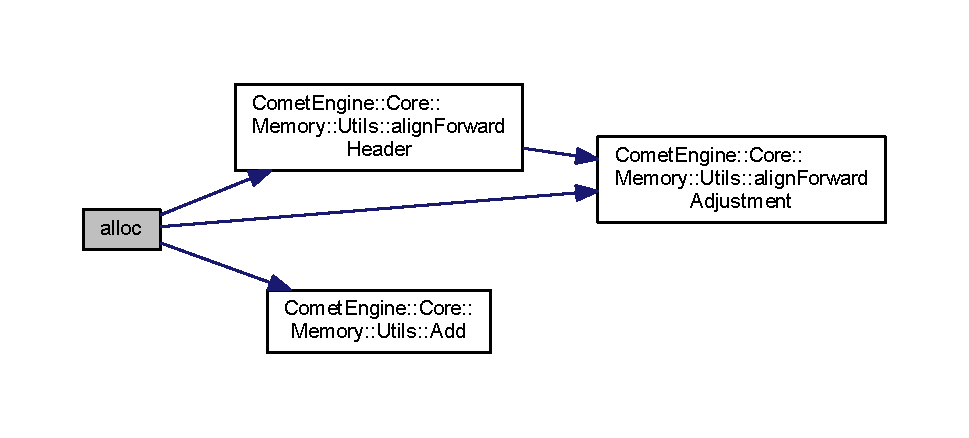
\includegraphics[width=350pt]{class_comet_engine_1_1_core_1_1_memory_1_1_free_list_allocator_a73ff0a374ba86a2c447aaf05ad04e932_cgraph}
\end{center}
\end{figure}
이 함수를 호출하는 함수들에 대한 그래프입니다.\+:\nopagebreak
\begin{figure}[H]
\begin{center}
\leavevmode
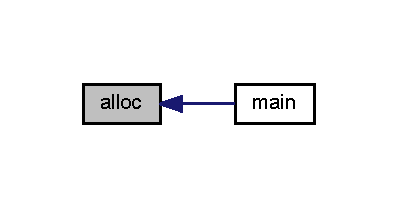
\includegraphics[width=191pt]{class_comet_engine_1_1_core_1_1_memory_1_1_free_list_allocator_a73ff0a374ba86a2c447aaf05ad04e932_icgraph}
\end{center}
\end{figure}
\mbox{\Hypertarget{class_comet_engine_1_1_core_1_1_memory_1_1_free_list_allocator_ab7a97e4b1500c7ef2c2edc3bec28a84f}\label{class_comet_engine_1_1_core_1_1_memory_1_1_free_list_allocator_ab7a97e4b1500c7ef2c2edc3bec28a84f}} 
\index{Comet\+Engine\+::\+Core\+::\+Memory\+::\+Free\+List\+Allocator@{Comet\+Engine\+::\+Core\+::\+Memory\+::\+Free\+List\+Allocator}!dealloc@{dealloc}}
\index{dealloc@{dealloc}!Comet\+Engine\+::\+Core\+::\+Memory\+::\+Free\+List\+Allocator@{Comet\+Engine\+::\+Core\+::\+Memory\+::\+Free\+List\+Allocator}}
\subsubsection{\texorpdfstring{dealloc()}{dealloc()}}
{\footnotesize\ttfamily void dealloc (\begin{DoxyParamCaption}\item[{void $\ast$}]{i\+\_\+\+Adress }\end{DoxyParamCaption})\hspace{0.3cm}{\ttfamily [override]}, {\ttfamily [virtual]}}



i\+\_\+\+Adress�� ����Ű�� �ִ� �޸𸮸� �Ҵ� �����մϴ�. 


\begin{DoxyParams}{매개변수}
{\em void$\ast$} & i\+\_\+\+Adress �Ҵ� ������ �޸� �ּ� \\
\hline
\end{DoxyParams}


\hyperlink{class_comet_engine_1_1_core_1_1_memory_1_1_base_allocator_acca0d1592319cfecb53f8333033a644b}{Base\+Allocator}를 구현.



Comet\+Engine\+Memory.\+cpp 파일의 131 번째 라인에서 정의되었습니다.


\begin{DoxyCode}
132 \{
133     \hyperlink{_comet_engine_types_8h_a9ade07b7881f4aeffa184676c123b87c}{CEAssert}(i\_Adress != \textcolor{keyword}{nullptr});
134     \textcolor{comment}{//�Ҵ��ߴ� �޸𸮿��� �ش����� ����}
135     MemoryHeader* header = (MemoryHeader*)\hyperlink{namespace_comet_engine_1_1_core_1_1_memory_1_1_utils_a4e360b8988f0de099daa987e3b5f09ed}{Utils::Sub}(i\_Adress, (\textcolor{keywordtype}{void}*)\textcolor{keyword}{sizeof}(MemoryHeader));
136 
137 
138     \textcolor{comment}{//�޸� ������ ���� ������}
139     \hyperlink{namespace_comet_engine_1_1_type_aeb22ad46de677e9a50679dfebeb0e6f0}{Type::ptr} block\_begin = ((\hyperlink{namespace_comet_engine_1_1_type_aeb22ad46de677e9a50679dfebeb0e6f0}{Type::ptr})i\_Adress) - header->Adjustment;
140     \hyperlink{namespace_comet_engine_1_1_type_a7c94ea6f8948649f8d181ae55911eeaf}{Type::size\_t} block\_size = header->Size;
141     \textcolor{comment}{//�޸� ������ �� ������}
142     \hyperlink{namespace_comet_engine_1_1_type_aeb22ad46de677e9a50679dfebeb0e6f0}{Type::ptr} block\_end = block\_begin + block\_size;
143 
144     \textcolor{comment}{//�ʱ�ȭ�� ������ Ȯ���ϱ� ���� 0����  �ʱ�ȭ}
145 \textcolor{preprocessor}{#ifdef \_DEBUG}
146     \textcolor{keywordflow}{for} (\hyperlink{namespace_comet_engine_1_1_type_aeb22ad46de677e9a50679dfebeb0e6f0}{Type::ptr} i = (\hyperlink{namespace_comet_engine_1_1_type_aeb22ad46de677e9a50679dfebeb0e6f0}{Type::ptr})i\_Adress; i != block\_end; i++)
147     \{
148         (*((\textcolor{keywordtype}{char}*)i)) = 0;
149     \}
150 \textcolor{preprocessor}{#endif}
151     FreeBlockType* block = \hyperlink{class_comet_engine_1_1_core_1_1_memory_1_1_free_list_allocator_a9e6f8b10d6e94738d154d9f7c72d2538}{m\_FreeBlock};
152     FreeBlockType* preblock = \textcolor{keyword}{nullptr};
153 
154     \textcolor{keywordflow}{while} (block != \textcolor{keyword}{nullptr})
155     \{
156         \textcolor{comment}{//���ĵ� ����Ʈ�� �����ϱ� ���� ��ġ Ž��}
157         \textcolor{keywordflow}{if} ((\hyperlink{namespace_comet_engine_1_1_type_aeb22ad46de677e9a50679dfebeb0e6f0}{Type::ptr})block >= block\_end)
158             \textcolor{keywordflow}{break};
159         preblock = block;
160         block = block->\hyperlink{struct_comet_engine_1_1_core_1_1_memory_1_1_free_list_allocator_1_1_free_block_type_a85617a85510a3465dbae6a061308aef7}{Next};
161     \}
162 
163     \textcolor{keywordflow}{if} (preblock == \textcolor{keyword}{nullptr})
164     \{
165         \textcolor{comment}{//���� ������ ���� ���¶�� }
166         \textcolor{comment}{//���� ������ ���� ������ ������ ����Ű�� �ѵ� ���������� ������������ �ٲ�.( �׳� �ڿ��ΰ� ����)}
167         preblock = (FreeBlockType*)block\_begin;
168         preblock->\hyperlink{struct_comet_engine_1_1_core_1_1_memory_1_1_free_list_allocator_1_1_free_block_type_ae6cf85bdf7b52a990d4428449e599c8e}{Size} = block\_size;
169         preblock->Next = \hyperlink{class_comet_engine_1_1_core_1_1_memory_1_1_free_list_allocator_a9e6f8b10d6e94738d154d9f7c72d2538}{m\_FreeBlock};
170         \hyperlink{class_comet_engine_1_1_core_1_1_memory_1_1_free_list_allocator_a9e6f8b10d6e94738d154d9f7c72d2538}{m\_FreeBlock} = preblock;
171     \}
172     \textcolor{keywordflow}{else} \textcolor{keywordflow}{if} ((\hyperlink{namespace_comet_engine_1_1_type_aeb22ad46de677e9a50679dfebeb0e6f0}{Type::ptr}) preblock + preblock->Size == block\_begin)
173     \{
174         \textcolor{comment}{//�� ������ �ٷ� ���������� ���������� �ִٸ�, ������ ����� Ű��.}
175         preblock->\hyperlink{struct_comet_engine_1_1_core_1_1_memory_1_1_free_list_allocator_1_1_free_block_type_ae6cf85bdf7b52a990d4428449e599c8e}{Size} += block\_size;
176     \}
177     \textcolor{keywordflow}{else}
178     \{
179         \textcolor{comment}{//���� ��带 ����}
180         FreeBlockType* freeblock = (FreeBlockType*)block\_begin;
181         freeblock->Size = block\_size;
182         \textcolor{comment}{//��� �߰��� ��������. preblock->freeblock-> preblock�� ����Ű�� ���}
183         freeblock->Next = preblock->Next;
184         preblock->Next = freeblock;
185         preblock = freeblock;
186     \}
187 
188     \textcolor{comment}{//�������� ��尡 ���� ������, �� ��带 ������}
189     \textcolor{keywordflow}{if} (block != \textcolor{keyword}{nullptr} && (\hyperlink{namespace_comet_engine_1_1_type_aeb22ad46de677e9a50679dfebeb0e6f0}{Type::ptr})block == block\_end)
190     \{
191         preblock->Size += block->Size;
192         preblock->Next = block->Next;
193     \}
194 
195     \hyperlink{class_comet_engine_1_1_core_1_1_memory_1_1_base_allocator_abed7f06b465ee178701fe2cfc1aff9a6}{m\_AllocCounter}--;
196     \hyperlink{class_comet_engine_1_1_core_1_1_memory_1_1_base_allocator_a1420047b91508f9ab33c448e8371511c}{m\_UsedMemory} -= block\_size;
197 
198 \}
\end{DoxyCode}
이 함수 내부에서 호출하는 함수들에 대한 그래프입니다.\+:\nopagebreak
\begin{figure}[H]
\begin{center}
\leavevmode
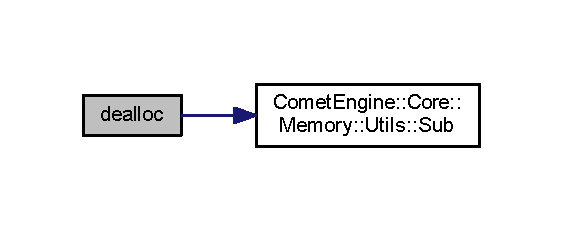
\includegraphics[width=270pt]{class_comet_engine_1_1_core_1_1_memory_1_1_free_list_allocator_ab7a97e4b1500c7ef2c2edc3bec28a84f_cgraph}
\end{center}
\end{figure}
이 함수를 호출하는 함수들에 대한 그래프입니다.\+:\nopagebreak
\begin{figure}[H]
\begin{center}
\leavevmode
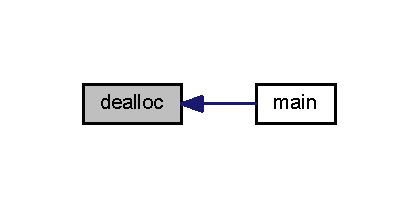
\includegraphics[width=201pt]{class_comet_engine_1_1_core_1_1_memory_1_1_free_list_allocator_ab7a97e4b1500c7ef2c2edc3bec28a84f_icgraph}
\end{center}
\end{figure}


\subsection{멤버 데이터 문서화}
\mbox{\Hypertarget{class_comet_engine_1_1_core_1_1_memory_1_1_base_allocator_a01f973630e3c1ac98b9defda193793b8}\label{class_comet_engine_1_1_core_1_1_memory_1_1_base_allocator_a01f973630e3c1ac98b9defda193793b8}} 
\index{Comet\+Engine\+::\+Core\+::\+Memory\+::\+Free\+List\+Allocator@{Comet\+Engine\+::\+Core\+::\+Memory\+::\+Free\+List\+Allocator}!m\+\_\+\+Align@{m\+\_\+\+Align}}
\index{m\+\_\+\+Align@{m\+\_\+\+Align}!Comet\+Engine\+::\+Core\+::\+Memory\+::\+Free\+List\+Allocator@{Comet\+Engine\+::\+Core\+::\+Memory\+::\+Free\+List\+Allocator}}
\subsubsection{\texorpdfstring{m\+\_\+\+Align}{m\_Align}}
{\footnotesize\ttfamily \hyperlink{namespace_comet_engine_1_1_type_a1b09856a6463f2bcc4bd8ff0e4e3ee0f}{Type\+::uint8} m\+\_\+\+Align\hspace{0.3cm}{\ttfamily [protected]}, {\ttfamily [inherited]}}



Comet\+Engine\+Memory.\+h 파일의 59 번째 라인에서 정의되었습니다.

\mbox{\Hypertarget{class_comet_engine_1_1_core_1_1_memory_1_1_base_allocator_abed7f06b465ee178701fe2cfc1aff9a6}\label{class_comet_engine_1_1_core_1_1_memory_1_1_base_allocator_abed7f06b465ee178701fe2cfc1aff9a6}} 
\index{Comet\+Engine\+::\+Core\+::\+Memory\+::\+Free\+List\+Allocator@{Comet\+Engine\+::\+Core\+::\+Memory\+::\+Free\+List\+Allocator}!m\+\_\+\+Alloc\+Counter@{m\+\_\+\+Alloc\+Counter}}
\index{m\+\_\+\+Alloc\+Counter@{m\+\_\+\+Alloc\+Counter}!Comet\+Engine\+::\+Core\+::\+Memory\+::\+Free\+List\+Allocator@{Comet\+Engine\+::\+Core\+::\+Memory\+::\+Free\+List\+Allocator}}
\subsubsection{\texorpdfstring{m\+\_\+\+Alloc\+Counter}{m\_AllocCounter}}
{\footnotesize\ttfamily \hyperlink{namespace_comet_engine_1_1_type_a7c94ea6f8948649f8d181ae55911eeaf}{Type\+::size\+\_\+t} m\+\_\+\+Alloc\+Counter\hspace{0.3cm}{\ttfamily [protected]}, {\ttfamily [inherited]}}



Comet\+Engine\+Memory.\+h 파일의 56 번째 라인에서 정의되었습니다.

\mbox{\Hypertarget{class_comet_engine_1_1_core_1_1_memory_1_1_free_list_allocator_a9e6f8b10d6e94738d154d9f7c72d2538}\label{class_comet_engine_1_1_core_1_1_memory_1_1_free_list_allocator_a9e6f8b10d6e94738d154d9f7c72d2538}} 
\index{Comet\+Engine\+::\+Core\+::\+Memory\+::\+Free\+List\+Allocator@{Comet\+Engine\+::\+Core\+::\+Memory\+::\+Free\+List\+Allocator}!m\+\_\+\+Free\+Block@{m\+\_\+\+Free\+Block}}
\index{m\+\_\+\+Free\+Block@{m\+\_\+\+Free\+Block}!Comet\+Engine\+::\+Core\+::\+Memory\+::\+Free\+List\+Allocator@{Comet\+Engine\+::\+Core\+::\+Memory\+::\+Free\+List\+Allocator}}
\subsubsection{\texorpdfstring{m\+\_\+\+Free\+Block}{m\_FreeBlock}}
{\footnotesize\ttfamily \hyperlink{struct_comet_engine_1_1_core_1_1_memory_1_1_free_list_allocator_1_1_free_block_type}{Free\+Block\+Type}$\ast$ m\+\_\+\+Free\+Block\hspace{0.3cm}{\ttfamily [private]}}



Comet\+Engine\+Memory.\+h 파일의 90 번째 라인에서 정의되었습니다.

\mbox{\Hypertarget{class_comet_engine_1_1_core_1_1_memory_1_1_base_allocator_a24b4bdf45e7f4b6109b6d1cc455c6f26}\label{class_comet_engine_1_1_core_1_1_memory_1_1_base_allocator_a24b4bdf45e7f4b6109b6d1cc455c6f26}} 
\index{Comet\+Engine\+::\+Core\+::\+Memory\+::\+Free\+List\+Allocator@{Comet\+Engine\+::\+Core\+::\+Memory\+::\+Free\+List\+Allocator}!m\+\_\+\+Memory\+Block@{m\+\_\+\+Memory\+Block}}
\index{m\+\_\+\+Memory\+Block@{m\+\_\+\+Memory\+Block}!Comet\+Engine\+::\+Core\+::\+Memory\+::\+Free\+List\+Allocator@{Comet\+Engine\+::\+Core\+::\+Memory\+::\+Free\+List\+Allocator}}
\subsubsection{\texorpdfstring{m\+\_\+\+Memory\+Block}{m\_MemoryBlock}}
{\footnotesize\ttfamily void$\ast$ m\+\_\+\+Memory\+Block\hspace{0.3cm}{\ttfamily [protected]}, {\ttfamily [inherited]}}



Comet\+Engine\+Memory.\+h 파일의 54 번째 라인에서 정의되었습니다.

\mbox{\Hypertarget{class_comet_engine_1_1_core_1_1_memory_1_1_base_allocator_a71e2142fb28745ce9bc64de3a0ea1956}\label{class_comet_engine_1_1_core_1_1_memory_1_1_base_allocator_a71e2142fb28745ce9bc64de3a0ea1956}} 
\index{Comet\+Engine\+::\+Core\+::\+Memory\+::\+Free\+List\+Allocator@{Comet\+Engine\+::\+Core\+::\+Memory\+::\+Free\+List\+Allocator}!m\+\_\+\+Offset@{m\+\_\+\+Offset}}
\index{m\+\_\+\+Offset@{m\+\_\+\+Offset}!Comet\+Engine\+::\+Core\+::\+Memory\+::\+Free\+List\+Allocator@{Comet\+Engine\+::\+Core\+::\+Memory\+::\+Free\+List\+Allocator}}
\subsubsection{\texorpdfstring{m\+\_\+\+Offset}{m\_Offset}}
{\footnotesize\ttfamily \hyperlink{namespace_comet_engine_1_1_type_a7c94ea6f8948649f8d181ae55911eeaf}{Type\+::size\+\_\+t} m\+\_\+\+Offset\hspace{0.3cm}{\ttfamily [protected]}, {\ttfamily [inherited]}}



Comet\+Engine\+Memory.\+h 파일의 55 번째 라인에서 정의되었습니다.

\mbox{\Hypertarget{class_comet_engine_1_1_core_1_1_memory_1_1_base_allocator_abba9914681f05b98a55770daaf7d94be}\label{class_comet_engine_1_1_core_1_1_memory_1_1_base_allocator_abba9914681f05b98a55770daaf7d94be}} 
\index{Comet\+Engine\+::\+Core\+::\+Memory\+::\+Free\+List\+Allocator@{Comet\+Engine\+::\+Core\+::\+Memory\+::\+Free\+List\+Allocator}!m\+\_\+\+Total\+Size@{m\+\_\+\+Total\+Size}}
\index{m\+\_\+\+Total\+Size@{m\+\_\+\+Total\+Size}!Comet\+Engine\+::\+Core\+::\+Memory\+::\+Free\+List\+Allocator@{Comet\+Engine\+::\+Core\+::\+Memory\+::\+Free\+List\+Allocator}}
\subsubsection{\texorpdfstring{m\+\_\+\+Total\+Size}{m\_TotalSize}}
{\footnotesize\ttfamily \hyperlink{namespace_comet_engine_1_1_type_a7c94ea6f8948649f8d181ae55911eeaf}{Type\+::size\+\_\+t} m\+\_\+\+Total\+Size\hspace{0.3cm}{\ttfamily [protected]}, {\ttfamily [inherited]}}



Comet\+Engine\+Memory.\+h 파일의 58 번째 라인에서 정의되었습니다.

\mbox{\Hypertarget{class_comet_engine_1_1_core_1_1_memory_1_1_base_allocator_a1420047b91508f9ab33c448e8371511c}\label{class_comet_engine_1_1_core_1_1_memory_1_1_base_allocator_a1420047b91508f9ab33c448e8371511c}} 
\index{Comet\+Engine\+::\+Core\+::\+Memory\+::\+Free\+List\+Allocator@{Comet\+Engine\+::\+Core\+::\+Memory\+::\+Free\+List\+Allocator}!m\+\_\+\+Used\+Memory@{m\+\_\+\+Used\+Memory}}
\index{m\+\_\+\+Used\+Memory@{m\+\_\+\+Used\+Memory}!Comet\+Engine\+::\+Core\+::\+Memory\+::\+Free\+List\+Allocator@{Comet\+Engine\+::\+Core\+::\+Memory\+::\+Free\+List\+Allocator}}
\subsubsection{\texorpdfstring{m\+\_\+\+Used\+Memory}{m\_UsedMemory}}
{\footnotesize\ttfamily \hyperlink{namespace_comet_engine_1_1_type_a7c94ea6f8948649f8d181ae55911eeaf}{Type\+::size\+\_\+t} m\+\_\+\+Used\+Memory\hspace{0.3cm}{\ttfamily [protected]}, {\ttfamily [inherited]}}



Comet\+Engine\+Memory.\+h 파일의 57 번째 라인에서 정의되었습니다.



이 클래스에 대한 문서화 페이지는 다음의 파일들로부터 생성되었습니다.\+:\begin{DoxyCompactItemize}
\item 
Comet\+Engine\+Common/\+Comet\+Engine/\+Comet\+Engine/\+Memory/\hyperlink{_comet_engine_memory_8h}{Comet\+Engine\+Memory.\+h}\item 
Comet\+Engine\+Common/\+Comet\+Engine/\+Comet\+Engine/\+Memory/\hyperlink{_comet_engine_memory_8cpp}{Comet\+Engine\+Memory.\+cpp}\end{DoxyCompactItemize}

\hypertarget{struct_comet_engine_1_1_core_1_1_memory_1_1_free_list_allocator_1_1_memory_header}{}\section{Free\+List\+Allocator\+:\+:Memory\+Header 구조체 참조}
\label{struct_comet_engine_1_1_core_1_1_memory_1_1_free_list_allocator_1_1_memory_header}\index{Free\+List\+Allocator\+::\+Memory\+Header@{Free\+List\+Allocator\+::\+Memory\+Header}}


Free\+List\+Allocator\+:\+:Memory\+Header에 대한 협력 다이어그램\+:\nopagebreak
\begin{figure}[H]
\begin{center}
\leavevmode
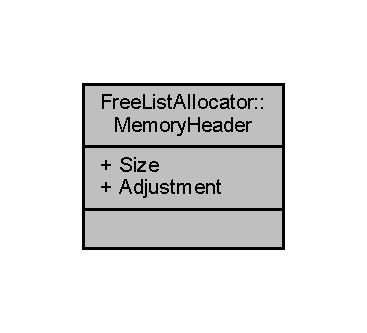
\includegraphics[width=176pt]{struct_comet_engine_1_1_core_1_1_memory_1_1_free_list_allocator_1_1_memory_header__coll__graph}
\end{center}
\end{figure}
\subsection*{Public 속성}
\begin{DoxyCompactItemize}
\item 
\hyperlink{namespace_comet_engine_1_1_type_a7c94ea6f8948649f8d181ae55911eeaf}{Type\+::size\+\_\+t} \hyperlink{struct_comet_engine_1_1_core_1_1_memory_1_1_free_list_allocator_1_1_memory_header_ae6cf85bdf7b52a990d4428449e599c8e}{Size}
\item 
\hyperlink{namespace_comet_engine_1_1_type_a1b09856a6463f2bcc4bd8ff0e4e3ee0f}{Type\+::uint8} \hyperlink{struct_comet_engine_1_1_core_1_1_memory_1_1_free_list_allocator_1_1_memory_header_ad3a03b9a927b866d54e19f7558846c6a}{Adjustment}
\end{DoxyCompactItemize}


\subsection{상세한 설명}


Comet\+Engine\+Memory.\+h 파일의 84 번째 라인에서 정의되었습니다.



\subsection{멤버 데이터 문서화}
\mbox{\Hypertarget{struct_comet_engine_1_1_core_1_1_memory_1_1_free_list_allocator_1_1_memory_header_ad3a03b9a927b866d54e19f7558846c6a}\label{struct_comet_engine_1_1_core_1_1_memory_1_1_free_list_allocator_1_1_memory_header_ad3a03b9a927b866d54e19f7558846c6a}} 
\index{Comet\+Engine\+::\+Core\+::\+Memory\+::\+Free\+List\+Allocator\+::\+Memory\+Header@{Comet\+Engine\+::\+Core\+::\+Memory\+::\+Free\+List\+Allocator\+::\+Memory\+Header}!Adjustment@{Adjustment}}
\index{Adjustment@{Adjustment}!Comet\+Engine\+::\+Core\+::\+Memory\+::\+Free\+List\+Allocator\+::\+Memory\+Header@{Comet\+Engine\+::\+Core\+::\+Memory\+::\+Free\+List\+Allocator\+::\+Memory\+Header}}
\subsubsection{\texorpdfstring{Adjustment}{Adjustment}}
{\footnotesize\ttfamily \hyperlink{namespace_comet_engine_1_1_type_a1b09856a6463f2bcc4bd8ff0e4e3ee0f}{Type\+::uint8} Adjustment}



Comet\+Engine\+Memory.\+h 파일의 87 번째 라인에서 정의되었습니다.

\mbox{\Hypertarget{struct_comet_engine_1_1_core_1_1_memory_1_1_free_list_allocator_1_1_memory_header_ae6cf85bdf7b52a990d4428449e599c8e}\label{struct_comet_engine_1_1_core_1_1_memory_1_1_free_list_allocator_1_1_memory_header_ae6cf85bdf7b52a990d4428449e599c8e}} 
\index{Comet\+Engine\+::\+Core\+::\+Memory\+::\+Free\+List\+Allocator\+::\+Memory\+Header@{Comet\+Engine\+::\+Core\+::\+Memory\+::\+Free\+List\+Allocator\+::\+Memory\+Header}!Size@{Size}}
\index{Size@{Size}!Comet\+Engine\+::\+Core\+::\+Memory\+::\+Free\+List\+Allocator\+::\+Memory\+Header@{Comet\+Engine\+::\+Core\+::\+Memory\+::\+Free\+List\+Allocator\+::\+Memory\+Header}}
\subsubsection{\texorpdfstring{Size}{Size}}
{\footnotesize\ttfamily \hyperlink{namespace_comet_engine_1_1_type_a7c94ea6f8948649f8d181ae55911eeaf}{Type\+::size\+\_\+t} Size}



Comet\+Engine\+Memory.\+h 파일의 86 번째 라인에서 정의되었습니다.



이 구조체에 대한 문서화 페이지는 다음의 파일로부터 생성되었습니다.\+:\begin{DoxyCompactItemize}
\item 
Comet\+Engine\+Common/\+Comet\+Engine/\+Comet\+Engine/\+Memory/\hyperlink{_comet_engine_memory_8h}{Comet\+Engine\+Memory.\+h}\end{DoxyCompactItemize}

\hypertarget{class_comet_engine_tester_1_1_program}{}\section{Program 클래스 참조}
\label{class_comet_engine_tester_1_1_program}\index{Program@{Program}}


Program에 대한 협력 다이어그램\+:\nopagebreak
\begin{figure}[H]
\begin{center}
\leavevmode
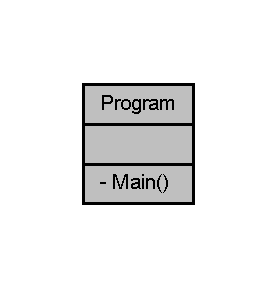
\includegraphics[width=133pt]{class_comet_engine_tester_1_1_program__coll__graph}
\end{center}
\end{figure}
\subsection*{정적 Private 멤버 함수}
\begin{DoxyCompactItemize}
\item 
static void \hyperlink{class_comet_engine_tester_1_1_program_a25f94f55e8993781b6a82d5eb88ea252}{Main} (string\mbox{[}$\,$\mbox{]} args)
\end{DoxyCompactItemize}


\subsection{상세한 설명}


Program.\+cs 파일의 9 번째 라인에서 정의되었습니다.



\subsection{멤버 함수 문서화}
\mbox{\Hypertarget{class_comet_engine_tester_1_1_program_a25f94f55e8993781b6a82d5eb88ea252}\label{class_comet_engine_tester_1_1_program_a25f94f55e8993781b6a82d5eb88ea252}} 
\index{Comet\+Engine\+Tester\+::\+Program@{Comet\+Engine\+Tester\+::\+Program}!Main@{Main}}
\index{Main@{Main}!Comet\+Engine\+Tester\+::\+Program@{Comet\+Engine\+Tester\+::\+Program}}
\subsubsection{\texorpdfstring{Main()}{Main()}}
{\footnotesize\ttfamily static void Main (\begin{DoxyParamCaption}\item[{string \mbox{[}$\,$\mbox{]}}]{args }\end{DoxyParamCaption})\hspace{0.3cm}{\ttfamily [inline]}, {\ttfamily [static]}, {\ttfamily [private]}}



Program.\+cs 파일의 11 번째 라인에서 정의되었습니다.


\begin{DoxyCode}
12         \{
13             \hyperlink{class_comet_engine_1_1_client_1_1_comet_engine_client}{CometEngineClient}.\hyperlink{class_comet_engine_1_1_client_1_1_comet_engine_client_af5f8db49a5de5bb41cf935066d21f5aa}{Init}(\textcolor{stringliteral}{"TITLE"}, 1200, 600, 
      \hyperlink{namespace_comet_engine_1_1_client_a608d2e459fd95babca189e50f4182a65}{WIndowModes}.DEFAULT, 1, 1);
14             
15 
16             \textcolor{comment}{// TODO: Init Renderer }
17 
18 
19 
20 
21             \hyperlink{class_comet_engine_1_1_client_1_1_comet_engine_client}{CometEngineClient}.\hyperlink{class_comet_engine_1_1_client_1_1_comet_engine_client_aee7b13887a71ba1fcd42c5fbccf124d4}{Launch}();
22 
23 
24         \}
\end{DoxyCode}
이 함수 내부에서 호출하는 함수들에 대한 그래프입니다.\+:\nopagebreak
\begin{figure}[H]
\begin{center}
\leavevmode
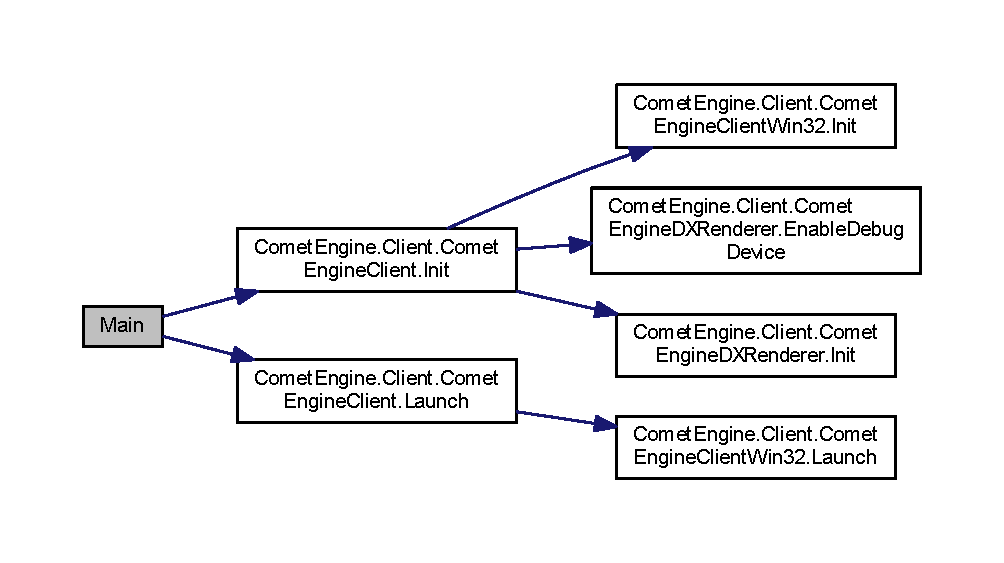
\includegraphics[width=350pt]{class_comet_engine_tester_1_1_program_a25f94f55e8993781b6a82d5eb88ea252_cgraph}
\end{center}
\end{figure}


이 클래스에 대한 문서화 페이지는 다음의 파일로부터 생성되었습니다.\+:\begin{DoxyCompactItemize}
\item 
Comet\+Engine\+Tester/\hyperlink{_program_8cs}{Program.\+cs}\end{DoxyCompactItemize}

\chapter{파일 문서화}
\hypertarget{_d_l_l_comet_engine_renderer_8cpp}{}\section{Comet\+Engine\+Client/\+Comet\+Engine\+Renderer/\+D\+L\+L\+Export/\+D\+L\+L\+Comet\+Engine\+Renderer.cpp 파일 참조}
\label{_d_l_l_comet_engine_renderer_8cpp}\index{Comet\+Engine\+Client/\+Comet\+Engine\+Renderer/\+D\+L\+L\+Export/\+D\+L\+L\+Comet\+Engine\+Renderer.\+cpp@{Comet\+Engine\+Client/\+Comet\+Engine\+Renderer/\+D\+L\+L\+Export/\+D\+L\+L\+Comet\+Engine\+Renderer.\+cpp}}
{\ttfamily \#include $<$Windows.\+h$>$}\newline
{\ttfamily \#include $<$string$>$}\newline
{\ttfamily \#include \char`\"{}../\+Renderer/\+Comet\+Engine\+D\+X\+Renderer.\+h\char`\"{}}\newline
D\+L\+L\+Comet\+Engine\+Renderer.\+cpp에 대한 include 의존 그래프\nopagebreak
\begin{figure}[H]
\begin{center}
\leavevmode
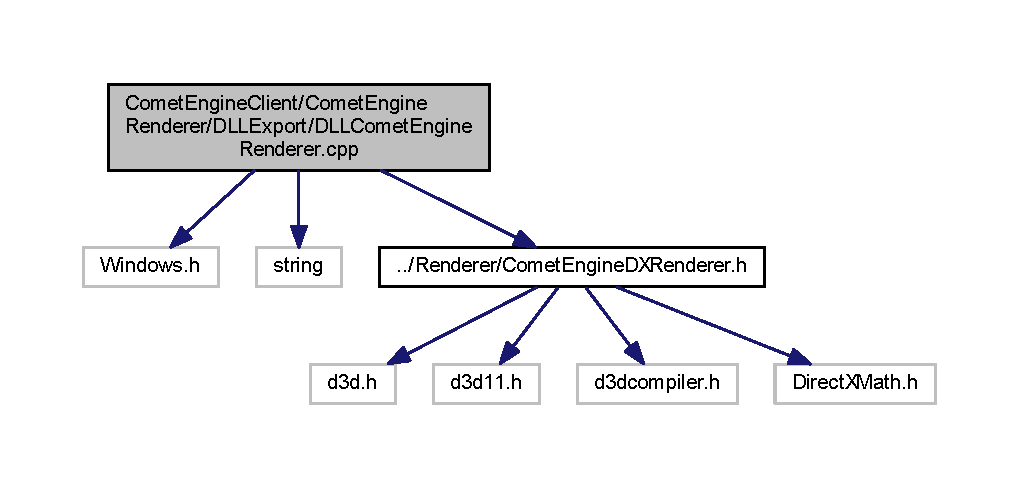
\includegraphics[width=350pt]{_d_l_l_comet_engine_renderer_8cpp__incl}
\end{center}
\end{figure}
\subsection*{함수}
\begin{DoxyCompactItemize}
\item 
\hyperlink{_d_l_l_comet_engine_renderer_8cpp_a56c623259192e033c4afcd528a148b57}{\+\_\+\+\_\+declspec} (dllexport) bool \+\_\+\+\_\+stdcall Init(int i\+\_\+\+Render\+Width
\end{DoxyCompactItemize}
\subsection*{변수}
\begin{DoxyCompactItemize}
\item 
int \hyperlink{_d_l_l_comet_engine_renderer_8cpp_ab996e2b2e12adfc087c67cebde9194e6}{i\+\_\+\+Render\+Height}
\item 
int int \hyperlink{_d_l_l_comet_engine_renderer_8cpp_a901222d6138bd4efc54d4eda8460c65b}{i\+\_\+\+Render\+Scale}
\item 
int int int \hyperlink{_d_l_l_comet_engine_renderer_8cpp_a7016fffcce13da83a94427468f9bf950}{i\+\_\+\+M\+S\+A\+A\+Scale}
\item 
int int int bool \hyperlink{_d_l_l_comet_engine_renderer_8cpp_aef2be053839ec77e7c50bd4f4997cef1}{i\+\_\+\+Is\+Full\+Screen}
\end{DoxyCompactItemize}


\subsection{함수 문서화}
\mbox{\Hypertarget{_d_l_l_comet_engine_renderer_8cpp_a56c623259192e033c4afcd528a148b57}\label{_d_l_l_comet_engine_renderer_8cpp_a56c623259192e033c4afcd528a148b57}} 
\index{D\+L\+L\+Comet\+Engine\+Renderer.\+cpp@{D\+L\+L\+Comet\+Engine\+Renderer.\+cpp}!\+\_\+\+\_\+declspec@{\+\_\+\+\_\+declspec}}
\index{\+\_\+\+\_\+declspec@{\+\_\+\+\_\+declspec}!D\+L\+L\+Comet\+Engine\+Renderer.\+cpp@{D\+L\+L\+Comet\+Engine\+Renderer.\+cpp}}
\subsubsection{\texorpdfstring{\+\_\+\+\_\+declspec()}{\_\_declspec()}}
{\footnotesize\ttfamily \+\_\+\+\_\+declspec (\begin{DoxyParamCaption}\item[{dllexport}]{ }\end{DoxyParamCaption})}



D\+L\+L\+Comet\+Engine\+Renderer.\+cpp 파일의 12 번째 라인에서 정의되었습니다.


\begin{DoxyCode}
13 \{
14     CometEngineDXRenderer::GetInstance()->Render(dt);
15 \}
\end{DoxyCode}
이 함수 내부에서 호출하는 함수들에 대한 그래프입니다.\+:\nopagebreak
\begin{figure}[H]
\begin{center}
\leavevmode
\includegraphics[width=350pt]{_d_l_l_comet_engine_renderer_8cpp_a56c623259192e033c4afcd528a148b57_cgraph}
\end{center}
\end{figure}


\subsection{변수 문서화}
\mbox{\Hypertarget{_d_l_l_comet_engine_renderer_8cpp_aef2be053839ec77e7c50bd4f4997cef1}\label{_d_l_l_comet_engine_renderer_8cpp_aef2be053839ec77e7c50bd4f4997cef1}} 
\index{D\+L\+L\+Comet\+Engine\+Renderer.\+cpp@{D\+L\+L\+Comet\+Engine\+Renderer.\+cpp}!i\+\_\+\+Is\+Full\+Screen@{i\+\_\+\+Is\+Full\+Screen}}
\index{i\+\_\+\+Is\+Full\+Screen@{i\+\_\+\+Is\+Full\+Screen}!D\+L\+L\+Comet\+Engine\+Renderer.\+cpp@{D\+L\+L\+Comet\+Engine\+Renderer.\+cpp}}
\subsubsection{\texorpdfstring{i\+\_\+\+Is\+Full\+Screen}{i\_IsFullScreen}}
{\footnotesize\ttfamily int int int bool i\+\_\+\+Is\+Full\+Screen}

{\bfseries 초기값\+:}
\begin{DoxyCode}
\{
    \textcolor{keywordflow}{return} CometEngineDXRenderer::GetInstance()->Init(i\_RenderWidth, 
      \hyperlink{_d_l_l_comet_engine_renderer_8cpp_ab996e2b2e12adfc087c67cebde9194e6}{i\_RenderHeight}, \hyperlink{_d_l_l_comet_engine_renderer_8cpp_a901222d6138bd4efc54d4eda8460c65b}{i\_RenderScale}, \hyperlink{_d_l_l_comet_engine_renderer_8cpp_a901222d6138bd4efc54d4eda8460c65b}{i\_RenderScale}, 
      \hyperlink{_d_l_l_comet_engine_renderer_8cpp_aef2be053839ec77e7c50bd4f4997cef1}{i\_IsFullScreen})
\end{DoxyCode}


D\+L\+L\+Comet\+Engine\+Renderer.\+cpp 파일의 8 번째 라인에서 정의되었습니다.

\mbox{\Hypertarget{_d_l_l_comet_engine_renderer_8cpp_a7016fffcce13da83a94427468f9bf950}\label{_d_l_l_comet_engine_renderer_8cpp_a7016fffcce13da83a94427468f9bf950}} 
\index{D\+L\+L\+Comet\+Engine\+Renderer.\+cpp@{D\+L\+L\+Comet\+Engine\+Renderer.\+cpp}!i\+\_\+\+M\+S\+A\+A\+Scale@{i\+\_\+\+M\+S\+A\+A\+Scale}}
\index{i\+\_\+\+M\+S\+A\+A\+Scale@{i\+\_\+\+M\+S\+A\+A\+Scale}!D\+L\+L\+Comet\+Engine\+Renderer.\+cpp@{D\+L\+L\+Comet\+Engine\+Renderer.\+cpp}}
\subsubsection{\texorpdfstring{i\+\_\+\+M\+S\+A\+A\+Scale}{i\_MSAAScale}}
{\footnotesize\ttfamily int int int i\+\_\+\+M\+S\+A\+A\+Scale}



D\+L\+L\+Comet\+Engine\+Renderer.\+cpp 파일의 7 번째 라인에서 정의되었습니다.

\mbox{\Hypertarget{_d_l_l_comet_engine_renderer_8cpp_ab996e2b2e12adfc087c67cebde9194e6}\label{_d_l_l_comet_engine_renderer_8cpp_ab996e2b2e12adfc087c67cebde9194e6}} 
\index{D\+L\+L\+Comet\+Engine\+Renderer.\+cpp@{D\+L\+L\+Comet\+Engine\+Renderer.\+cpp}!i\+\_\+\+Render\+Height@{i\+\_\+\+Render\+Height}}
\index{i\+\_\+\+Render\+Height@{i\+\_\+\+Render\+Height}!D\+L\+L\+Comet\+Engine\+Renderer.\+cpp@{D\+L\+L\+Comet\+Engine\+Renderer.\+cpp}}
\subsubsection{\texorpdfstring{i\+\_\+\+Render\+Height}{i\_RenderHeight}}
{\footnotesize\ttfamily int i\+\_\+\+Render\+Height}



D\+L\+L\+Comet\+Engine\+Renderer.\+cpp 파일의 7 번째 라인에서 정의되었습니다.

\mbox{\Hypertarget{_d_l_l_comet_engine_renderer_8cpp_a901222d6138bd4efc54d4eda8460c65b}\label{_d_l_l_comet_engine_renderer_8cpp_a901222d6138bd4efc54d4eda8460c65b}} 
\index{D\+L\+L\+Comet\+Engine\+Renderer.\+cpp@{D\+L\+L\+Comet\+Engine\+Renderer.\+cpp}!i\+\_\+\+Render\+Scale@{i\+\_\+\+Render\+Scale}}
\index{i\+\_\+\+Render\+Scale@{i\+\_\+\+Render\+Scale}!D\+L\+L\+Comet\+Engine\+Renderer.\+cpp@{D\+L\+L\+Comet\+Engine\+Renderer.\+cpp}}
\subsubsection{\texorpdfstring{i\+\_\+\+Render\+Scale}{i\_RenderScale}}
{\footnotesize\ttfamily int int i\+\_\+\+Render\+Scale}



D\+L\+L\+Comet\+Engine\+Renderer.\+cpp 파일의 7 번째 라인에서 정의되었습니다.


\hypertarget{_comet_engine_d_x_renderer_8cpp}{}\section{Comet\+Engine\+Client/\+Comet\+Engine\+Renderer/\+Renderer/\+Comet\+Engine\+D\+X\+Renderer.cpp 파일 참조}
\label{_comet_engine_d_x_renderer_8cpp}\index{Comet\+Engine\+Client/\+Comet\+Engine\+Renderer/\+Renderer/\+Comet\+Engine\+D\+X\+Renderer.\+cpp@{Comet\+Engine\+Client/\+Comet\+Engine\+Renderer/\+Renderer/\+Comet\+Engine\+D\+X\+Renderer.\+cpp}}
{\ttfamily \#include \char`\"{}Comet\+Engine\+D\+X\+Renderer.\+h\char`\"{}}\newline
{\ttfamily \#include $<$Direct\+X\+Colors.\+h$>$}\newline
{\ttfamily \#include $<$string$>$}\newline
Comet\+Engine\+D\+X\+Renderer.\+cpp에 대한 include 의존 그래프\nopagebreak
\begin{figure}[H]
\begin{center}
\leavevmode
\includegraphics[width=350pt]{_comet_engine_d_x_renderer_8cpp__incl}
\end{center}
\end{figure}
\subsection*{매크로}
\begin{DoxyCompactItemize}
\item 
\#define \hyperlink{_comet_engine_d_x_renderer_8cpp_a924cd8cbf81756869040aed04fd33ca5}{HR}(x)~\{ H\+R\+E\+S\+U\+LT n\+Value = (x); if(F\+A\+I\+L\+ED(n\+Value)) return false; \}
\end{DoxyCompactItemize}


\subsection{매크로 문서화}
\mbox{\Hypertarget{_comet_engine_d_x_renderer_8cpp_a924cd8cbf81756869040aed04fd33ca5}\label{_comet_engine_d_x_renderer_8cpp_a924cd8cbf81756869040aed04fd33ca5}} 
\index{Comet\+Engine\+D\+X\+Renderer.\+cpp@{Comet\+Engine\+D\+X\+Renderer.\+cpp}!HR@{HR}}
\index{HR@{HR}!Comet\+Engine\+D\+X\+Renderer.\+cpp@{Comet\+Engine\+D\+X\+Renderer.\+cpp}}
\subsubsection{\texorpdfstring{HR}{HR}}
{\footnotesize\ttfamily \#define HR(\begin{DoxyParamCaption}\item[{}]{x }\end{DoxyParamCaption})~\{ H\+R\+E\+S\+U\+LT n\+Value = (x); if(F\+A\+I\+L\+ED(n\+Value)) return false; \}}



Comet\+Engine\+D\+X\+Renderer.\+cpp 파일의 7 번째 라인에서 정의되었습니다.


\hypertarget{_comet_engine_d_x_renderer_8h}{}\section{Comet\+Engine\+Client/\+Comet\+Engine\+Renderer/\+Renderer/\+Comet\+Engine\+D\+X\+Renderer.h 파일 참조}
\label{_comet_engine_d_x_renderer_8h}\index{Comet\+Engine\+Client/\+Comet\+Engine\+Renderer/\+Renderer/\+Comet\+Engine\+D\+X\+Renderer.\+h@{Comet\+Engine\+Client/\+Comet\+Engine\+Renderer/\+Renderer/\+Comet\+Engine\+D\+X\+Renderer.\+h}}
{\ttfamily \#include $<$d3d.\+h$>$}\newline
{\ttfamily \#include $<$d3d11.\+h$>$}\newline
{\ttfamily \#include $<$d3dcompiler.\+h$>$}\newline
{\ttfamily \#include $<$Direct\+X\+Math.\+h$>$}\newline
Comet\+Engine\+D\+X\+Renderer.\+h에 대한 include 의존 그래프\nopagebreak
\begin{figure}[H]
\begin{center}
\leavevmode
\includegraphics[width=350pt]{_comet_engine_d_x_renderer_8h__incl}
\end{center}
\end{figure}
이 그래프는 이 파일을 직/간접적으로 include 하는 파일들을 보여줍니다.\+:\nopagebreak
\begin{figure}[H]
\begin{center}
\leavevmode
\includegraphics[width=350pt]{_comet_engine_d_x_renderer_8h__dep__incl}
\end{center}
\end{figure}
\subsection*{클래스}
\begin{DoxyCompactItemize}
\item 
class \hyperlink{class_comet_engine_1_1_renderer_1_1_comet_engine_d_x_renderer}{Comet\+Engine\+D\+X\+Renderer}
\end{DoxyCompactItemize}
\subsection*{네임스페이스}
\begin{DoxyCompactItemize}
\item 
 \hyperlink{namespace_comet_engine}{Comet\+Engine}
\item 
 \hyperlink{namespace_comet_engine_1_1_renderer}{Comet\+Engine\+::\+Renderer}
\end{DoxyCompactItemize}

\hypertarget{_d_l_l_comet_engine_win32_8cpp}{}\section{Comet\+Engine\+Client/\+Comet\+Engine\+Win32/\+D\+L\+L\+Export/\+D\+L\+L\+Comet\+Engine\+Win32.cpp 파일 참조}
\label{_d_l_l_comet_engine_win32_8cpp}\index{Comet\+Engine\+Client/\+Comet\+Engine\+Win32/\+D\+L\+L\+Export/\+D\+L\+L\+Comet\+Engine\+Win32.\+cpp@{Comet\+Engine\+Client/\+Comet\+Engine\+Win32/\+D\+L\+L\+Export/\+D\+L\+L\+Comet\+Engine\+Win32.\+cpp}}
{\ttfamily \#include $<$Windows.\+h$>$}\newline
{\ttfamily \#include $<$string$>$}\newline
{\ttfamily \#include \char`\"{}../\+Win32/\+Comet\+Engine\+Win32.\+h\char`\"{}}\newline
D\+L\+L\+Comet\+Engine\+Win32.\+cpp에 대한 include 의존 그래프\nopagebreak
\begin{figure}[H]
\begin{center}
\leavevmode
\includegraphics[width=313pt]{_d_l_l_comet_engine_win32_8cpp__incl}
\end{center}
\end{figure}
\subsection*{함수}
\begin{DoxyCompactItemize}
\item 
\hyperlink{_d_l_l_comet_engine_win32_8cpp_a2879621abf424abe46badd790ed99724}{\+\_\+\+\_\+declspec} (dllexport) bool \+\_\+\+\_\+stdcall Init(wchar\+\_\+t $\ast$Title
\end{DoxyCompactItemize}
\subsection*{변수}
\begin{DoxyCompactItemize}
\item 
int \hyperlink{_d_l_l_comet_engine_win32_8cpp_abbe7749c3b402f7dfe64f936774cfcd4}{Width}
\item 
int int \hyperlink{_d_l_l_comet_engine_win32_8cpp_afd53bc431b967813e00ae3cfecd5c548}{Height}
\item 
int int int \hyperlink{_d_l_l_comet_engine_win32_8cpp_a319b6c977f6b5f638f8246c67a367768}{Window\+Mode}
\item 
int int int H\+I\+N\+S\+T\+A\+N\+CE \hyperlink{_d_l_l_comet_engine_win32_8cpp_a5fb685beb2aed3ecdbad03b352111398}{h\+Instance}
\item 
int int int H\+I\+N\+S\+T\+A\+N\+CE L\+P\+S\+TR \hyperlink{_d_l_l_comet_engine_win32_8cpp_af1ff5ad877f6069d41720b03c7769227}{lp\+Cmd\+Line}
\end{DoxyCompactItemize}


\subsection{함수 문서화}
\mbox{\Hypertarget{_d_l_l_comet_engine_win32_8cpp_a2879621abf424abe46badd790ed99724}\label{_d_l_l_comet_engine_win32_8cpp_a2879621abf424abe46badd790ed99724}} 
\index{D\+L\+L\+Comet\+Engine\+Win32.\+cpp@{D\+L\+L\+Comet\+Engine\+Win32.\+cpp}!\+\_\+\+\_\+declspec@{\+\_\+\+\_\+declspec}}
\index{\+\_\+\+\_\+declspec@{\+\_\+\+\_\+declspec}!D\+L\+L\+Comet\+Engine\+Win32.\+cpp@{D\+L\+L\+Comet\+Engine\+Win32.\+cpp}}
\subsubsection{\texorpdfstring{\+\_\+\+\_\+declspec()}{\_\_declspec()}}
{\footnotesize\ttfamily \+\_\+\+\_\+declspec (\begin{DoxyParamCaption}\item[{dllexport}]{ }\end{DoxyParamCaption})}



D\+L\+L\+Comet\+Engine\+Win32.\+cpp 파일의 13 번째 라인에서 정의되었습니다.


\begin{DoxyCode}
14 \{
15     CometEngineWin32::GetInstance()->Launch();  
16 \}
\end{DoxyCode}
이 함수 내부에서 호출하는 함수들에 대한 그래프입니다.\+:\nopagebreak
\begin{figure}[H]
\begin{center}
\leavevmode
\includegraphics[width=350pt]{_d_l_l_comet_engine_win32_8cpp_a2879621abf424abe46badd790ed99724_cgraph}
\end{center}
\end{figure}


\subsection{변수 문서화}
\mbox{\Hypertarget{_d_l_l_comet_engine_win32_8cpp_afd53bc431b967813e00ae3cfecd5c548}\label{_d_l_l_comet_engine_win32_8cpp_afd53bc431b967813e00ae3cfecd5c548}} 
\index{D\+L\+L\+Comet\+Engine\+Win32.\+cpp@{D\+L\+L\+Comet\+Engine\+Win32.\+cpp}!Height@{Height}}
\index{Height@{Height}!D\+L\+L\+Comet\+Engine\+Win32.\+cpp@{D\+L\+L\+Comet\+Engine\+Win32.\+cpp}}
\subsubsection{\texorpdfstring{Height}{Height}}
{\footnotesize\ttfamily int int Height}



D\+L\+L\+Comet\+Engine\+Win32.\+cpp 파일의 8 번째 라인에서 정의되었습니다.

\mbox{\Hypertarget{_d_l_l_comet_engine_win32_8cpp_a5fb685beb2aed3ecdbad03b352111398}\label{_d_l_l_comet_engine_win32_8cpp_a5fb685beb2aed3ecdbad03b352111398}} 
\index{D\+L\+L\+Comet\+Engine\+Win32.\+cpp@{D\+L\+L\+Comet\+Engine\+Win32.\+cpp}!h\+Instance@{h\+Instance}}
\index{h\+Instance@{h\+Instance}!D\+L\+L\+Comet\+Engine\+Win32.\+cpp@{D\+L\+L\+Comet\+Engine\+Win32.\+cpp}}
\subsubsection{\texorpdfstring{h\+Instance}{hInstance}}
{\footnotesize\ttfamily int int int H\+I\+N\+S\+T\+A\+N\+CE h\+Instance}



D\+L\+L\+Comet\+Engine\+Win32.\+cpp 파일의 8 번째 라인에서 정의되었습니다.

\mbox{\Hypertarget{_d_l_l_comet_engine_win32_8cpp_af1ff5ad877f6069d41720b03c7769227}\label{_d_l_l_comet_engine_win32_8cpp_af1ff5ad877f6069d41720b03c7769227}} 
\index{D\+L\+L\+Comet\+Engine\+Win32.\+cpp@{D\+L\+L\+Comet\+Engine\+Win32.\+cpp}!lp\+Cmd\+Line@{lp\+Cmd\+Line}}
\index{lp\+Cmd\+Line@{lp\+Cmd\+Line}!D\+L\+L\+Comet\+Engine\+Win32.\+cpp@{D\+L\+L\+Comet\+Engine\+Win32.\+cpp}}
\subsubsection{\texorpdfstring{lp\+Cmd\+Line}{lpCmdLine}}
{\footnotesize\ttfamily int int int H\+I\+N\+S\+T\+A\+N\+CE L\+P\+S\+TR lp\+Cmd\+Line}

{\bfseries 초기값\+:}
\begin{DoxyCode}
\{
    \textcolor{keywordflow}{return} CometEngineWin32::GetInstance()->Init(Title,\hyperlink{_d_l_l_comet_engine_win32_8cpp_abbe7749c3b402f7dfe64f936774cfcd4}{Width},\hyperlink{_d_l_l_comet_engine_win32_8cpp_afd53bc431b967813e00ae3cfecd5c548}{Height}, (
      \hyperlink{namespace_comet_engine_abdc5ec13bf1dfb1d26eb0bcc9da0ddad}{WINDOW\_MODE})\hyperlink{_d_l_l_comet_engine_win32_8cpp_a319b6c977f6b5f638f8246c67a367768}{WindowMode}, \hyperlink{_d_l_l_comet_engine_win32_8cpp_a5fb685beb2aed3ecdbad03b352111398}{hInstance}, \hyperlink{_d_l_l_comet_engine_win32_8cpp_af1ff5ad877f6069d41720b03c7769227}{lpCmdLine})
\end{DoxyCode}


D\+L\+L\+Comet\+Engine\+Win32.\+cpp 파일의 9 번째 라인에서 정의되었습니다.

\mbox{\Hypertarget{_d_l_l_comet_engine_win32_8cpp_abbe7749c3b402f7dfe64f936774cfcd4}\label{_d_l_l_comet_engine_win32_8cpp_abbe7749c3b402f7dfe64f936774cfcd4}} 
\index{D\+L\+L\+Comet\+Engine\+Win32.\+cpp@{D\+L\+L\+Comet\+Engine\+Win32.\+cpp}!Width@{Width}}
\index{Width@{Width}!D\+L\+L\+Comet\+Engine\+Win32.\+cpp@{D\+L\+L\+Comet\+Engine\+Win32.\+cpp}}
\subsubsection{\texorpdfstring{Width}{Width}}
{\footnotesize\ttfamily int Width}



D\+L\+L\+Comet\+Engine\+Win32.\+cpp 파일의 8 번째 라인에서 정의되었습니다.

\mbox{\Hypertarget{_d_l_l_comet_engine_win32_8cpp_a319b6c977f6b5f638f8246c67a367768}\label{_d_l_l_comet_engine_win32_8cpp_a319b6c977f6b5f638f8246c67a367768}} 
\index{D\+L\+L\+Comet\+Engine\+Win32.\+cpp@{D\+L\+L\+Comet\+Engine\+Win32.\+cpp}!Window\+Mode@{Window\+Mode}}
\index{Window\+Mode@{Window\+Mode}!D\+L\+L\+Comet\+Engine\+Win32.\+cpp@{D\+L\+L\+Comet\+Engine\+Win32.\+cpp}}
\subsubsection{\texorpdfstring{Window\+Mode}{WindowMode}}
{\footnotesize\ttfamily int int int Window\+Mode}



D\+L\+L\+Comet\+Engine\+Win32.\+cpp 파일의 8 번째 라인에서 정의되었습니다.


\hypertarget{_comet_engine_win32_8cpp}{}\section{Comet\+Engine\+Client/\+Comet\+Engine\+Win32/\+Win32/\+Comet\+Engine\+Win32.cpp 파일 참조}
\label{_comet_engine_win32_8cpp}\index{Comet\+Engine\+Client/\+Comet\+Engine\+Win32/\+Win32/\+Comet\+Engine\+Win32.\+cpp@{Comet\+Engine\+Client/\+Comet\+Engine\+Win32/\+Win32/\+Comet\+Engine\+Win32.\+cpp}}
{\ttfamily \#include \char`\"{}Comet\+Engine\+Win32.\+h\char`\"{}}\newline
{\ttfamily \#include $<$string$>$}\newline
Comet\+Engine\+Win32.\+cpp에 대한 include 의존 그래프\nopagebreak
\begin{figure}[H]
\begin{center}
\leavevmode
\includegraphics[width=318pt]{_comet_engine_win32_8cpp__incl}
\end{center}
\end{figure}
\subsection*{매크로}
\begin{DoxyCompactItemize}
\item 
\#define \hyperlink{_comet_engine_win32_8cpp_a09ecca53f2cd1b8d1c566bedb245e141}{U\+N\+I\+C\+O\+DE}
\end{DoxyCompactItemize}


\subsection{매크로 문서화}
\mbox{\Hypertarget{_comet_engine_win32_8cpp_a09ecca53f2cd1b8d1c566bedb245e141}\label{_comet_engine_win32_8cpp_a09ecca53f2cd1b8d1c566bedb245e141}} 
\index{Comet\+Engine\+Win32.\+cpp@{Comet\+Engine\+Win32.\+cpp}!U\+N\+I\+C\+O\+DE@{U\+N\+I\+C\+O\+DE}}
\index{U\+N\+I\+C\+O\+DE@{U\+N\+I\+C\+O\+DE}!Comet\+Engine\+Win32.\+cpp@{Comet\+Engine\+Win32.\+cpp}}
\subsubsection{\texorpdfstring{U\+N\+I\+C\+O\+DE}{UNICODE}}
{\footnotesize\ttfamily \#define U\+N\+I\+C\+O\+DE}



Comet\+Engine\+Win32.\+cpp 파일의 1 번째 라인에서 정의되었습니다.


\hypertarget{_comet_engine_win32_8h}{}\section{Comet\+Engine\+Client/\+Comet\+Engine\+Win32/\+Win32/\+Comet\+Engine\+Win32.h 파일 참조}
\label{_comet_engine_win32_8h}\index{Comet\+Engine\+Client/\+Comet\+Engine\+Win32/\+Win32/\+Comet\+Engine\+Win32.\+h@{Comet\+Engine\+Client/\+Comet\+Engine\+Win32/\+Win32/\+Comet\+Engine\+Win32.\+h}}
{\ttfamily \#include $<$Windows.\+h$>$}\newline
{\ttfamily \#include $<$string$>$}\newline
{\ttfamily \#include $<$assert.\+h$>$}\newline
Comet\+Engine\+Win32.\+h에 대한 include 의존 그래프\nopagebreak
\begin{figure}[H]
\begin{center}
\leavevmode
\includegraphics[width=275pt]{_comet_engine_win32_8h__incl}
\end{center}
\end{figure}
이 그래프는 이 파일을 직/간접적으로 include 하는 파일들을 보여줍니다.\+:\nopagebreak
\begin{figure}[H]
\begin{center}
\leavevmode
\includegraphics[width=350pt]{_comet_engine_win32_8h__dep__incl}
\end{center}
\end{figure}
\subsection*{클래스}
\begin{DoxyCompactItemize}
\item 
class \hyperlink{class_comet_engine_1_1_comet_engine_win32}{Comet\+Engine\+Win32}
\end{DoxyCompactItemize}
\subsection*{네임스페이스}
\begin{DoxyCompactItemize}
\item 
 \hyperlink{namespace_comet_engine}{Comet\+Engine}
\end{DoxyCompactItemize}
\subsection*{열거형 타입}
\begin{DoxyCompactItemize}
\item 
enum \hyperlink{namespace_comet_engine_abdc5ec13bf1dfb1d26eb0bcc9da0ddad}{W\+I\+N\+D\+O\+W\+\_\+\+M\+O\+DE} \{ \hyperlink{namespace_comet_engine_abdc5ec13bf1dfb1d26eb0bcc9da0ddada88ec7d5086d2469ba843c7fcceade8a6}{D\+E\+F\+A\+U\+LT} = 0, 
\hyperlink{namespace_comet_engine_abdc5ec13bf1dfb1d26eb0bcc9da0ddada2fcf3c9ce3f39ff118fc4e667c4e2cc6}{N\+O\+\_\+\+B\+O\+R\+D\+ER}, 
\hyperlink{namespace_comet_engine_abdc5ec13bf1dfb1d26eb0bcc9da0ddada5f039f23ee85ddea038ca1ab88ca6755}{F\+U\+L\+L\+S\+C\+R\+E\+EN}
 \}
\end{DoxyCompactItemize}

\hypertarget{_comet_engine_client_8cs}{}\section{Comet\+Engine\+Client/\+I\+Comet\+Engine\+Client/\+Comet\+Engine\+Client.cs 파일 참조}
\label{_comet_engine_client_8cs}\index{Comet\+Engine\+Client/\+I\+Comet\+Engine\+Client/\+Comet\+Engine\+Client.\+cs@{Comet\+Engine\+Client/\+I\+Comet\+Engine\+Client/\+Comet\+Engine\+Client.\+cs}}
\subsection*{클래스}
\begin{DoxyCompactItemize}
\item 
class \hyperlink{class_comet_engine_1_1_client_1_1_comet_engine_client}{Comet\+Engine\+Client}
\end{DoxyCompactItemize}
\subsection*{네임스페이스}
\begin{DoxyCompactItemize}
\item 
namespace \hyperlink{namespace_comet_engine_1_1_client}{Comet\+Engine.\+Client}
\end{DoxyCompactItemize}

\hypertarget{_comet_engine_client_win32_8cs}{}\section{Comet\+Engine\+Client/\+I\+Comet\+Engine\+Client/\+Comet\+Engine\+Client\+Win32.cs 파일 참조}
\label{_comet_engine_client_win32_8cs}\index{Comet\+Engine\+Client/\+I\+Comet\+Engine\+Client/\+Comet\+Engine\+Client\+Win32.\+cs@{Comet\+Engine\+Client/\+I\+Comet\+Engine\+Client/\+Comet\+Engine\+Client\+Win32.\+cs}}
\subsection*{클래스}
\begin{DoxyCompactItemize}
\item 
class \hyperlink{class_comet_engine_1_1_client_1_1_comet_engine_client_win32}{Comet\+Engine\+Client\+Win32}
\end{DoxyCompactItemize}
\subsection*{네임스페이스}
\begin{DoxyCompactItemize}
\item 
namespace \hyperlink{namespace_comet_engine_1_1_client}{Comet\+Engine.\+Client}
\end{DoxyCompactItemize}

\hypertarget{_comet_engine_d_x_renderer_8cs}{}\section{Comet\+Engine\+Client/\+I\+Comet\+Engine\+Client/\+Comet\+Engine\+D\+X\+Renderer.cs 파일 참조}
\label{_comet_engine_d_x_renderer_8cs}\index{Comet\+Engine\+Client/\+I\+Comet\+Engine\+Client/\+Comet\+Engine\+D\+X\+Renderer.\+cs@{Comet\+Engine\+Client/\+I\+Comet\+Engine\+Client/\+Comet\+Engine\+D\+X\+Renderer.\+cs}}
\subsection*{클래스}
\begin{DoxyCompactItemize}
\item 
class \hyperlink{class_comet_engine_1_1_client_1_1_comet_engine_d_x_renderer}{Comet\+Engine\+D\+X\+Renderer}
\end{DoxyCompactItemize}
\subsection*{네임스페이스}
\begin{DoxyCompactItemize}
\item 
namespace \hyperlink{namespace_comet_engine_1_1_client}{Comet\+Engine.\+Client}
\end{DoxyCompactItemize}

\hypertarget{_comet_engine_client_2_i_comet_engine_client_2obj_2_debug_2_temporary_generated_file__036_c0_b5_1b21b61018a2eb197fd6190a62437244}{}\section{Comet\+Engine\+Client/\+I\+Comet\+Engine\+Client/obj/\+Debug/\+Temporary\+Generated\+File\+\_\+036\+C0\+B5\+B-\/1481-\/4323-\/8\+D20-\/8\+F5\+A\+D\+C\+B23\+D92.cs 파일 참조}
\label{_comet_engine_client_2_i_comet_engine_client_2obj_2_debug_2_temporary_generated_file__036_c0_b5_1b21b61018a2eb197fd6190a62437244}\index{Comet\+Engine\+Client/\+I\+Comet\+Engine\+Client/obj/\+Debug/\+Temporary\+Generated\+File\+\_\+036\+C0\+B5\+B-\/1481-\/4323-\/8\+D20-\/8\+F5\+A\+D\+C\+B23\+D92.\+cs@{Comet\+Engine\+Client/\+I\+Comet\+Engine\+Client/obj/\+Debug/\+Temporary\+Generated\+File\+\_\+036\+C0\+B5\+B-\/1481-\/4323-\/8\+D20-\/8\+F5\+A\+D\+C\+B23\+D92.\+cs}}

\hypertarget{_comet_engine_tester_2obj_2_debug_2_temporary_generated_file__036_c0_b5_b-1481-4323-8_d20-8_f5_a_d_c_b23_d92_8cs}{}\section{Comet\+Engine\+Tester/obj/\+Debug/\+Temporary\+Generated\+File\+\_\+036\+C0\+B5\+B-\/1481-\/4323-\/8\+D20-\/8\+F5\+A\+D\+C\+B23\+D92.cs 파일 참조}
\label{_comet_engine_tester_2obj_2_debug_2_temporary_generated_file__036_c0_b5_b-1481-4323-8_d20-8_f5_a_d_c_b23_d92_8cs}\index{Comet\+Engine\+Tester/obj/\+Debug/\+Temporary\+Generated\+File\+\_\+036\+C0\+B5\+B-\/1481-\/4323-\/8\+D20-\/8\+F5\+A\+D\+C\+B23\+D92.\+cs@{Comet\+Engine\+Tester/obj/\+Debug/\+Temporary\+Generated\+File\+\_\+036\+C0\+B5\+B-\/1481-\/4323-\/8\+D20-\/8\+F5\+A\+D\+C\+B23\+D92.\+cs}}

\hypertarget{_comet_engine_client_2_i_comet_engine_client_2obj_2_debug_2_temporary_generated_file__5937a670-0e60-4077-877b-f7221da3dda1_8cs}{}\section{Comet\+Engine\+Client/\+I\+Comet\+Engine\+Client/obj/\+Debug/\+Temporary\+Generated\+File\+\_\+5937a670-\/0e60-\/4077-\/877b-\/f7221da3dda1.cs 파일 참조}
\label{_comet_engine_client_2_i_comet_engine_client_2obj_2_debug_2_temporary_generated_file__5937a670-0e60-4077-877b-f7221da3dda1_8cs}\index{Comet\+Engine\+Client/\+I\+Comet\+Engine\+Client/obj/\+Debug/\+Temporary\+Generated\+File\+\_\+5937a670-\/0e60-\/4077-\/877b-\/f7221da3dda1.\+cs@{Comet\+Engine\+Client/\+I\+Comet\+Engine\+Client/obj/\+Debug/\+Temporary\+Generated\+File\+\_\+5937a670-\/0e60-\/4077-\/877b-\/f7221da3dda1.\+cs}}

\hypertarget{_comet_engine_tester_2obj_2_debug_2_temporary_generated_file__5937a670-0e60-4077-877b-f7221da3dda1_8cs}{}\section{Comet\+Engine\+Tester/obj/\+Debug/\+Temporary\+Generated\+File\+\_\+5937a670-\/0e60-\/4077-\/877b-\/f7221da3dda1.cs 파일 참조}
\label{_comet_engine_tester_2obj_2_debug_2_temporary_generated_file__5937a670-0e60-4077-877b-f7221da3dda1_8cs}\index{Comet\+Engine\+Tester/obj/\+Debug/\+Temporary\+Generated\+File\+\_\+5937a670-\/0e60-\/4077-\/877b-\/f7221da3dda1.\+cs@{Comet\+Engine\+Tester/obj/\+Debug/\+Temporary\+Generated\+File\+\_\+5937a670-\/0e60-\/4077-\/877b-\/f7221da3dda1.\+cs}}

\hypertarget{_comet_engine_client_2_i_comet_engine_client_2obj_2_debug_2_temporary_generated_file___e7_a71_f7a5f7b3234ee6ee37d19221788c2793bc}{}\section{Comet\+Engine\+Client/\+I\+Comet\+Engine\+Client/obj/\+Debug/\+Temporary\+Generated\+File\+\_\+\+E7\+A71\+F73-\/0\+F8\+D-\/4\+B9\+B-\/\+B56\+E-\/8\+E70\+B10\+B\+C5\+D3.cs 파일 참조}
\label{_comet_engine_client_2_i_comet_engine_client_2obj_2_debug_2_temporary_generated_file___e7_a71_f7a5f7b3234ee6ee37d19221788c2793bc}\index{Comet\+Engine\+Client/\+I\+Comet\+Engine\+Client/obj/\+Debug/\+Temporary\+Generated\+File\+\_\+\+E7\+A71\+F73-\/0\+F8\+D-\/4\+B9\+B-\/\+B56\+E-\/8\+E70\+B10\+B\+C5\+D3.\+cs@{Comet\+Engine\+Client/\+I\+Comet\+Engine\+Client/obj/\+Debug/\+Temporary\+Generated\+File\+\_\+\+E7\+A71\+F73-\/0\+F8\+D-\/4\+B9\+B-\/\+B56\+E-\/8\+E70\+B10\+B\+C5\+D3.\+cs}}

\hypertarget{_comet_engine_tester_2obj_2_debug_2_temporary_generated_file___e7_a71_f73-0_f8_d-4_b9_b-_b56_e-8_e70_b10_b_c5_d3_8cs}{}\section{Comet\+Engine\+Tester/obj/\+Debug/\+Temporary\+Generated\+File\+\_\+\+E7\+A71\+F73-\/0\+F8\+D-\/4\+B9\+B-\/\+B56\+E-\/8\+E70\+B10\+B\+C5\+D3.cs 파일 참조}
\label{_comet_engine_tester_2obj_2_debug_2_temporary_generated_file___e7_a71_f73-0_f8_d-4_b9_b-_b56_e-8_e70_b10_b_c5_d3_8cs}\index{Comet\+Engine\+Tester/obj/\+Debug/\+Temporary\+Generated\+File\+\_\+\+E7\+A71\+F73-\/0\+F8\+D-\/4\+B9\+B-\/\+B56\+E-\/8\+E70\+B10\+B\+C5\+D3.\+cs@{Comet\+Engine\+Tester/obj/\+Debug/\+Temporary\+Generated\+File\+\_\+\+E7\+A71\+F73-\/0\+F8\+D-\/4\+B9\+B-\/\+B56\+E-\/8\+E70\+B10\+B\+C5\+D3.\+cs}}

\hypertarget{_comet_engine_client_2_i_comet_engine_client_2_properties_2_assembly_info_8cs}{}\section{Comet\+Engine\+Client/\+I\+Comet\+Engine\+Client/\+Properties/\+Assembly\+Info.cs 파일 참조}
\label{_comet_engine_client_2_i_comet_engine_client_2_properties_2_assembly_info_8cs}\index{Comet\+Engine\+Client/\+I\+Comet\+Engine\+Client/\+Properties/\+Assembly\+Info.\+cs@{Comet\+Engine\+Client/\+I\+Comet\+Engine\+Client/\+Properties/\+Assembly\+Info.\+cs}}

\hypertarget{_comet_engine_tester_2_properties_2_assembly_info_8cs}{}\section{Comet\+Engine\+Tester/\+Properties/\+Assembly\+Info.cs 파일 참조}
\label{_comet_engine_tester_2_properties_2_assembly_info_8cs}\index{Comet\+Engine\+Tester/\+Properties/\+Assembly\+Info.\+cs@{Comet\+Engine\+Tester/\+Properties/\+Assembly\+Info.\+cs}}

\hypertarget{_win32_enums_8cs}{}\section{Comet\+Engine\+Client/\+I\+Comet\+Engine\+Client/\+Win32\+Enums.cs 파일 참조}
\label{_win32_enums_8cs}\index{Comet\+Engine\+Client/\+I\+Comet\+Engine\+Client/\+Win32\+Enums.\+cs@{Comet\+Engine\+Client/\+I\+Comet\+Engine\+Client/\+Win32\+Enums.\+cs}}
\subsection*{네임스페이스}
\begin{DoxyCompactItemize}
\item 
namespace \hyperlink{namespace_comet_engine_1_1_client}{Comet\+Engine.\+Client}
\end{DoxyCompactItemize}
\subsection*{열거형 타입}
\begin{DoxyCompactItemize}
\item 
enum \hyperlink{namespace_comet_engine_1_1_client_a608d2e459fd95babca189e50f4182a65}{W\+Indow\+Modes} \{ \hyperlink{namespace_comet_engine_1_1_client_a608d2e459fd95babca189e50f4182a65a5b39c8b553c821e7cddc6da64b5bd2ee}{D\+E\+F\+A\+U\+LT} = 0, 
\hyperlink{namespace_comet_engine_1_1_client_a608d2e459fd95babca189e50f4182a65a2f015b4197d85c9acc95af0642e1ca1a}{N\+O\+\_\+\+B\+O\+R\+D\+ER}, 
\hyperlink{namespace_comet_engine_1_1_client_a608d2e459fd95babca189e50f4182a65ae1a502139199d41bcd8f603a6d579b70}{F\+U\+L\+L\+\_\+\+S\+C\+R\+E\+EN}
 \}
\end{DoxyCompactItemize}

\hypertarget{_comet_engine_types_8h}{}\section{Comet\+Engine\+Common/\+Comet\+Engine/\+Comet\+Engine/\+Definition/\+Comet\+Engine\+Types.h 파일 참조}
\label{_comet_engine_types_8h}\index{Comet\+Engine\+Common/\+Comet\+Engine/\+Comet\+Engine/\+Definition/\+Comet\+Engine\+Types.\+h@{Comet\+Engine\+Common/\+Comet\+Engine/\+Comet\+Engine/\+Definition/\+Comet\+Engine\+Types.\+h}}
{\ttfamily \#include $<$vcruntime.\+h$>$}\newline
{\ttfamily \#include $<$assert.\+h$>$}\newline
Comet\+Engine\+Types.\+h에 대한 include 의존 그래프\nopagebreak
\begin{figure}[H]
\begin{center}
\leavevmode
\includegraphics[width=262pt]{_comet_engine_types_8h__incl}
\end{center}
\end{figure}
이 그래프는 이 파일을 직/간접적으로 include 하는 파일들을 보여줍니다.\+:\nopagebreak
\begin{figure}[H]
\begin{center}
\leavevmode
\includegraphics[width=350pt]{_comet_engine_types_8h__dep__incl}
\end{center}
\end{figure}
\subsection*{네임스페이스}
\begin{DoxyCompactItemize}
\item 
 \hyperlink{namespace_comet_engine}{Comet\+Engine}
\item 
 \hyperlink{namespace_comet_engine_1_1_type}{Comet\+Engine\+::\+Type}
\end{DoxyCompactItemize}
\subsection*{매크로}
\begin{DoxyCompactItemize}
\item 
\#define \hyperlink{_comet_engine_types_8h_a9ade07b7881f4aeffa184676c123b87c}{C\+E\+Assert}(expression)~assert(expression)
\end{DoxyCompactItemize}
\subsection*{타입정의}
\begin{DoxyCompactItemize}
\item 
typedef unsigned int \hyperlink{namespace_comet_engine_1_1_type_a7c94ea6f8948649f8d181ae55911eeaf}{size\+\_\+t}
\item 
typedef unsigned long \hyperlink{namespace_comet_engine_1_1_type_aeb22ad46de677e9a50679dfebeb0e6f0}{ptr}
\item 
typedef \+\_\+\+\_\+int8 \hyperlink{namespace_comet_engine_1_1_type_aaf44e46c719bc25ff3de1341e7aa4094}{int8}
\item 
typedef \+\_\+\+\_\+int32 \hyperlink{namespace_comet_engine_1_1_type_ad3ce9f24199b79b2629169eebf59489b}{int32}
\item 
typedef \+\_\+\+\_\+int64 \hyperlink{namespace_comet_engine_1_1_type_a92a47ab0e245f0ae4d01c38a64b6c427}{int64}
\item 
typedef unsigned \+\_\+\+\_\+int8 \hyperlink{namespace_comet_engine_1_1_type_a1b09856a6463f2bcc4bd8ff0e4e3ee0f}{uint8}
\item 
typedef unsigned \+\_\+\+\_\+int32 \hyperlink{namespace_comet_engine_1_1_type_ada4c95a4173a4bb540c8a7f80f3665d2}{uint32}
\item 
typedef unsigned int \hyperlink{namespace_comet_engine_1_1_type_a91ad9478d81a7aaf2593e8d9c3d06a14}{uint}
\item 
typedef unsigned \+\_\+\+\_\+int64 \hyperlink{namespace_comet_engine_1_1_type_ac6afe794ed283c11fb63426a58188e5e}{uint64}
\end{DoxyCompactItemize}


\subsection{매크로 문서화}
\mbox{\Hypertarget{_comet_engine_types_8h_a9ade07b7881f4aeffa184676c123b87c}\label{_comet_engine_types_8h_a9ade07b7881f4aeffa184676c123b87c}} 
\index{Comet\+Engine\+Types.\+h@{Comet\+Engine\+Types.\+h}!C\+E\+Assert@{C\+E\+Assert}}
\index{C\+E\+Assert@{C\+E\+Assert}!Comet\+Engine\+Types.\+h@{Comet\+Engine\+Types.\+h}}
\subsubsection{\texorpdfstring{C\+E\+Assert}{CEAssert}}
{\footnotesize\ttfamily \#define C\+E\+Assert(\begin{DoxyParamCaption}\item[{}]{expression }\end{DoxyParamCaption})~assert(expression)}



Comet\+Engine\+Types.\+h 파일의 5 번째 라인에서 정의되었습니다.


\hypertarget{_comet_engine_memory_8cpp}{}\section{Comet\+Engine\+Common/\+Comet\+Engine/\+Comet\+Engine/\+Memory/\+Comet\+Engine\+Memory.cpp 파일 참조}
\label{_comet_engine_memory_8cpp}\index{Comet\+Engine\+Common/\+Comet\+Engine/\+Comet\+Engine/\+Memory/\+Comet\+Engine\+Memory.\+cpp@{Comet\+Engine\+Common/\+Comet\+Engine/\+Comet\+Engine/\+Memory/\+Comet\+Engine\+Memory.\+cpp}}
{\ttfamily \#include \char`\"{}Comet\+Engine\+Memory.\+h\char`\"{}}\newline
Comet\+Engine\+Memory.\+cpp에 대한 include 의존 그래프\nopagebreak
\begin{figure}[H]
\begin{center}
\leavevmode
\includegraphics[width=315pt]{_comet_engine_memory_8cpp__incl}
\end{center}
\end{figure}

\hypertarget{_comet_engine_memory_8h}{}\section{Comet\+Engine\+Common/\+Comet\+Engine/\+Comet\+Engine/\+Memory/\+Comet\+Engine\+Memory.h 파일 참조}
\label{_comet_engine_memory_8h}\index{Comet\+Engine\+Common/\+Comet\+Engine/\+Comet\+Engine/\+Memory/\+Comet\+Engine\+Memory.\+h@{Comet\+Engine\+Common/\+Comet\+Engine/\+Comet\+Engine/\+Memory/\+Comet\+Engine\+Memory.\+h}}
{\ttfamily \#include $<$iostream$>$}\newline
{\ttfamily \#include \char`\"{}../\+Definition/\+Comet\+Engine\+Types.\+h\char`\"{}}\newline
Comet\+Engine\+Memory.\+h에 대한 include 의존 그래프\nopagebreak
\begin{figure}[H]
\begin{center}
\leavevmode
\includegraphics[width=310pt]{_comet_engine_memory_8h__incl}
\end{center}
\end{figure}
이 그래프는 이 파일을 직/간접적으로 include 하는 파일들을 보여줍니다.\+:\nopagebreak
\begin{figure}[H]
\begin{center}
\leavevmode
\includegraphics[width=350pt]{_comet_engine_memory_8h__dep__incl}
\end{center}
\end{figure}
\subsection*{클래스}
\begin{DoxyCompactItemize}
\item 
class \hyperlink{class_comet_engine_1_1_core_1_1_memory_1_1_base_allocator}{Base\+Allocator}
\item 
class \hyperlink{class_comet_engine_1_1_core_1_1_memory_1_1_free_list_allocator}{Free\+List\+Allocator}
\begin{DoxyCompactList}\small\item\em Free-\/\+List�� ������� �ϴ� Ŀ���� �޸� �Ҵ����̴�. \end{DoxyCompactList}\item 
struct \hyperlink{struct_comet_engine_1_1_core_1_1_memory_1_1_free_list_allocator_1_1_free_block_type}{Free\+List\+Allocator\+::\+Free\+Block\+Type}
\item 
struct \hyperlink{struct_comet_engine_1_1_core_1_1_memory_1_1_free_list_allocator_1_1_memory_header}{Free\+List\+Allocator\+::\+Memory\+Header}
\end{DoxyCompactItemize}
\subsection*{네임스페이스}
\begin{DoxyCompactItemize}
\item 
 \hyperlink{namespace_comet_engine}{Comet\+Engine}
\item 
 \hyperlink{namespace_comet_engine_1_1_core}{Comet\+Engine\+::\+Core}
\item 
 \hyperlink{namespace_comet_engine_1_1_core_1_1_memory}{Comet\+Engine\+::\+Core\+::\+Memory}
\item 
 \hyperlink{namespace_comet_engine_1_1_core_1_1_memory_1_1_utils}{Comet\+Engine\+::\+Core\+::\+Memory\+::\+Utils}
\end{DoxyCompactItemize}
\subsection*{함수}
\begin{DoxyCompactItemize}
\item 
const void $\ast$ \hyperlink{namespace_comet_engine_1_1_core_1_1_memory_1_1_utils_a893da9f083981a41e4ada733c3d0661f}{align\+Forward} (const void $\ast$i\+\_\+base\+\_\+adress, \hyperlink{namespace_comet_engine_1_1_type_aeb22ad46de677e9a50679dfebeb0e6f0}{Type\+::ptr} i\+\_\+alignment)
\item 
const \hyperlink{namespace_comet_engine_1_1_type_ada4c95a4173a4bb540c8a7f80f3665d2}{Type\+::uint32} \hyperlink{namespace_comet_engine_1_1_core_1_1_memory_1_1_utils_aa5a0140d498d631a747be87791063f2d}{align\+Forward\+Adjustment} (const void $\ast$i\+\_\+adress, \hyperlink{namespace_comet_engine_1_1_type_aeb22ad46de677e9a50679dfebeb0e6f0}{Type\+::ptr} i\+\_\+alignment)
\item 
const \hyperlink{namespace_comet_engine_1_1_type_ada4c95a4173a4bb540c8a7f80f3665d2}{Type\+::uint32} \hyperlink{namespace_comet_engine_1_1_core_1_1_memory_1_1_utils_a57bbceefc56fa0e2ec1e472d85ce5e19}{align\+Forward\+Header} (const void $\ast$i\+\_\+adress, \hyperlink{namespace_comet_engine_1_1_type_aeb22ad46de677e9a50679dfebeb0e6f0}{Type\+::ptr} i\+\_\+alignment, \hyperlink{namespace_comet_engine_1_1_type_ada4c95a4173a4bb540c8a7f80f3665d2}{Type\+::uint32} i\+\_\+\+Header\+Size)
\item 
const void $\ast$ \hyperlink{namespace_comet_engine_1_1_core_1_1_memory_1_1_utils_a93ae170a43dac9da0116187242b35a6f}{Add} (const void $\ast$A, const void $\ast$B)
\item 
const void $\ast$ \hyperlink{namespace_comet_engine_1_1_core_1_1_memory_1_1_utils_a4e360b8988f0de099daa987e3b5f09ed}{Sub} (const void $\ast$A, const void $\ast$B)
\end{DoxyCompactItemize}

\hypertarget{_main_8cpp}{}\section{Comet\+Engine\+Common/\+Comet\+Engine/\+Memory\+Tester/\+Main.cpp 파일 참조}
\label{_main_8cpp}\index{Comet\+Engine\+Common/\+Comet\+Engine/\+Memory\+Tester/\+Main.\+cpp@{Comet\+Engine\+Common/\+Comet\+Engine/\+Memory\+Tester/\+Main.\+cpp}}
{\ttfamily \#include $<$iostream$>$}\newline
{\ttfamily \#include \char`\"{}../\+Comet\+Engine/\+Memory/\+Comet\+Engine\+Memory.\+h\char`\"{}}\newline
Main.\+cpp에 대한 include 의존 그래프\nopagebreak
\begin{figure}[H]
\begin{center}
\leavevmode
\includegraphics[width=297pt]{_main_8cpp__incl}
\end{center}
\end{figure}
\subsection*{함수}
\begin{DoxyCompactItemize}
\item 
int \hyperlink{_main_8cpp_ae66f6b31b5ad750f1fe042a706a4e3d4}{main} ()
\end{DoxyCompactItemize}


\subsection{함수 문서화}
\mbox{\Hypertarget{_main_8cpp_ae66f6b31b5ad750f1fe042a706a4e3d4}\label{_main_8cpp_ae66f6b31b5ad750f1fe042a706a4e3d4}} 
\index{Main.\+cpp@{Main.\+cpp}!main@{main}}
\index{main@{main}!Main.\+cpp@{Main.\+cpp}}
\subsubsection{\texorpdfstring{main()}{main()}}
{\footnotesize\ttfamily int main (\begin{DoxyParamCaption}{ }\end{DoxyParamCaption})}



Main.\+cpp 파일의 8 번째 라인에서 정의되었습니다.


\begin{DoxyCode}
9 \{
10     \textcolor{keywordtype}{char}* MemoryBlock = \textcolor{keyword}{new} \textcolor{keywordtype}{char}[1024 * 1024 * 10];
11     \hyperlink{class_comet_engine_1_1_core_1_1_memory_1_1_free_list_allocator}{Memory::FreeListAllocator} allocator = 
      \hyperlink{class_comet_engine_1_1_core_1_1_memory_1_1_free_list_allocator}{Memory::FreeListAllocator}(MemoryBlock, 4, 1024 * 1024);
12     
13     \textcolor{keywordtype}{int}* ptarr[10];
14     
15     \textcolor{keywordflow}{for} (\textcolor{keywordtype}{int} i = 0; i < 10; i++)
16     \{
17         ptarr[i] = (\textcolor{keywordtype}{int}*)allocator.\hyperlink{class_comet_engine_1_1_core_1_1_memory_1_1_free_list_allocator_a73ff0a374ba86a2c447aaf05ad04e932}{alloc}(\textcolor{keyword}{sizeof}(\textcolor{keywordtype}{int}) * 10);
18 
19     \}
20 
21     \textcolor{keywordflow}{for} (\textcolor{keywordtype}{int} i = 0; i < 10; i++)
22     \{
23         \textcolor{keywordflow}{if} (i & 1)
24             allocator.\hyperlink{class_comet_engine_1_1_core_1_1_memory_1_1_free_list_allocator_ab7a97e4b1500c7ef2c2edc3bec28a84f}{dealloc}(ptarr[i]);
25     \}
26 
27 
28 
29     getchar();
30     \textcolor{keyword}{delete} MemoryBlock;
31 
32 \}
\end{DoxyCode}
이 함수 내부에서 호출하는 함수들에 대한 그래프입니다.\+:
\nopagebreak
\begin{figure}[H]
\begin{center}
\leavevmode
\includegraphics[width=350pt]{_main_8cpp_ae66f6b31b5ad750f1fe042a706a4e3d4_cgraph}
\end{center}
\end{figure}

\hypertarget{_program_8cs}{}\section{Comet\+Engine\+Tester/\+Program.cs 파일 참조}
\label{_program_8cs}\index{Comet\+Engine\+Tester/\+Program.\+cs@{Comet\+Engine\+Tester/\+Program.\+cs}}
\subsection*{클래스}
\begin{DoxyCompactItemize}
\item 
class \hyperlink{class_comet_engine_tester_1_1_program}{Program}
\end{DoxyCompactItemize}
\subsection*{네임스페이스}
\begin{DoxyCompactItemize}
\item 
namespace \hyperlink{namespace_comet_engine_tester}{Comet\+Engine\+Tester}
\end{DoxyCompactItemize}

\hypertarget{_r_e_a_d_m_e_8md}{}\section{R\+E\+A\+D\+M\+E.\+md 파일 참조}
\label{_r_e_a_d_m_e_8md}\index{R\+E\+A\+D\+M\+E.\+md@{R\+E\+A\+D\+M\+E.\+md}}

%--- End generated contents ---

% Index
\backmatter
\newpage
\phantomsection
\clearemptydoublepage
\addcontentsline{toc}{chapter}{색인}
\printindex

\end{document}
